\documentclass[12pt,oneside]{book}

%%%%%%%%%%%%%%%%%%%%%%%%%%%%%%%%%%%%%%%%%%%%%%%%%%%%%%%%%%%%%%%%%%%%%%%%%%%%%%%%%%%%%%%%%%%%%%%%%%%
%                                                                                                 %
% The mathematical style of these documents follows                                               %
%                                                                                                 %
% A. Thompson and B.N. Taylor. The NIST Guide for the Use of the International System of Units.   %
%    NIST Special Publication 881, 2008.                                                          %
%                                                                                                 %
% http://www.nist.gov/pml/pubs/sp811/index.cfm                                                    %
%                                                                                                 %
%%%%%%%%%%%%%%%%%%%%%%%%%%%%%%%%%%%%%%%%%%%%%%%%%%%%%%%%%%%%%%%%%%%%%%%%%%%%%%%%%%%%%%%%%%%%%%%%%%%

% $Date: 2013-11-26 10:43:59 -0500 (Tue, 26 Nov 2013) $
% $Revision: 17538 $
% $Author: gforney $

%%%%%%%%%%%%%%%%%%%%%%%%%%%%%%%%%%%%%%%%%%%%%%%%%%%%%%%%%%%%%%%%%%%%%%%%%%%%%%%%%%%%%%%%%%%%%%%%%%%
%                                                                                                 %
% The mathematical style of these documents follows                                               %
%                                                                                                 %
% A. Thompson and B.N. Taylor. The NIST Guide for the Use of the International System of Units.   %
%    NIST Special Publication 881, 2008.                                                          %
%                                                                                                 %
% http://www.nist.gov/pml/pubs/sp811/index.cfm                                                    %
%                                                                                                 %
%%%%%%%%%%%%%%%%%%%%%%%%%%%%%%%%%%%%%%%%%%%%%%%%%%%%%%%%%%%%%%%%%%%%%%%%%%%%%%%%%%%%%%%%%%%%%%%%%%%

% Packages which force the use of better TeX coding
% Mostly from http://tex.stackexchange.com/q/19264
%%\RequirePackage[l2tabu, orthodox]{nag}
%%\usepackage{fixltx2e}
%\usepackage{isomath} % Disabled for the moment because it changes the syntax for bold and roman Greek math symbols
%%\usepackage[all,warning]{onlyamsmath}
%\usepackage{strict} % Commented out for now because it is uncommon. A copy of style.sty is in Manuals/LaTeX_Style_Files/.

\usepackage{times,mathptmx}
\usepackage[pdftex]{graphicx}
\usepackage{tabularx,ragged2e,booktabs,caption}
\usepackage{multirow}
\usepackage{pdfsync}
\usepackage{tikz}
\usepackage{pgfplots}
%\pgfplotsset{compat=1.7}
\usepackage{tocloft}
\usepackage{color}
\usepackage{amsmath}
\definecolor{linknavy}{rgb}{0,0,0.50196}
\definecolor{linkred}{rgb}{1,0,0}
\definecolor{linkblue}{rgb}{0,0,1}
\usepackage{float}
\usepackage{caption}
\usepackage{graphpap}
\usepackage{rotating}
\usepackage{graphicx}
\usepackage{geometry}
\usepackage{relsize}
\usepackage{longtable}
\usepackage{lscape}
\usepackage{amssymb}
\usepackage{makeidx} % Create index at end of document
\usepackage[nottoc,notlof,notlot]{tocbibind} % Put the bibliography and index in the ToC
\usepackage{lastpage} % Automatic last page number reference.
\usepackage[T1]{fontenc}
\usepackage{enumerate}
\usepackage{upquote}
\usepackage{moreverb}
\usepackage{xfrac}
\usepackage{cite}

\newcommand{\nopart}{\expandafter\def\csname Parent-1\endcsname{}} % To fix table of contents in pdf.
\newcommand{\ct}{\tt\small} % eventually will be deprecated due to http://www.tex.ac.uk/cgi-bin/texfaq2html?label=2letterfontcmd
\newcommand{\textct}[1]{\texttt{\small #1}}

\usepackage{tocstyle} % Fix table of contents sections from overlapping section titles
\usetocstyle{standard}
\usepackage{siunitx}
\sisetup{
    detect-all = true,
    input-decimal-markers = {.},
    input-ignore = {,},
    inter-unit-product = \ensuremath{{}\cdot{}},
    multi-part-units = repeat,
    number-unit-product = \text{~},
    per-mode = fraction,
    separate-uncertainty = true,
}

\usepackage{listings}
\usepackage{textcomp}
\definecolor{lbcolor}{rgb}{0.96,0.96,0.96}
\lstset{
    %backgroundcolor=\color{lbcolor},
    tabsize=4,
    rulecolor=,
    language=Fortran,
        basicstyle=\footnotesize\ttfamily,
        upquote=true,
        aboveskip={\baselineskip},
        belowskip={\baselineskip},
        columns=fixed,
        extendedchars=true,
        breaklines=true,
        breakatwhitespace=true,
        frame=none,
        showtabs=false,
        showspaces=false,
        showstringspaces=false,
        identifierstyle=\ttfamily,
        keywordstyle=\color[rgb]{0,0,0},
        commentstyle=\color[rgb]{0,0,0},
        stringstyle=\color[rgb]{0,0,0},
}

\usepackage[pdftex,
        colorlinks=true,
        urlcolor=linkblue,     % \href{...}{...} external (URL)
        citecolor=linkred,     % citation number colors
        linkcolor=linknavy,    % \ref{...} and \pageref{...}
        pdfproducer={pdflatex},
        pdfpagemode=UseNone,
        bookmarksopen=true,
        plainpages=false,
        verbose]{hyperref}

% The Following commented code makes the ``Draft'' watermark on each page.
%\usepackage{eso-pic}
%\usepackage{type1cm}
%\makeatletter
%   \AddToShipoutPicture{
%     \setlength{\@tempdimb}{.5\paperwidth}
%     \setlength{\@tempdimc}{.5\paperheight}
%     \setlength{\unitlength}{1pt}
%     \put(\strip@pt\@tempdimb,\strip@pt\@tempdimc){
%     \makebox(0,0){\rotatebox{45}{\textcolor[gray]{0.75}{\fontsize{8cm}\selectfont{RC6}}}}}
% }
%\makeatother

\setlength{\textwidth}{6.5in}
\setlength{\textheight}{9.0in}
\setlength{\topmargin}{0.in}
\setlength{\headheight}{0.pt}
\setlength{\headsep}{0.in}
\setlength{\parindent}{0.25in}
\setlength{\oddsidemargin}{0.0in}
\setlength{\evensidemargin}{0.0in}
\setlength{\leftmargini}{\parindent} % Controls the indenting of the "bullets" in a list
\setlength{\cftsecnumwidth}{0.45in}
\setlength{\cftsubsecnumwidth}{0.5in}
\setlength{\cftfignumwidth}{0.45in}
\setlength{\cfttabnumwidth}{0.45in}

\newcommand{\titlesigs}
{
\small
\flushright{U.S. Department of Commerce \\
{\em Penny Pritzker, Secretary} \\
\hspace{1in} \\
National Institute of Standards and Technology \\
{\em Willie May, Under Secretary of Commerce for Standards and Technology and Acting Director} }
}

% commands to use for "official" cover and title pages
% see smokeview verification guide to see how they are used

\newcommand{\headerA}[1]{
\flushright{
\fontsize{20}{24}\selectfont
\bf{NIST Special Publication #1}}
}

\newcommand{\headerB}[1]{
\flushright{
\fontsize{28}{33.6}\selectfont
\bf{#1}
}
}

\newcommand{\headerC}[1]{
\vspace{.5in}
\flushright{\fontsize{14}{16.8}\selectfont
#1}
}

\frenchspacing

\newcommand{\dod}[2]{\frac{\partial #1}{\partial #2}}
\newcommand{\DoD}[2]{\frac{\mathrm{D} #1}{\mathrm{D} #2}}
\newcommand{\dsods}[2]{\frac{\partial^2 #1}{\partial #2^2}}
\renewcommand{\d}{\,\mathrm{d}}
\newcommand{\dx}{\delta x}
\newcommand{\dy}{\delta y}
\newcommand{\dz}{\delta z}
\newcommand{\degF}{$^\circ$F}
\newcommand{\degC}{$^\circ$C}
\newcommand{\x}{x}
\newcommand{\y}{y}
\newcommand{\z}{z}
\newcommand{\dt}{\delta t}
\newcommand{\dn}{\delta n}
\newcommand{\cH}{H}
\newcommand{\hu}{u}
\newcommand{\hv}{v}
\newcommand{\hw}{w}
\newcommand{\la}{\lambda}
\newcommand{\bO}{{\Omega}}
\newcommand{\bo}{{\mathbf{\omega}}}
\newcommand{\btau}{\mathbf{\tau}}
\newcommand{\bdelta}{{\mathbf{\delta}}}
\newcommand{\sumyw}{\sum (Y_\alpha/W_\alpha)}
\newcommand{\oW}{\overline{W}}
\newcommand{\om}{\ensuremath{\omega}}
\newcommand{\omx}{\omega_x}
\newcommand{\omy}{\omega_y}
\newcommand{\omz}{\omega_z}
\newcommand{\erf}{\hbox{erf}}
\newcommand{\erfc}{\hbox{erfc}}
\newcommand{\bF}{{\mathbf{F}}}
\newcommand{\bG}{{\mathbf{G}}}
\newcommand{\bof}{{\mathbf{f}}}
\newcommand{\bq}{{\mathbf{q}}}
\newcommand{\br}{{\mathbf{r}}}
\newcommand{\bu}{{\mathbf{u}}}
\newcommand{\bx}{{\mathbf{x}}}
\newcommand{\bk}{{\mathbf{k}}}
\newcommand{\bv}{{\mathbf{v}}}
\newcommand{\bg}{{\mathbf{g}}}
\newcommand{\bn}{{\mathbf{n}}}
\newcommand{\bS}{{\mathbf{S}}}
\newcommand{\bW}{\overline{W}}
\newcommand{\dS}{d{\mathbf{S}}}
\newcommand{\bs}{{\mathbf{s}}}
\newcommand{\bI}{{\mathbf{I}}}
\newcommand{\hp}{H}
\newcommand{\trho}{\tilde{\rho}}
\newcommand{\dph}{{\delta\phi}}
\newcommand{\dth}{{\delta\theta}}
\newcommand{\tp}{\tilde{p}}
\newcommand{\bp}{\overline{p}}
\newcommand{\dQ}{\dot{Q}}
\newcommand{\dq}{\dot{q}}
\newcommand{\dbq}{\dot{\mathbf{q}}}
\newcommand{\dm}{\dot{m}}
\newcommand{\ha}{\frac{1}{2}}
\newcommand{\ft}{\frac{4}{3}}
\newcommand{\ot}{\frac{1}{3}}
\newcommand{\fofi}{\frac{4}{5}}
\newcommand{\of}{\frac{1}{4}}
\newcommand{\twth}{\frac{2}{3}}
\newcommand{\R}{R}
\newcommand{\be}{\begin{equation}}
\newcommand{\ee}{\end{equation}}
\newcommand{\RE}{\hbox{Re}}
\newcommand{\LE}{\hbox{Le}}
\newcommand{\PR}{\hbox{Pr}}
\newcommand{\PE}{\hbox{Pe}}
\newcommand{\NU}{\hbox{Nu}}
\newcommand{\SC}{\hbox{Sc}}
\newcommand{\SH}{\hbox{Sh}}
\newcommand{\WE}{\hbox{We}}
\newcommand{\COTWO}{\text{\tiny \hbox{CO}$_2$}}
\newcommand{\HTWOO}{\text{\tiny \hbox{H}$_2$\hbox{O}}}
\newcommand{\OTWO}{\text{\tiny \hbox{O}$_2$}}
\newcommand{\NTWO}{\text{\tiny \hbox{N}$_2$}}
\newcommand{\CO}{\text{\tiny \hbox{CO}}}
\newcommand{\F}{\text{\tiny \hbox{F}}}
\newcommand{\C}{\text{\tiny \hbox{C}}}
\newcommand{\Hy}{\text{\tiny \hbox{H}}}
\newcommand{\So}{\text{\tiny \hbox{S}}}
\newcommand{\M}{\text{\tiny \hbox{M}}}
\newcommand{\xx}{\text{\tiny \hbox{x}}}
\newcommand{\yy}{\text{\tiny \hbox{y}}}
\newcommand{\zz}{\text{\tiny \hbox{z}}}
\newcommand{\smvlines}{115~000}

\newcommand{\calH}{\mathcal{H}}
\newcommand{\calR}{\mathcal{R}}

\newcommand{\dif}{\mathrm{d}}
\newcommand{\Div}{\nabla\cdot}
\newcommand{\D}{\mbox{D}}
\newcommand{\mhalf}{\mbox{$\frac{1}{2}$}}
\newcommand{\thalf}{\mbox{\tiny $\frac{1}{2}$}}
\newcommand{\tripleprime}{{\prime\prime\prime}}
\newcommand{\ppp}{{\prime\prime\prime}}
\newcommand{\pp}{{\prime\prime}}

\newcommand{\superscript}[1]{\ensuremath{^{\textrm{\tiny #1}}}}
\newcommand{\subscript}[1]{\ensuremath{_{\textrm{\tiny #1}}}}

\newcommand{\rb}[1]{\raisebox{1.5ex}[0pt]{#1}}

\newcommand{\Ra}{$\Rightarrow$}
\newcommand{\hhref}[1]{\href{#1}{{\tt #1}}}
\newcommand{\fdsinput}[1]{{\scriptsize\verbatiminput{../../Verification/Visualization/#1}}}

\definecolor{AQUAMARINE}{rgb}{0.49804,1.00000,0.83137}
\definecolor{ANTIQUE WHITE}{rgb}{0.98039,0.92157,0.84314}
\definecolor{BEIGE}{rgb}{0.96078,0.96078,0.86275}
\definecolor{BLACK}{rgb}{0.00000,0.00000,0.00000}
\definecolor{BLUE}{rgb}{0.00000,0.00000,1.00000}
\definecolor{BLUE VIOLET}{rgb}{0.54118,0.16863,0.88627}
\definecolor{BRICK}{rgb}{0.61176,0.40000,0.12157}
\definecolor{BROWN}{rgb}{0.64706,0.16471,0.16471}
\definecolor{BURNT SIENNA}{rgb}{0.54118,0.21176,0.05882}
\definecolor{BURNT UMBER}{rgb}{0.54118,0.20000,0.14118}
\definecolor{CADET BLUE}{rgb}{0.37255,0.61961,0.62745}
\definecolor{CHOCOLATE}{rgb}{0.82353,0.41176,0.11765}
\definecolor{COBALT}{rgb}{0.23922,0.34902,0.67059}
\definecolor{CORAL}{rgb}{1.00000,0.49804,0.31373}
\definecolor{CYAN}{rgb}{0.00000,1.00000,1.00000}
\definecolor{DIMGRAY }{rgb}{0.41176,0.41176,0.41176}
\definecolor{EMERALD GREEN}{rgb}{0.00000,0.78824,0.34118}
\definecolor{FIREBRICK}{rgb}{0.69804,0.13333,0.13333}
\definecolor{FLESH}{rgb}{1.00000,0.49020,0.25098}
\definecolor{FOREST GREEN}{rgb}{0.13333,0.54510,0.13333}
\definecolor{GOLD }{rgb}{1.00000,0.84314,0.00000}
\definecolor{GOLDENROD}{rgb}{0.85490,0.64706,0.12549}
\definecolor{GRAY}{rgb}{0.50196,0.50196,0.50196}
\definecolor{GREEN}{rgb}{0.00000,1.00000,0.00000}
\definecolor{GREEN YELLOW}{rgb}{0.67843,1.00000,0.18431}
\definecolor{HONEYDEW}{rgb}{0.94118,1.00000,0.94118}
\definecolor{HOT PINK}{rgb}{1.00000,0.41176,0.70588}
\definecolor{INDIAN RED}{rgb}{0.80392,0.36078,0.36078}
\definecolor{INDIGO}{rgb}{0.29412,0.00000,0.50980}
\definecolor{IVORY}{rgb}{1.00000,1.00000,0.94118}
\definecolor{IVORY BLACK}{rgb}{0.16078,0.14118,0.12941}
\definecolor{KELLY GREEN}{rgb}{0.00000,0.50196,0.00000}
\definecolor{KHAKI}{rgb}{0.94118,0.90196,0.54902}
\definecolor{LAVENDER}{rgb}{0.90196,0.90196,0.98039}
\definecolor{LIME GREEN}{rgb}{0.19608,0.80392,0.19608}
\definecolor{MAGENTA}{rgb}{1.00000,0.00000,1.00000}
\definecolor{MAROON}{rgb}{0.50196,0.00000,0.00000}
\definecolor{MELON}{rgb}{0.89020,0.65882,0.41176}
\definecolor{MIDNIGHT BLUE}{rgb}{0.09804,0.09804,0.43922}
\definecolor{MINT}{rgb}{0.74118,0.98824,0.78824}
\definecolor{NAVY}{rgb}{0.00000,0.00000,0.50196}
\definecolor{OLIVE}{rgb}{0.50196,0.50196,0.00000}
\definecolor{OLIVE DRAB}{rgb}{0.41961,0.55686,0.13725}
\definecolor{ORANGE}{rgb}{1.00000,0.50196,0.00000}
\definecolor{ORANGE RED}{rgb}{1.00000,0.27059,0.00000}
\definecolor{ORCHID}{rgb}{0.85490,0.43922,0.83922}
\definecolor{PINK}{rgb}{1.00000,0.75294,0.79608}
\definecolor{POWDER BLUE}{rgb}{0.69020,0.87843,0.90196}
\definecolor{PURPLE}{rgb}{0.50196,0.00000,0.50196}
\definecolor{RASPBERRY}{rgb}{0.52941,0.14902,0.34118}
\definecolor{RED}{rgb}{1.00000,0.00000,0.00000}
\definecolor{ROYAL BLUE}{rgb}{0.25490,0.41176,0.88235}
\definecolor{SALMON}{rgb}{0.98039,0.50196,0.44706}
\definecolor{SANDY BROWN}{rgb}{0.95686,0.64314,0.37647}
\definecolor{SEA GREEN}{rgb}{0.32941,1.00000,0.62353}
\definecolor{SEPIA}{rgb}{0.36863,0.14902,0.07059}
\definecolor{SIENNA}{rgb}{0.62745,0.32157,0.17647}
\definecolor{SILVER}{rgb}{0.75294,0.75294,0.75294}
\definecolor{SKY BLUE}{rgb}{0.52941,0.80784,0.92157}
\definecolor{SLATEBLUE}{rgb}{0.41569,0.35294,0.80392}
\definecolor{SLATE GRAY}{rgb}{0.43922,0.50196,0.56471}
\definecolor{SPRING GREEN}{rgb}{0.00000,1.00000,0.49804}
\definecolor{STEEL BLUE}{rgb}{0.27451,0.50980,0.70588}
\definecolor{TAN}{rgb}{0.82353,0.70588,0.54902}
\definecolor{TEAL}{rgb}{0.00000,0.50196,0.50196}
\definecolor{THISTLE}{rgb}{0.84706,0.74902,0.84706}
\definecolor{TOMATO }{rgb}{1.00000,0.38824,0.27843}
\definecolor{TURQUOISE}{rgb}{0.25098,0.87843,0.81569}
\definecolor{VIOLET}{rgb}{0.93333,0.50980,0.93333}
\definecolor{VIOLET RED}{rgb}{0.81569,0.12549,0.56471}
\definecolor{WHITE}{rgb}{1.00000,1.00000,1.00000}
\definecolor{YELLOW}{rgb}{1.00000,1.00000,0.00000}

\pgfplotsset{
	colormap={blackwhite}{[5pt]
		rgb255(0pt)=(0,0,255); 
		rgb255(100pt)=(0,255,255); 
		rgb255(200pt)=(0,255,0); 
		rgb255(300pt)=(255,255,0); 
		rgb255(400pt)=(255,0,0)
	},
} % defines smokeview colorbar


\floatstyle{boxed}
\newfloat{notebox}{H}{lon}
\newfloat{warning}{H}{low}

% Set default longtable alignment
\setlength\LTleft{0pt}
\setlength\LTright{0pt}

\usepackage[space]{grffile}
% Rename chapter headings
\renewcommand{\chaptername}{Section}
\renewcommand{\bibname}{References}

% Math shortcuts
\renewcommand{\sb}[1]{_\mathrm{#1}}
\renewcommand{\C}{\mbox{C}}
\renewcommand{\H}{\mbox{H}}
\renewcommand{\O}{\mbox{O}}
\newcommand{\N}{\mbox{N}}

% Center all figures
\makeatletter
\g@addto@macro\@floatboxreset\centering
\makeatother

% Extra packages
\usepackage{xfrac}

\begin{document}

\bibliographystyle{unsrt}
\pagestyle{empty}

\begin{minipage}[t][9in][s]{6.25in}

\begin{flushright}
\fontsize{20}{24}\selectfont
\bf{NIST Technical Note 1927}
\end{flushright}

\headerB{
Examination of Compressed Air Foam (CAF) for Interior Fire Fighting \\
}

\normalsize

\headerC{
{
\flushright{
Craig G. Weinschenk \\
Daniel Madrzykowski \\
Keith M. Stakes \\
Joseph M. Willi \\

\vspace*{2\baselineskip}

\begingroup
This publication is available free of charge from:
\hypersetup{urlcolor=black}
\href{http://dx.doi.org/10.6028/NIST.TN.1927}{http://dx.doi.org/10.6028/NIST.TN.1927}
\endgroup
}

\vfill

\flushright{


\includegraphics[width=2.in]{../../../Bibliography/nistident_flright_vec} \\[.3in]
}
}
}

\end{minipage}

\newpage
\hspace{5in}
\newpage

\frontmatter

\pagenumbering{roman}

\begin{minipage}[t][9in][s]{6.25in}

\begin{flushright}
\fontsize{20}{24}\selectfont
\bf{NIST Technical Note 1927}
\end{flushright}

\headerB{
Examination of Compressed Air Foam (CAF) for Interior Fire Fighting
}

\headerC{
\flushright{
Craig G. Weinschenk $^*$ \\
Daniel Madrzykowski $^*$ \\
Keith M. Stakes $^*$ \\
Joseph M. Willi \\
{\em Fire Research Division \\
Engineering Laboratory} \\

\vspace*{2\baselineskip}

\begingroup
This publication is available free of charge from:
\hypersetup{urlcolor=black}
\href{http://dx.doi.org/10.6028/NIST.TN.1927}{http://dx.doi.org/10.6028/NIST.TN.XXXX} \\
\endgroup

\vspace*{2\baselineskip}
December 2016}

\vspace*{2\baselineskip}
{\em $^*$\small Currently with Underwriters Laboratories Firefighter \\ 
Safety Research Institute, Columbia MD}
}

\vfill

\flushright{
\includegraphics[width=1in]{../../../Bibliography/doc} }

\titlesigs

\end{minipage}

\newpage

\begin{minipage}[t][9in][s]{6.25in}

\flushright{Certain commercial entities, equipment, or materials may be identified in this \\
document in order to describe an experimental procedure or concept adequately. \\
Such identification is not intended to imply recommendation or endorsement by the \\
National Institute of Standards and Technology, nor is it intended to imply that the \\
entities, materials, or equipment are necessarily the best available for the purpose. \\
}

\vspace{3in}

\large
\flushright{\bf National Institute of Standards and Technology Technical Note 1927 \\
Natl.~Inst.~Stand.~Technol.~Tech.~Note~1927, \pageref{LastPage} pages (December 2016) \\
CODEN: NTNOEF }

\vspace{0.2in}

\begingroup
{\bf This publication is available free of charge from:}
\hypersetup{urlcolor=black}
\href{http://dx.doi.org/10.6028/NIST.TN.1927}{\bf http://dx.doi.org/10.6028/NIST.TN.1927} \\
\endgroup

\vfill

\hspace{1in}

\end{minipage}

\newpage

\frontmatter

\pagestyle{plain}
\pagenumbering{roman}

\cleardoublepage
\phantomsection
\addcontentsline{toc}{chapter}{Contents}
\tableofcontents

\cleardoublepage
\phantomsection
\addcontentsline{toc}{chapter}{List of Figures}
\listoffigures

\cleardoublepage
\phantomsection
\addcontentsline{toc}{chapter}{List of Tables}
\listoftables

\chapter{List of Acronyms}

\begin{tabbing}
\hspace{1.5in} \= \\
BDP \> Bi-Directional Probe \\
CAF \> Compressed Air Foam \\
CAFS \> Compressed Air Foam System \\
Cal Poly \> California Polytechnic State University, San Luis Obispo \\
DHS \> Department of Homeland Security \\
FEMA \> Federal Emergency Management Administration \\
HF \> Heat Flux \\
IDLH \> Immediate Danger to Life and Health \\
ESTC \> Delaware County Emergency Services Training Center \\
MCFRS \> Montgomery County (MD) Fire and Rescue Service \\
NIST \> National Institute of Standards and Technology \\
OSB \> Oriented Strand Board \\
TC \> Thermocouple \\
TFT \> Task Force Tips \\
TJI \> Trust Joist I-Joist \\
UL FSRI \> UL Firefighter Safety Research Institute \\

\end{tabbing}

\mainmatter

\chapter*{\centering Abstract}

Experiments were conducted to investigate the capabilities and limitations of compressed air foam (CAF) relative to water when used for interior structural fire fighting. The key outcomes were to measure the gas cooling and fire suppression capabilities of CAF compared to water. The experimental designs were developed based on a project planning workshop led by the Fire Protection Research Foundation. Incidents where firefighters had experienced burn injuries or other challenges while using CAF during interior attack operations in residential occupancies served as the catalyst for this study.

Full scale fire experiments designed to address those questions were conducted over a period of years from 2012 through 2015. The experimental arrangements and results are presented in this report. The results from both the gas cooling and the suppression of residential scale room fires showed the effectiveness of water and CAF hose streams to be similar. Under the test conditions, both agents were effective. This study did not address the previously documented attributes of CAF for improved exposure protection and improved prevention of a fire re-kindle relative to plain water. 

This study, conducted by the National Institute of Standards and Technology (NIST), was part of a larger research project led by California Polytechnic State University (Cal Poly), San Luis Obispo in collaboration with the Montgomery County (MD) Fire and Rescue Service.  This study was supported in part by a DHS/FEMA Assistance to Firefighters Research and Development Grant.

\vspace{0.5in}
Keywords: compressed air foam, fire experiments, fire fighting, fire suppression, fuel load, gas cooling, structural fire fighting, suppression research  

\pagenumbering{gobble}

\chapter{Introduction}
\label{chap:Introduction}
 \pagenumbering{arabic}
\setcounter{page}{1}

The Engineering Laboratory at the National Institute of Standards and Technology (NIST) has a research program aimed at improving the safety and effectiveness of firefighters through improved knowledge of fire behavior and fire fighting tactics. One of the objectives of this program is to examine non-traditional means of fire suppression. This series of experiments was conducted by NIST for the California Polytechnic State University (Cal Poly), San Luis Obispo in collaboration with the Montgomery County (MD) Fire and Rescue Service. It complements the NIST research program on fire fighting tactics. These experiments are part of a larger research project led by Cal Poly with the purpose of investigating the capabilities and limitations of compressed air foam systems (CAFS) for structural fire fighting. The objective is to enhance the scientific knowledge base regarding the effectiveness and safety implications associated with the use of CAFS for structural fire fighting. This project was supported in part by a Department of Homeland Security/Federal Emergency Management Administration (DHS/FEMA) Assistance to Firefighters Research and Development Grant.

A number of fire departments throughout the US have acquired CAFS units for structural fire fighting. Many have limited or stopped the use of these CAFS for structural fire fighting. This is due to operational challenges or due to lack of understanding related to fireground safety issues. This project is expected to produce a better understanding of the effectiveness and safety implications of compressed air foam (CAF) for structural fire fighting through the various tasks associated with this project, including: 

\begin{enumerate}
\item  Perform a literature review of available published information on the use of CAF for structural fire fighting~\cite{Mitchell:1}
\item  Conduct a workshop that brings interested and experienced parties together to discuss CAF experience and to provide input on the proposed experimental research plan~\cite{Grant:2011} 
\item  Conduct and document well-instrumented large-scale enclosure fire tests using both CAF and plain water to evaluate the effectiveness of CAF for interior structural fire fighting
\item  Conduct and document identified fire ground related experiments to evaluate differences between CAF and plain water hose lines related to issues such as effective hose stream throw and distribution, nozzle reaction force, the force to kink the hose, potential for slipping on a variety of surfaces, and flow separation~\cite{Carracino:2013,Dicus:2013,LaPolla:2012}. 
\end{enumerate}

This paper documents Task 3 of the project. NIST conducted several series of experiments to provide scientific measurements and comparisons between CAFS and water-only hose streams for four different compartment fire scenarios.  Three different types of experiments were conducted:
\begin{enumerate}
\item spray density measures under non-fire conditions
\item gas layer cooling
\item fire suppression in experimental structures
\end{enumerate}

The key measures were to understand the gas cooling and fire suppression capabilities of CAF compared to water. The experimental designs were developed based on a project planning workshop, which included the discussion of incidents where firefighters had concerns or experienced minor burns while using CAF during interior attack operations in residential occupancies~\cite{Grant:2011}. Anecdotally, other fire departments or firefighters had similar incidents or impressions of CAF.

CAF generated with a solution of water and a Class A foam concentrate has been in use by wildland fire agencies since the late 1970's. The wildland fire community found that the Class A foam reduced the surface tension of water, which improved the water's ability to penetrate and soak into wildland fuels. A CAFS could turn a Class A aqueous solution into an aerated form (a blanket of bubbles) that would allow the wildland firefighters to coat the fuels. The additional ``soak'' time provided by the foam layer allowed the water to penetrate the hot surface of a burning fuel and also provided additional time for water to penetrate into fuels being pre-treated in an effort to prevent ignition. An added feature of the blanket of bubbles is that firefighters can see where they had applied the agent so that they could make a more effective application. In the wildland, water for fire fighting is typically a precious resource, is in limited supply, and has to be carried to where it is needed. CAF increases the effectiveness of water and may reduce the quantity required to suppress fires and prevent the ignition of adjacent fuels. Finally, the compressed air adds energy to the water stream, providing additional reach to a hose stream with a relatively low mass flow rate of water. These CAF advantages combine to provide wildland firefighters with a tool that can be used to pre-treat homes and structures to protect them from an approaching fire or can be used for an exterior (indirect) fire suppression attack on a structure.

In the decades that followed the development of CAFS, a number of urban/suburban fire departments across the country began to integrate CAFS into their apparatus. For example, the Los Angeles County Fire Department incorporated CAFS into their apparatus for wildland urban interface fires and also considered their use for structural fire fighting. Other departments across the country began to experiment with CAFS for use in structural fire fighting. In the few cases that were documented, the findings about the effectiveness of the CAFS were favorable. Yet, after decades of fire department trials, CAF has still not been widely incorporated into structural fire fighting tactics~\cite{USFA:CAFS,Lorh:2002}. This is illustrated by the example of one community, which after putting a fleet of CAFS equipped fire engines into service, issued an order that the CAFS should not be used. The order was issued after incidents occurred where firefighters were burned while performing interior suppression operations with CAF inside a structure.

There has never been a comprehensive scientific study on the use of CAF for structural fire fighting. Fire departments have conducted pilot programs to examine implementation and effectiveness of CAF; foam suppliers and equipment manufacturers have conducted minimally instrumented experiments, typically in acquired structures; and test laboratories and universities have examined small sections of the CAF puzzle. None of these efforts has resulted in the body of knowledge needed by the fire service~\cite{Madrzykowski:3,USFA:CAFS,Colletti:1,Boyd:1,Tafreshi:1,Madrzykowski:4,Colletti:2,Tafreshi:2,Lorh:2002,Colletti:3,Kim:2012}. 

Demonstration of Biodegradable, Environmentally Safe, Non-toxic Fire Suppression Liquids NISTIR 6191 was published in 1998~\cite{Madrzykowski:4}. That study examined a broad range of tests to determine those parameters which most critically effect fire fighting performance. The types of experiments conducted and the impact of additives relative to water are included in Table~\ref{tab:agent_tests}.

\begin{table}[!ht]
\centering
\captionof{table}{Tests to Assess CAF Fire Fighting Agent Compared to Water}\label{tab:agent_tests}
\begin{tabular}{lcc}
\toprule[1.5pt]
Test                                    & Similar Performance & Enhanced Performance \\
\midrule
Specific Heat                           &  \checkmark         &                      \\
Fuel Cooling and Penetration            &                     &  \checkmark          \\
Mass Retention                          &                     &  \checkmark          \\
Ignition Inhibition                     &                     &  \checkmark          \\
Drop Size                               &  \checkmark         &                      \\
Contact Angle                           &                     &  \checkmark          \\
Tire Fire Suppression                   &  \checkmark         &                      \\
Wood Crib Suppression                   &  \checkmark         &                      \\
Heptane Fire Suppression                &  \checkmark         &                      \\
Magnesium \& Titanium Fire Suppression  &  \checkmark         &                      \\
Smoke Generation                        &  \checkmark         &                      \\
\bottomrule[1.25pt]
\end{tabular}\par
\end{table}

Based on the results of the NIST 1998 study, the fire fighting agents, commonly referred to as Class A foams, were superior to water in reducing contact angle; cooling and penetrating wood-based fuels; mass retention on the wood fuels; and ignition inhibition of the wood fuels.  When applied in the form of foam, the aqueous solutions provide enhanced radiation exposure protection to a structure relative to plain water. The foams enhanced the water by keeping the water in place on vertical surfaces such as walls and the reduced inter-facial surface tension allowed the water to penetrate adsorbent fuels. These enhancements also make the agents valuable tools for mop-up or overhaul. The other experiments conducted during this study---specific heat, drop size, wood crib suppression, smoke generation, and Class D fire suppression---yielded similar results for both Class A foams and plain water.

In 2005, The National Fallen Firefighters Foundation held the National Fire Service Research Agenda Symposium.  One of the needs identified was ``improved extinguishing agents and delivery systems.'' The report states that ``The primary objective of this research should be to reduce the exposure of firefighters to the risks of interior fire suppression by developing more effective extinguishing agents and systems.'' In wildland fire fighting, CAFS is typically applied directly to the fuel from a remote location, typically an environment that is not an immediate danger to life and health (non-IDLH environment). In structural fire fighting, crews typically have to enter the building, which contains the fire, and move under or through hot combustion products and pre-heated areas of the building (IDLH environment) as they approach the fire. In many cases, before the firefighters are able to apply the suppression agent directly to the burning fuel, they have to mitigate the hazard of the hot gas layer or try to cool interior surfaces as they move toward the fire. It is important that these distinctions and differences between exterior and interior fire fighting with CAF are better understood.

Montgomery County (MD) Fire and Rescue Service (MCFRS) is one of the larger fire departments in Maryland and was a committed user of CAF with 35 CAFS front line engines. MCFRS had experienced two incidents where firefighters received burns in residential structure fires while CAF was being used to fight the fire during an interior attack. Concerns were raised within the department regarding the ability of CAF to cool fire gases and absorb heat as well as plain water. As a result, on March 4, 2010, the Fire Chief of MCFRS issued a General Order prohibiting the use of CAF during offensive interior attacks. In this same order, the Chief directed the Division Chief of Operations to continue to evaluate the use of CAF during structure fires and to report back his findings and recommendations. That order was a catalyst for this study.

\chapter{Experimental Setup}

All of the experiments were conducted at full scale in compartments and structures that were representative of room sizes in a residential occupancy. Technical panel members whose departments routinely use CAF for structural fire fighting were invited and present at many of the fire suppression experiments. The experiments were planned during the workshop~\cite{Grant:2011}. Three types of experiments examining spray density measures, gas layer cooling, and fire suppression were conducted in the fall of 2012. The data from these experiments were presented to the technical panel members. The fire suppression experiments were conducted with a fuel package that included upholstered furniture. After a review of the data, a decision was made to conduct an additional series of suppression experiments with a fuel package that was composed mainly of wood-based materials. The logic was that the synthetic materials in the upholstered furniture burned only on the surface and were easily extinguished. Wood-based fuels would char and present a deep seated fire challenge to the extinguishing agents.  After the wood-based fuel package experiments were completed in 2013, it was decided in discussions with members of the technical panel that other experimental conditions needed to be examined: room size, additional ventilation, and a manually operated handline. The issue of a larger fire compartment had also been raised during the workshop discussion, but the desire for replicate experiments and financial limitations removed the large floor plan experiments from the original plan. To accomplish the last series of experiments, additional funding was obtained from NIST, and the experiments were conducted in 2015. The fuel load contained both wood-based wall and ceiling finishes, pallets, carpeting, and upholstered furniture.  

The sections below describe the types of experiments, the experimental facilities, instrumentation, and fuel loads. Project partner MCFRS provided the CAFS equipped engines and the staffing needed to provide both the water and CAF for the experiments. These experiments were conducted at the Delaware County Emergency Services Training Center (ESTC) in Sharon Hill, PA.

\section{Description of Experiments}
\label{sec:desc_experiments}
The experimental setup for this test series is described by the three types of experiments conducted: spray density measures, gas layer cooling, and fire suppression.  Baseline operating conditions were agreed upon at the CAFS workshop for these experiments (Table~\ref{tab:op_condition})~\cite{Grant:2011}. The nozzles chosen for these experiments were Task Force Tips (TFT) Metro 1 \textregistered, fixed gallonage nozzles with a flow rate of 120~gpm. These are automatic nozzles which have a 22~mm (0.88~in) slug-tip and can be varied from a straight stream to a wide fog stream for application. The setup also included 30.5~m (100~ft) of 44~mm (1.75~in) diameter hose. Nozzles were mounted to a Blitz-Fire \textregistered monitor device and placed inside the structures. The nozzles were controlled and operated via a gate valve from the exterior. The exterior control had a gated wye to allow the flow of CAF through a hose directed away from the test structure. When the flow of CAF was needed for the experiment, the gated wye would be switched to allow the CAF to flow into the test structure. This was done to minimize the build-up of ``dry'' foam or a slug upon the initial flow of the nozzle into the test structure.

\begin{table}[!ht]
\centering
\captionof{table}{Operating conditions for experiments}\label{tab:op_condition}
\begin{tabular}{ll}
\toprule[1.5pt]
Equipment    &   Operating Condition \\
\midrule
Nozzle       & Metro 1, fixed gallonage fog, straight, or 44~mm (0.88~in) solid stream \\
Hoseline     & 30.5~m (100~ft) of 44~mm (1.75~inch) diameter hoseline \\
Foam         & 0.3\% foam concentration \\
Pressure     & Water and Air pressure of 689--827~kPa (100--120~psi) \\
\bottomrule[1.25pt]
\end{tabular}\par
\end{table}


\subsection{Spray Density}
\label{sec:desc_Spray_Density}

Thirty-two tests were conducted to determine spray density measures based on various nozzle patterns and locations. The gas cooling and fire suppression tests simulated an interior fire attack through the deployment of hose lines inside the structures with fixed nozzles. The purpose of these preliminary tests was to determine the appropriate nozzle locations for the gas cooling and fire suppression tests to follow by gaining an understanding of the water distribution throughout the structures.

Twenty-one of the tests were conducted in the concrete burn building where the gas cooling tests would take place, and twelve of the tests were conducted in the experimental structures to be used for the fire suppression tests. The test variables were the nozzle height, nozzle location within the test structure, and the nozzle pattern (Figure~\ref{fig:Spray_Density_Nozzle_Patterns}). A description and drawings of these facilities are included in Section~\ref{sec:Experimental Structures}. Detailed discussion of the tests and results are in Section~\ref{sec:Spray_Density}.

\begin{figure}[!ht]
	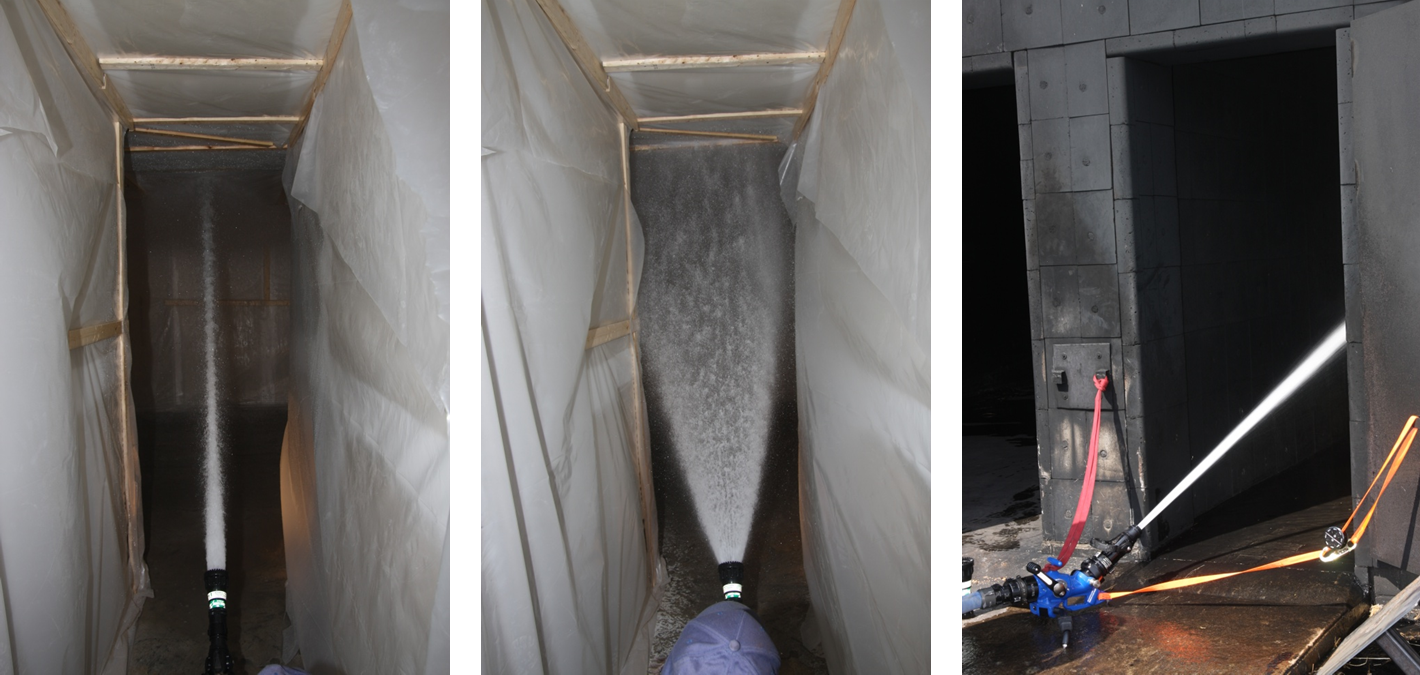
\includegraphics[width=6in]{../Figures/Pictures/Flows}
	\caption[Spray Density Nozzle Patterns]{Spray Density Nozzle Patterns. Left-To-Right: Straight Stream, Narrow Fog Stream, and Solid Stream.}
	\label{fig:Spray_Density_Nozzle_Patterns}
\end{figure}

\subsection{Gas Cooling}
\label{sec:desc_Gas_Cooling}

Eighty-eight experiments were conducted to study the effectiveness of cooling the upper gas layer in a space adjacent to the area of fire involvement. These tests examined five different hose stream patterns, two nozzle types, and both compressed air foam and water as the suppression agent. The focus of this experimental series was to study the impact of the test variables on the hot gas layer temperatures when a fixed hose stream was applied to a room adjacent to the fire room. Suppression agents were not applied to the fire in the burn room.  Detailed discussion of the tests and results are in Section~\ref{sec:Gas_Cooling}.

\subsection{Fire Suppression}
\label{sec:desc_Fire_Suppression}

The fire suppression series included 20 experiments. Twelve experiments were conducted in the single-story structures (6 in each structure) using both water and CAF application as a suppression agent. The nozzle patterns were varied and included straight stream, solid stream, and narrow fog stream. The six experiments in the two-story structure used both water and CAF from a straight stream nozzle.  In addition, two CAF experiments were conducted in the two-story burn building with a solid stream. 

\section{Experimental Facilities}
\label{sec:Experimental_Facility}

The series of tests described within this report were conducted at the Delaware County ESTC in Sharon Hill, PA. A burn building and two purpose-built concrete structures are located on the grounds of the ESTC. The burn building was used for the gas cooling experiments, and the purpose-built concrete structures were used for the fire suppression experiments. Figure~\ref{fig:Door_Status_Legend} provides the key for determining the status of open or closed doors in the facility schematics.

\begin{figure}[!ht]
	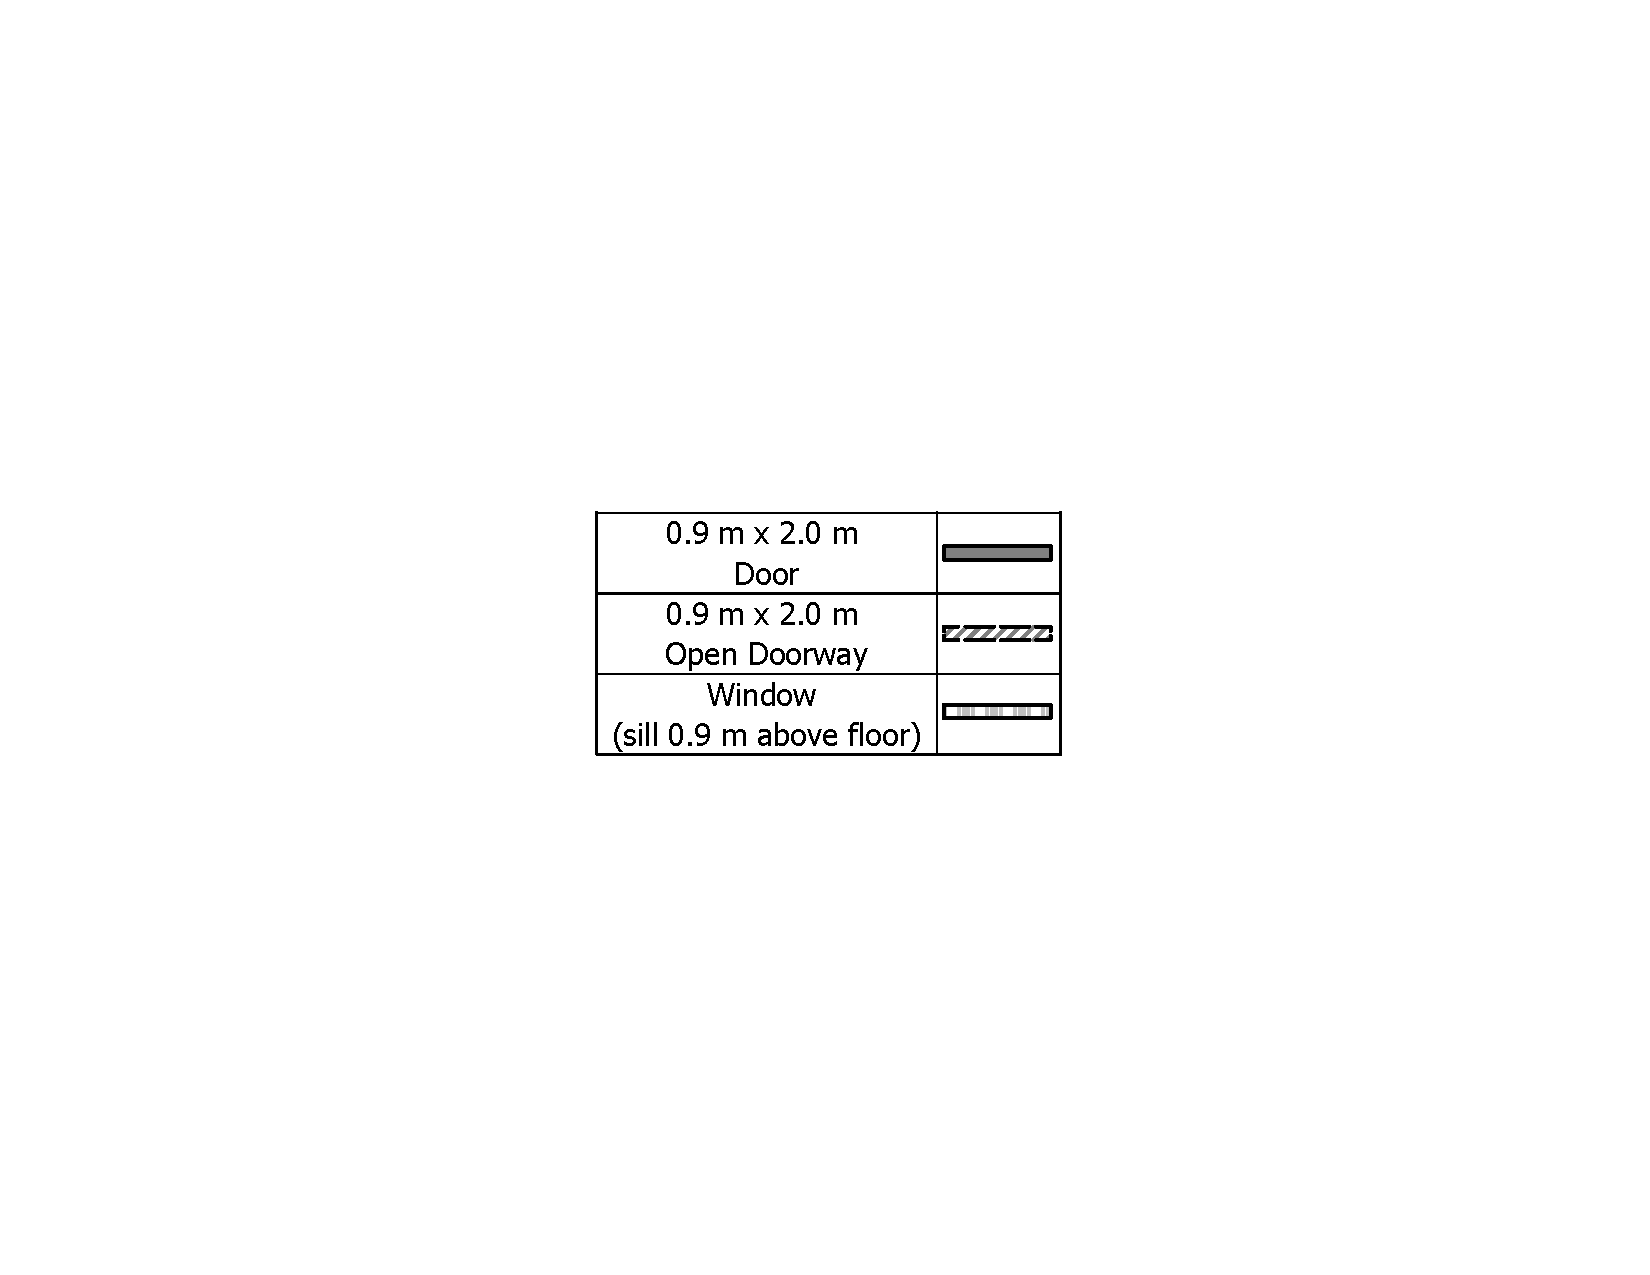
\includegraphics[width=.35\columnwidth]{../Figures/Floor_Plans/PDFs/DelCo_2012_Door_Legend}
	\caption{Door Status Legend}
	\label{fig:Door_Status_Legend}
\end{figure}

\subsection{Fire Training Structure}
\label{sec:Burn_Building}

The burn building, or live fire training structure, contained a two-story section and a three-story section. The building was supported with reinforced concrete beams and columns. The floors and ceilings were also concrete, and the interior walls were constructed of cement block. The walls and ceiling of the burn rooms were protected with a 25~mm (1~in) thick layer of calcium silicate insulation and was covered by 50~mm (2~in) thick concrete tile. The floors of the burn rooms were protected with fire brick. Tests were conducted on the ground floor of the two-story, two-room configuration, which had overall dimensions of 6.5~m (21.3~ft) by 9.2~m (30.2~ft). Figure~\ref{fig:Delaware_County,_PA_Burn_Building_Layout} contains a basic plan view of the test floor, and a fully dimensioned plan view of the floor is included in Appendix~\ref{app:floor_plans}.

\begin{figure}[!ht]
	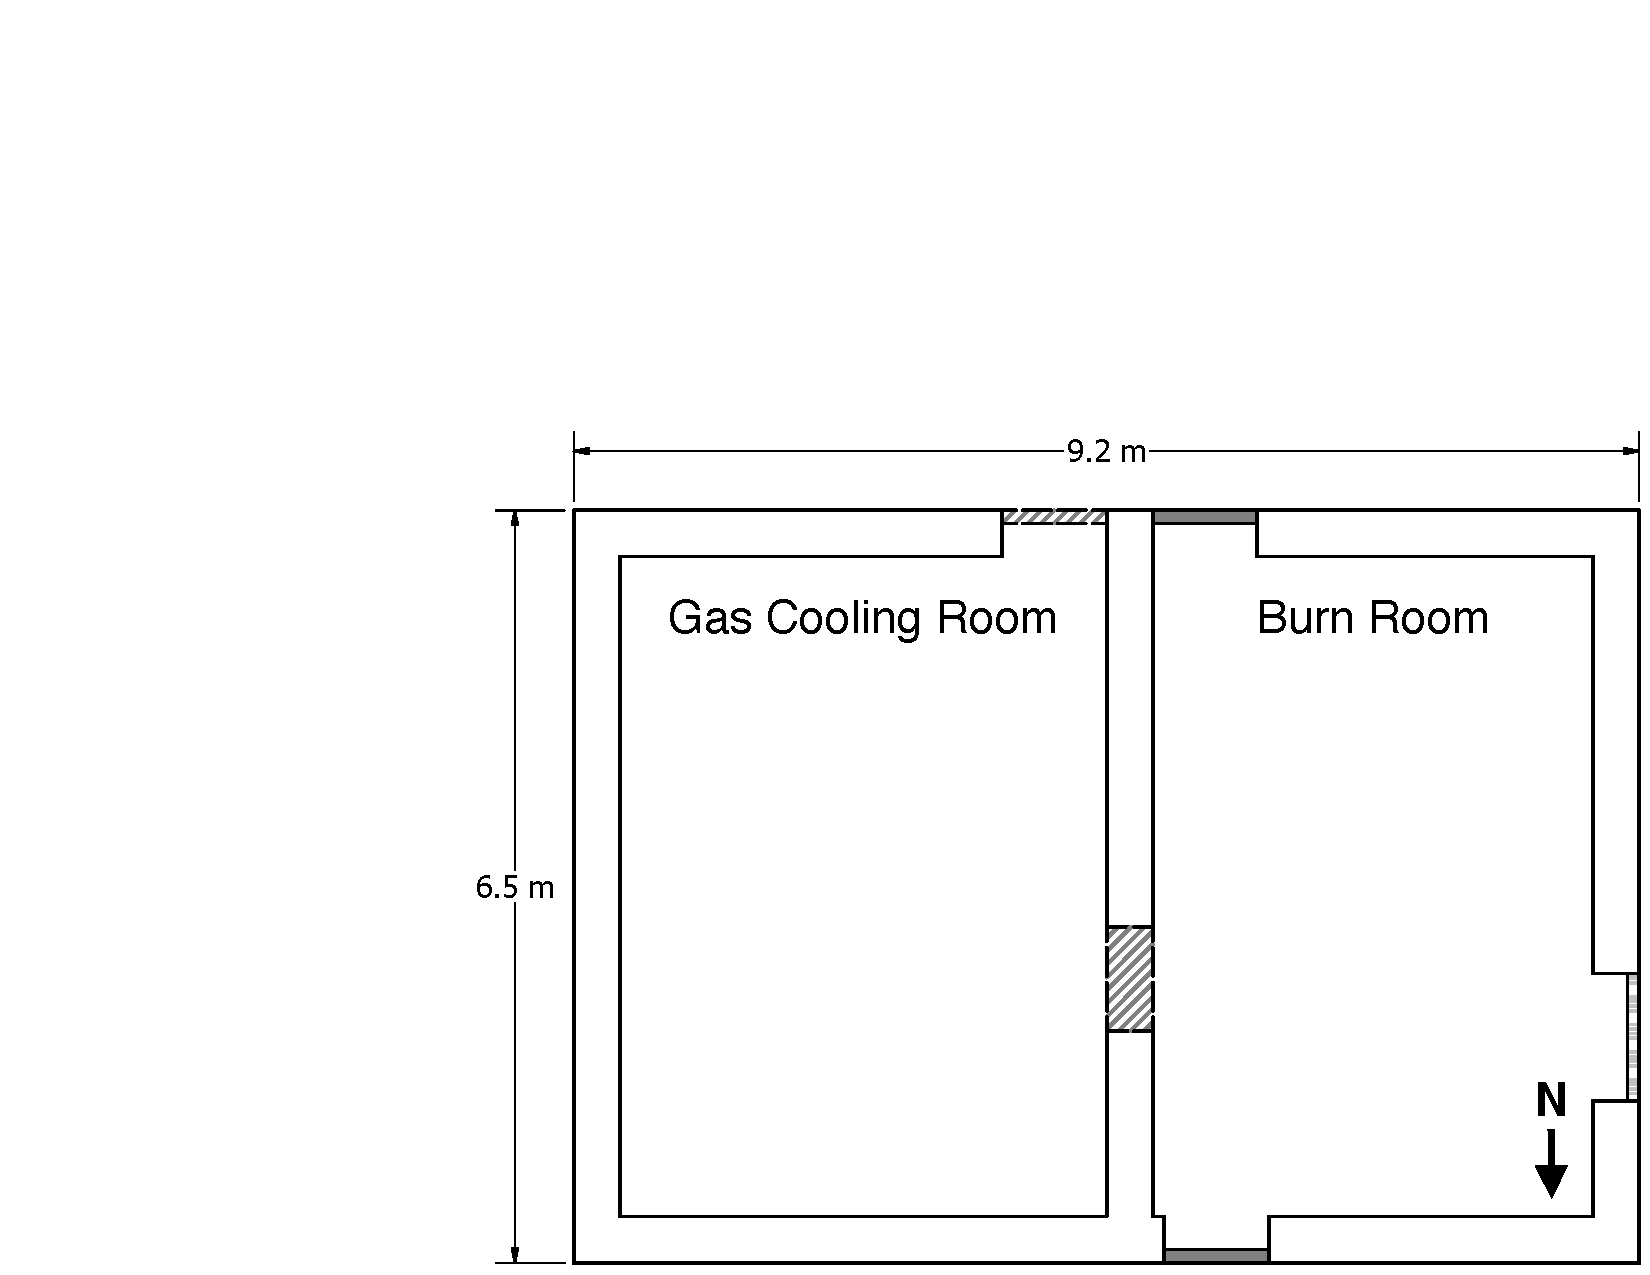
\includegraphics[width=\columnwidth]{../Figures/Floor_Plans/PDFs/West_Structure/DelCo_2012_West_Structure_Plain}
	\caption{Basic Floor Plan of the Burn Building Layout}
	\label{fig:Delaware_County,_PA_Burn_Building_Layout}
\end{figure}

The burn room where the fuel load was located measured 3.8~m (12.5~ft) by 5.7~m (18.7~ft) with a ceiling height of 3.35~m (11.0~ft). The adjacent room where the water was applied for gas cooling measured 4.1~m (13.4~ft) by 5.7~m (18.7~ft), also with a ceiling height of 3.35~m (11.0~ft). The open doorway that connected the burn room to the adjacent room and the doorway from the adjacent room to the exterior both measured 2.0~m (6.5~ft) high and 0.9~m (2.9~ft) wide.

\subsection{Concrete Block Structures}
\label{sec:Experimental Structures}
\subsubsection*{Single-Story Structures}

Two identical single-story concrete structures were built on a concrete slab as shown in Figure~\ref{fig:Delaware_County,_PA_Fire_Test_Structures}. They were designed to simulate a single floor of a residential structure.  The outer wall of each structure was composed of interlocking concrete blocks 0.61~m (2~ft) wide, 0.61~m (2~ft) high and 1.22~m (4~ft) long.  The interior dimensions of each structure were 6.1~m (20~ft) wide, 11~m (36~ft) long and 2.4~m (8~ft) high. The joints and gaps between the blocks were filled with high temperature insulation.

\begin{figure}[!ht]
	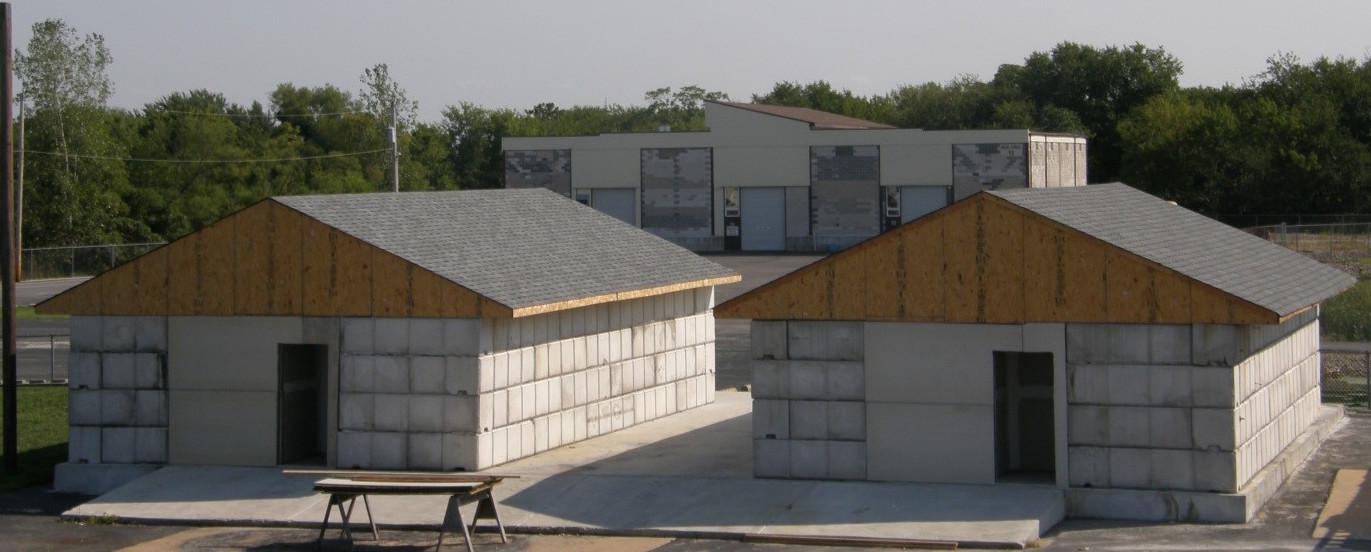
\includegraphics[width=6in]{../Figures/Pictures/DelCo_Structures}
	\caption{Delaware County, PA Fire Test Structures}
	\label{fig:Delaware_County,_PA_Fire_Test_Structures}
\end{figure}

Each structure had a burn room, approximately 6.0~m (19.6~ft) by 4.4~m (14.3~ft) and 2.74~m (9.0~ft) in height and a hallway connecting the burn room to the front of the structure via a small entry foyer. The hallway was 0.95~m (3.1~ft) wide and 5.4~m (17.6~ft) long and the entry foyer was 1.2~m (4.1~ft) by 1.9~m (6.1~ft). The ceiling height in the hallway and entry foyer was 2.4~m (8~ft).  The open door on north side from the exterior to the entry foyer was 2.0~m (6.5~ft) high and 0.9~m (2.9~ft) wide. The opening on the south face of the structure from the exterior to the burn room was 2.4~m (7.75~ft) high and 1.09~m (3.6~ft) wide. A basic plan view of the structure is presented in Figure~\ref{fig:Test_Structure_Floor_Plan}, and a fully dimensioned plan view of the structure is included in in Appendix~\ref{app:floor_plans}.

\begin{figure}[!ht]
	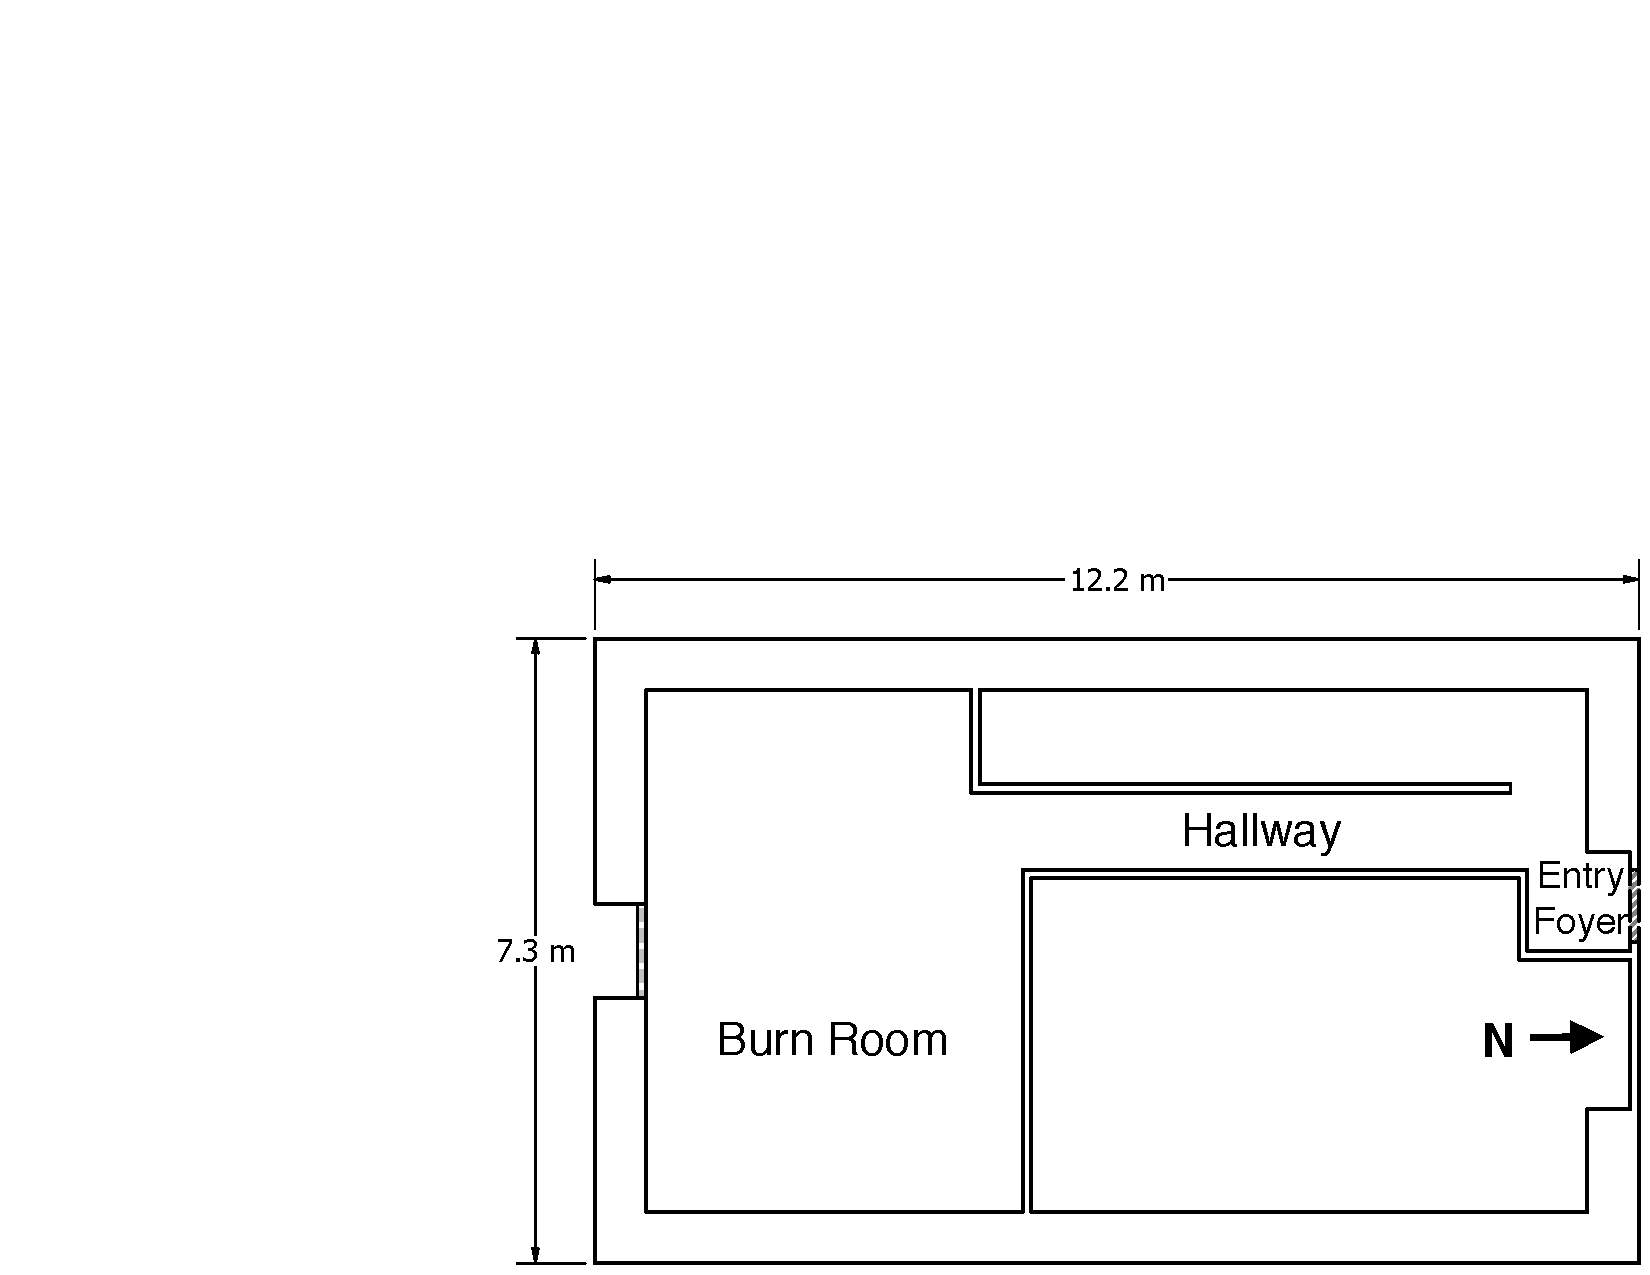
\includegraphics[width=\columnwidth]{../Figures/Floor_Plans/PDFs/East_Structure/DelCo_2012_East_Structure_Plain}
	\caption{Basic Floor Plan of the Single-Story Test Structure}
	\label{fig:Test_Structure_Floor_Plan}
\end{figure}

The floor of the structure was the concrete pad. The interior walls of the structure were framed with steel studs and track. The studs were set to 0.40~m (16~in) centers. The ceiling support was composed of wood truss joist I-beams (TJIs) with a 299~mm (11.75~in) depth. The TJI was composed of laminated veneer lumber flanges with a cross section of 29~mm (1.13~in) x 44~mm (1.75~in) and an 11~mm (0.43~in) thick oriented strand board web. Tongue and grove, 18.3~mm (0.72~in) thick, oriented strand board was attached to the top of the TJIs.

The interior walls of the burn room were lined with 13~mm (0.5~in) thick cement board. The ceiling of the burn room was the exposed ``floor assembly''. The walls of the hallway and entry foyer were composed of 16~mm (0.63~in) Type X gypsum board. The ceiling of the hallway and entry foyer was composed of two layers of 13~mm (0.5~in) thick cement board.

\subsubsection*{Two-Story Structure}

A second story was added to the west single-story structure in order to test larger fires and remote suppression effects (see Figure~\ref{fig:delco_2story}).

\begin{figure}[!ht]
	\includegraphics[width=6in]{../Figures/Pictures/DelCo}
	\caption{Delaware County, PA Two-Story Fire Test Structure}
	\label{fig:delco_2story}
\end{figure}

The outer walls of the bottom floor of the two-story structure were identical to that of the single-story structures described above but with an open floor plan. The interior dimensions were 6.1~m (20~ft) wide, 11~m (36~ft) long and 2.4~m (8~ft) high. Figure~\ref{fig:dimensioned_first_2story} shows a basic floor plan of the reconfigured first floor. A fully dimensioned plan view of the floor is included in Appendix~\ref{app:floor_plans}. A stairwell was built to connect the two floors of the structure. The stairs had a 180~mm (7.25~in) rise and 190~mm (7.5~in) run and started 1.6~m (5.25~ft) off the south wall with a width of 1.2~m (4~ft) off the east wall. The second story walls were wood framed with 51~mm (2~in) by 102~mm (4~in) studs. The studs were set to 0.40~m (16~in) centers. The interior  walls were protected by 16~mm (0.63~in) fire rated gypsum board, 16~mm (0.63~in) Durock board, and a second layer of 16~mm (0.63~in) fire rated gypsum board. The exterior walls were protected with 11~mm (0.31~in) oriented strand board and 8~mm (0.31~in) fiber cement lap siding. Figure~\ref{fig:dimensioned_second_2story} shows a basic floor plan of the second story of the modified west structure, and a fully dimensioned plan view of the floor is included in Appendix~\ref{app:floor_plans}.

\begin{figure}[!ht]
	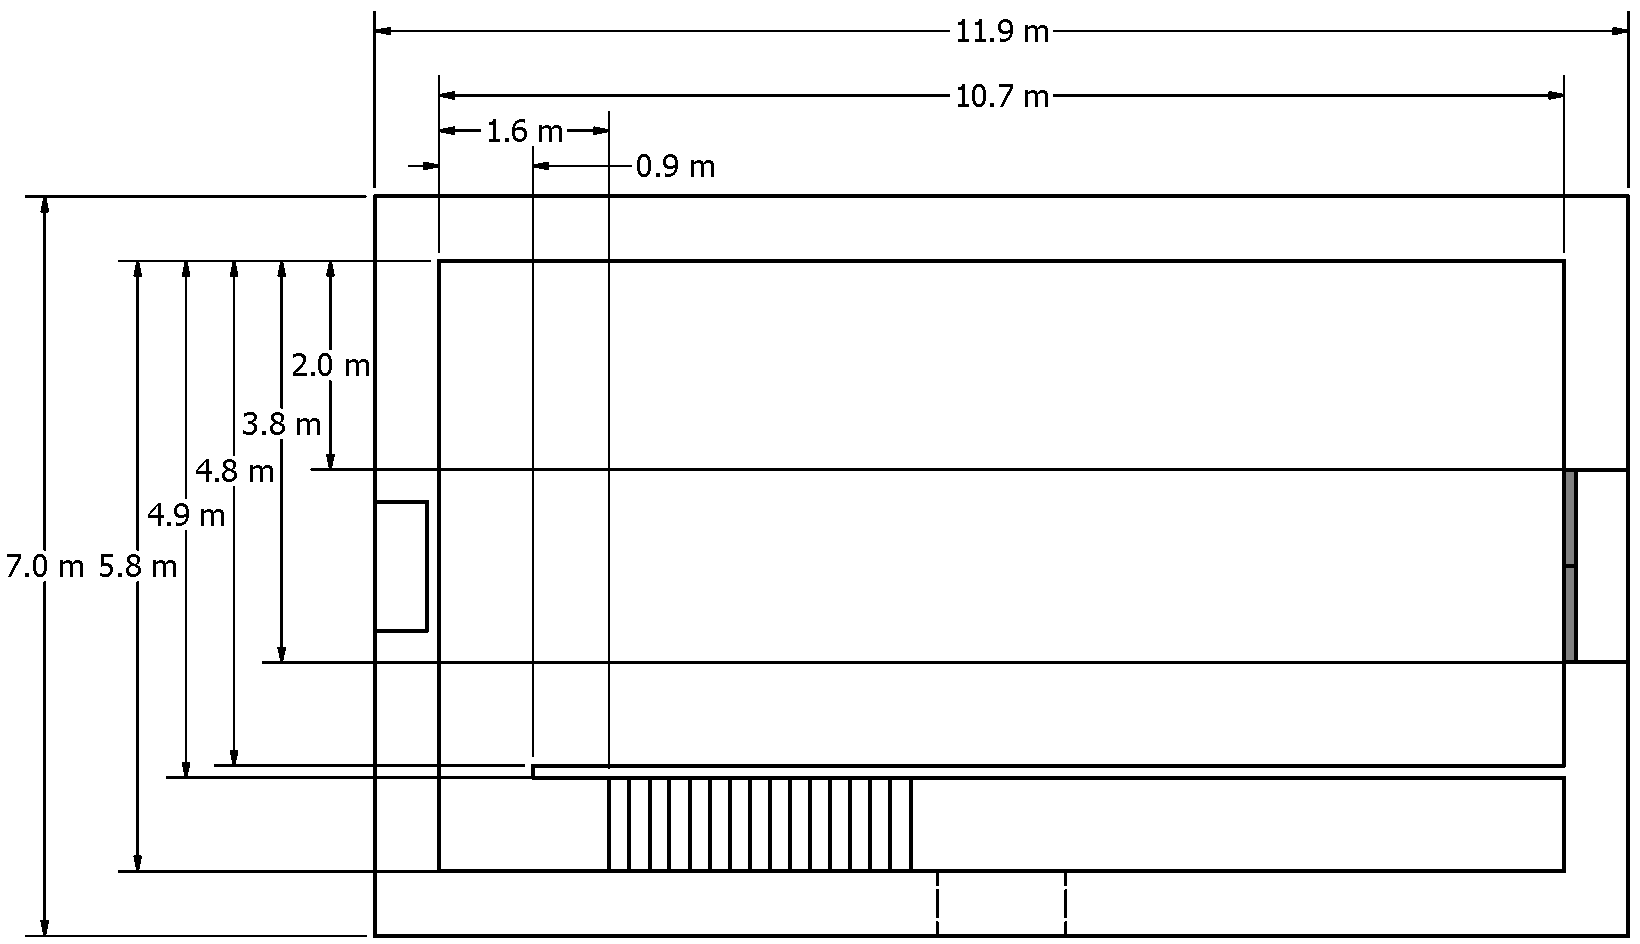
\includegraphics[width=\columnwidth]{../../DelCo_2014_2015/Drawings/PDFs/CAFS/West_Structure_1st_Floor_Plain}
	\caption{Basic Floor Plan of the First Floor of the Two-Story Structure}
	\label{fig:dimensioned_first_2story}
\end{figure}


\begin{figure}[!ht]
	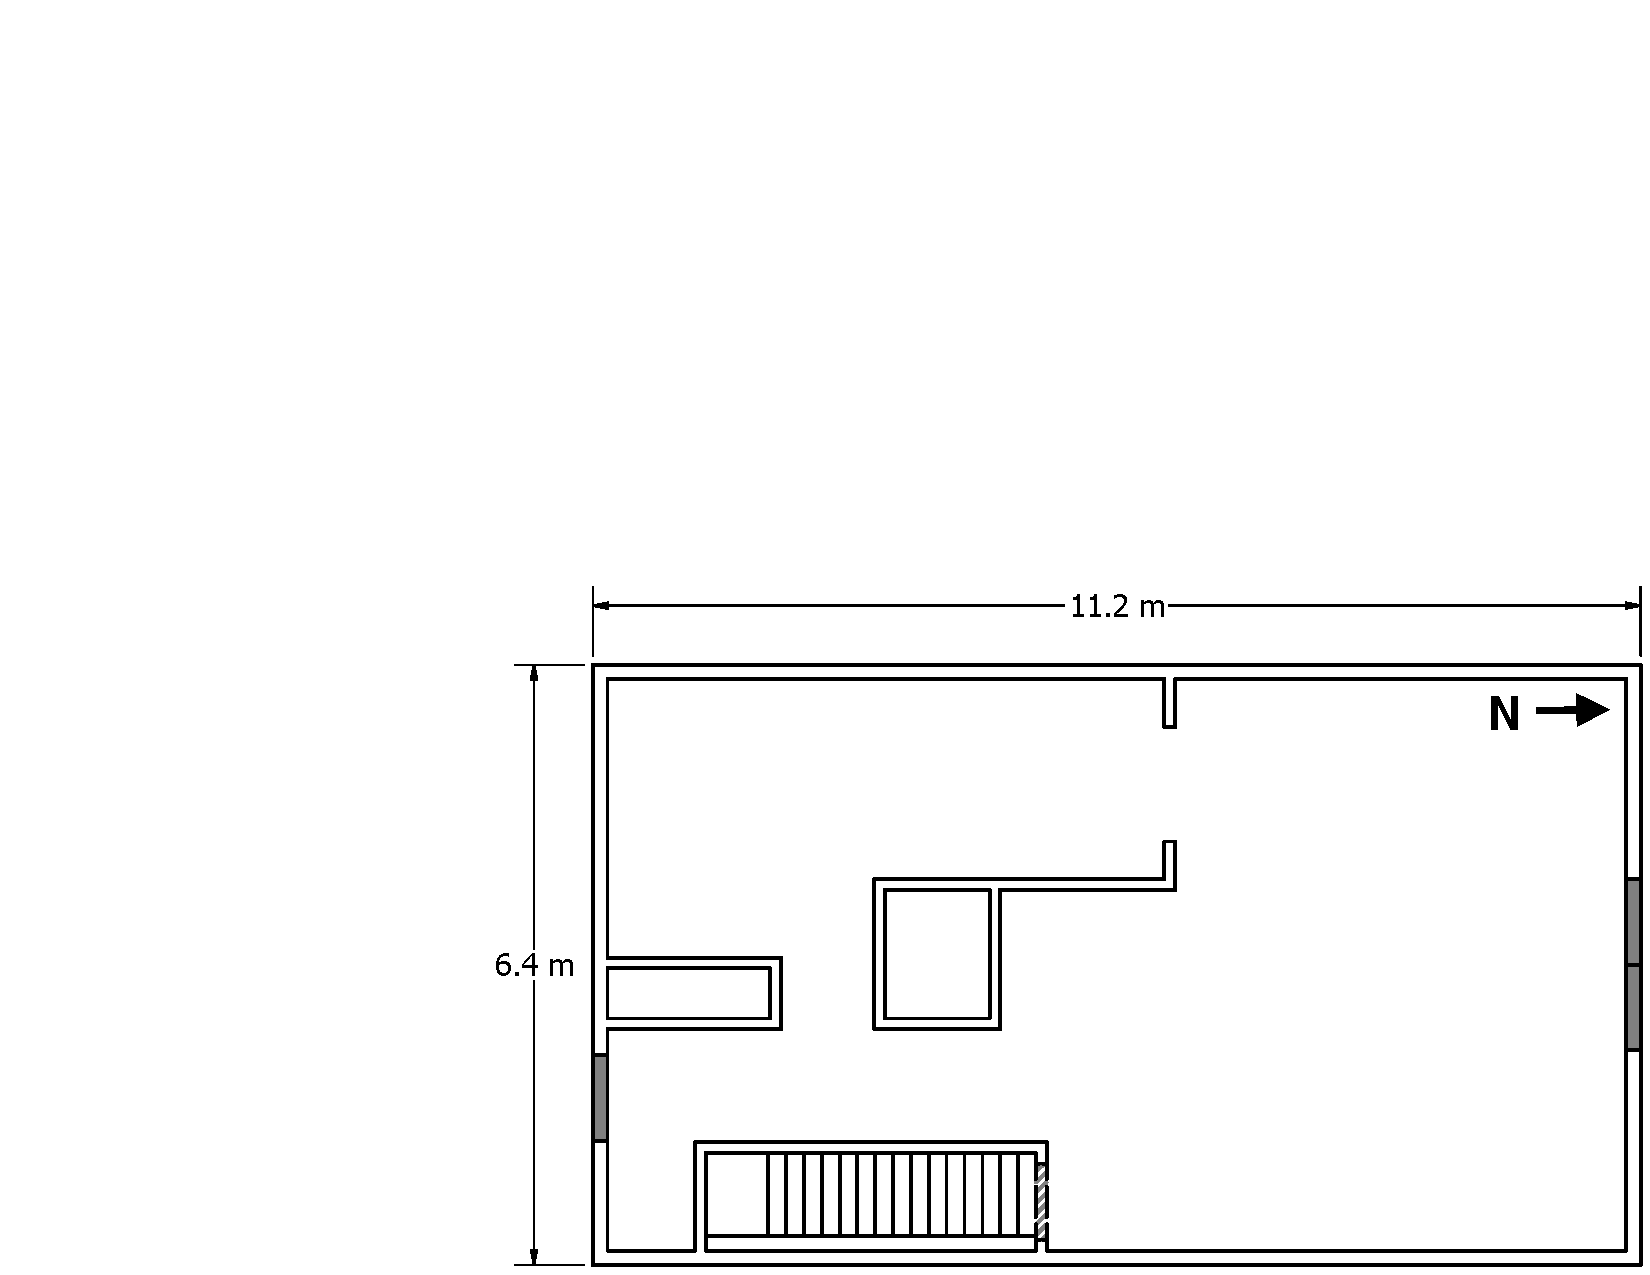
\includegraphics[width=\columnwidth]{../../DelCo_2014_2015/Drawings/PDFs/CAFS/West_Structure_2nd_Floor_Plain}
	\caption{Basic Floor Plan of the Second Floor of the Two-Story Structure}
	\label{fig:dimensioned_second_2story}
\end{figure}

\clearpage

\section{Instrumentation}
\label{sec:Instrumentation}

The structures were instrumented for gas temperature, gas velocity, and heat flux measurements. Gas temperatures in the burn rooms were measured with bare-bead, Chromel-Alumel (type K) thermocouples. Additional single, sheathed thermocouples were installed in conjunction with the bi-directional probes for gas velocity measurements. The single thermocouples were bare-bead, Chromel-Alumel (type K) thermocouples with a 1.0~mm (0.04~in) nominal diameter. The thermocouple was protected with an 3.2~mm (0.13~in) diameter inconel sheath. The sheathing protects the thermocouple from water but slows the response time because of the additional thermal mass. Schmidt-Boelter gauges were used to measure both total heat flux and radiant heat flux (radiometer). A radiometer is a total heat flux gauge with a zirconium plate to prevent contributions from convective heat transfer. A legend, which clarifies the instrumentation schematics discussed in the following sections, is included in Figure~\ref{fig:Instrumentation_Legend}.

\begin{figure}[!ht]
	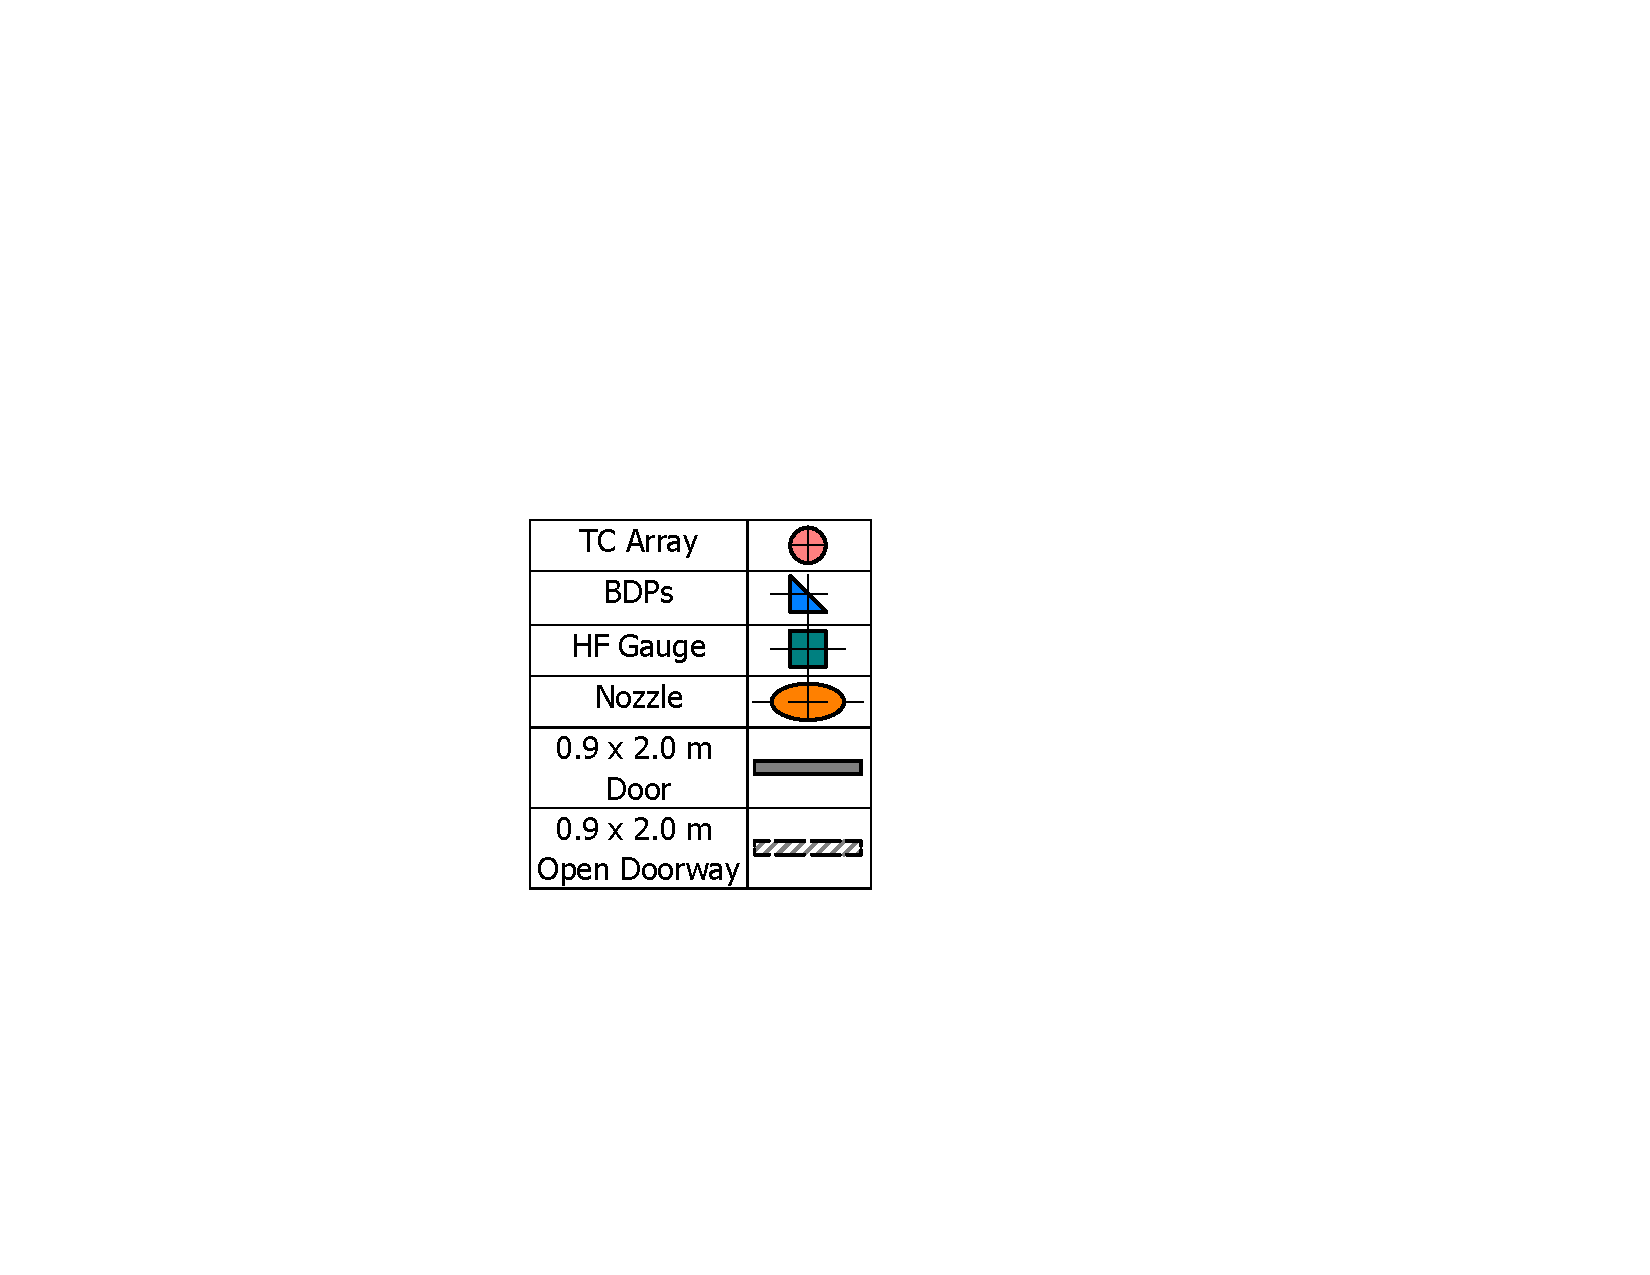
\includegraphics[width=.35\columnwidth]{../Figures/Floor_Plans/PDFs/DelCo_2012_Instrumentation_Legend}
	\caption{Instrumentation Legend}
	\label{fig:Instrumentation_Legend}
\end{figure}

\subsection{Gas Cooling}
\label{subsec:Gas_Cooling_Instrumentation}

The gas cooling tests included four bare-bead thermocouple arrays, a bi-directional probe with a thermocouple array, and a total heat flux gauge/radiometer pair. Figure~\ref{fig:Gas_Cooling_Instrumentation_Dimensions} provides the positions within the burn room and gas cooling room where the sensors were located (see Figure~\ref{fig:Instrumentation_Legend} for reference on the symbols). Each of the bare-bead thermocouple arrays had 11 thermocouples. The top thermocouple was placed at the ceiling and each subsequent thermocouple was spaced 0.3~m (1~ft) apart with the bottom thermocouple being 3.05~m (10~ft) below the ceiling. There were six velocity probes and solid thermocouples centered at the external doorway to the gas cooling room. The top probe was 0.15~m (0.5~ft) below the door soffit, the second probe was 0.3~m (1~ft) below the soffit, and the remaining four were spaced 0.3~m (1~ft) apart with the bottom probe being 1.52~m (5~ft) below the soffit. The total heat flux gauge/radiometer set was positioned 0.15~m (0.5~ft) off the ground and aimed to view the ceiling.

\begin{figure}[!ht]
	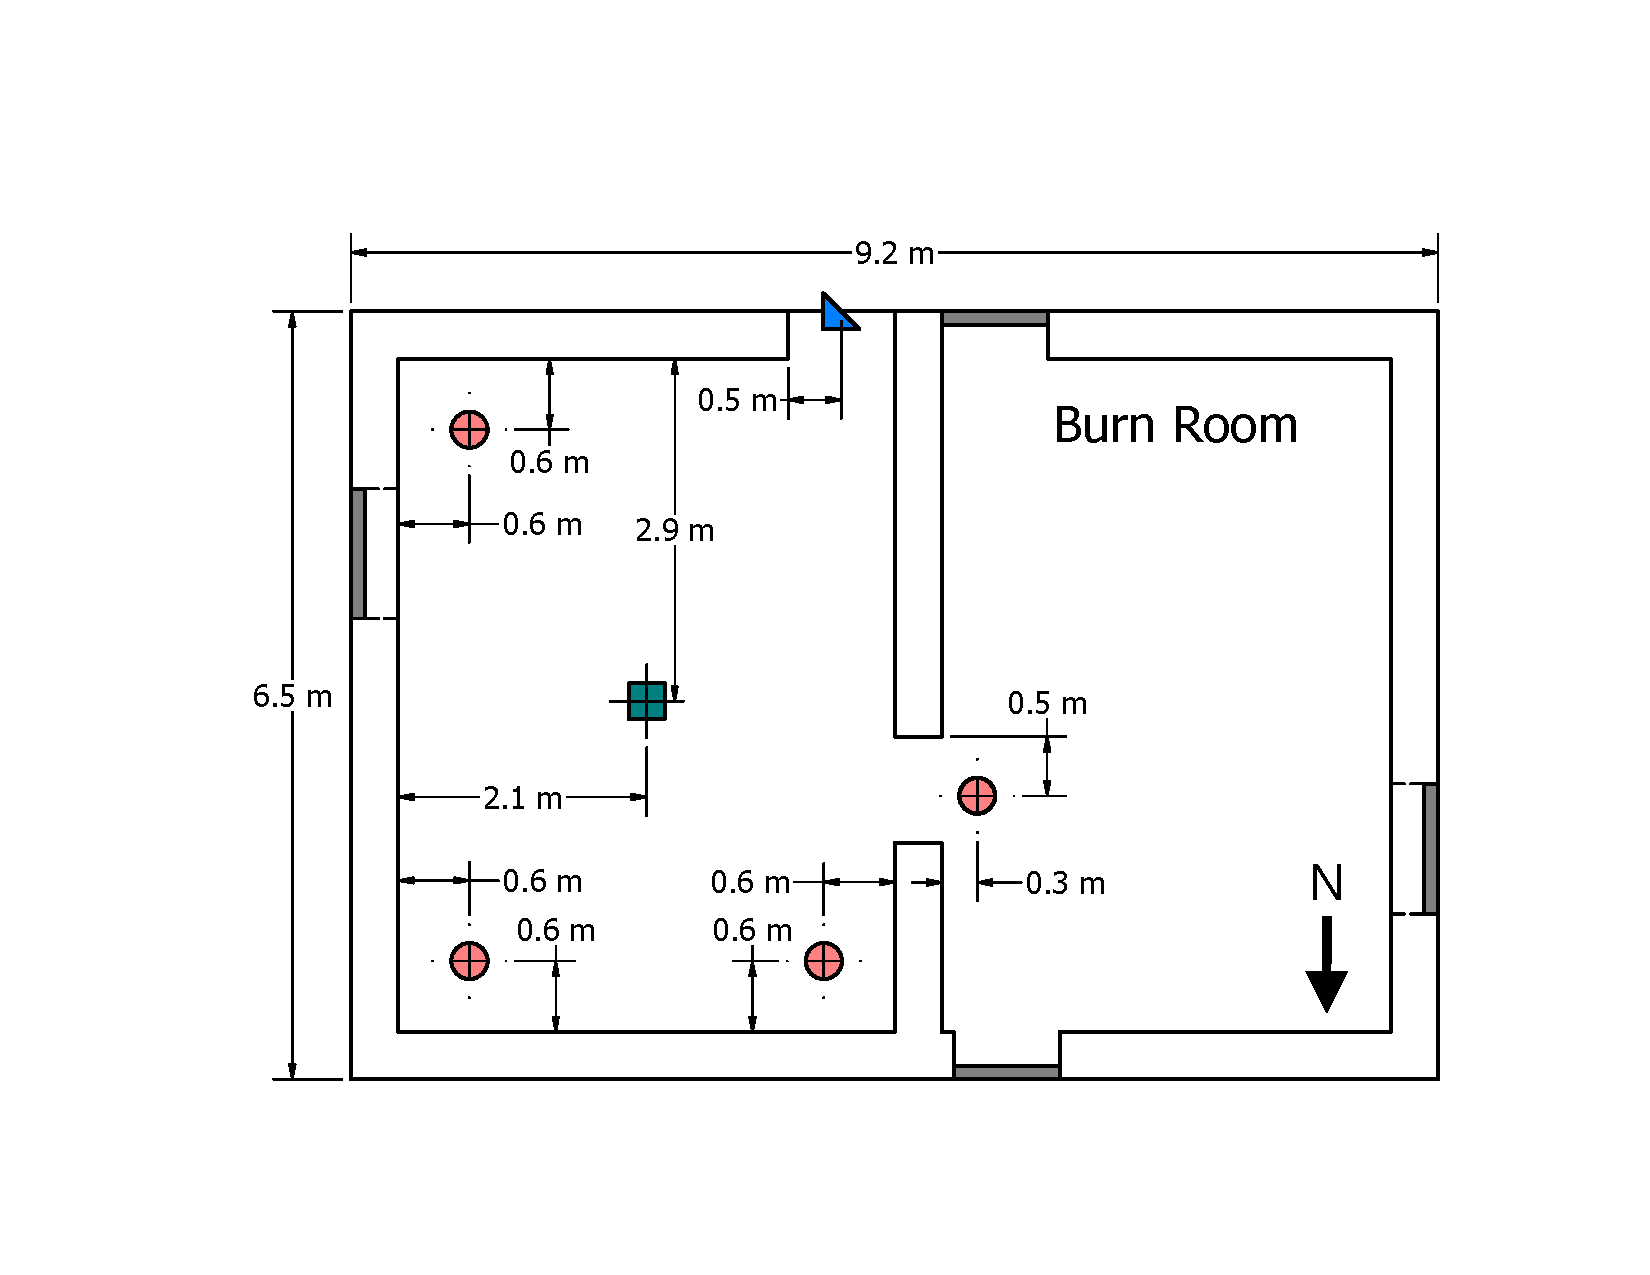
\includegraphics[width=\columnwidth]{../Figures/Floor_Plans/PDFs/West_Structure/DelCo_2012_West_Structure_Instrumentation}
	\caption{Instrumentation Schematic for the Gas Cooling Experiments}
	\label{fig:Gas_Cooling_Instrumentation_Dimensions}
\end{figure}

\clearpage

\subsection{Fire Suppression}
\label{subsec:Fire_Suppression_Instrumentation}

\subsubsection*{Single-Story Structure}

The fire suppression testing in the single-story structure included two bare-bead thermocouple arrays, three bi-directional probe plus solid thermocouple arrays, two total heat flux gauge pairs, and two total heat flux gauge/radiometer pairs. Figure~\ref{fig:Fire_Suppression_Instrumentation_Dimensions} provides the positions within the burn room, hallway, and entrance foyer where the sensors were located (see Figure~\ref{fig:Instrumentation_Legend} for reference on the symbols). Each bare-bead thermocouple array had eight thermocouples. The top sensor was 0.03~m (1~in) below the ceiling and the remaining thermocouples were spaced 0.3~m (1~ft) apart with the bottom thermocouple being 2.13~m (7~ft) below the ceiling. The three bi-directional probe arrays had unique sensor locations. For the window array, there were four sensor pairs located 0.28~m (0.95~ft), 0.58~m (1.90~ft), 0.84~m (2.85~ft), and 1.16~m (3.8~ft) below the soffit. For the hallway array, the seven sensor pairs started 0.3~m (1~ft) below the ceiling and were spaced every 0.3~m (1~ft) ending 2.13~m (7~ft) below the ceiling. The doorway array also had seven sensor pairs, but the first pair was located 0.15~m (0.5~ft) below the soffit. The remaining sensors were spaced every 0.3~m (1~ft) with the bottom pair 1.83~m (6~ft) below the doorway soffit. The total heat flux gauge/radiometer pairs were set to be 0.15~m (0.5~ft) off the ground and aimed to view the ceiling. The pairs of total heat flux gauges were set 1~m (3~ft) off the ground with one sensor ``looking'' vertical at the ceiling and the other horizontal.

\begin{figure}[!ht]
	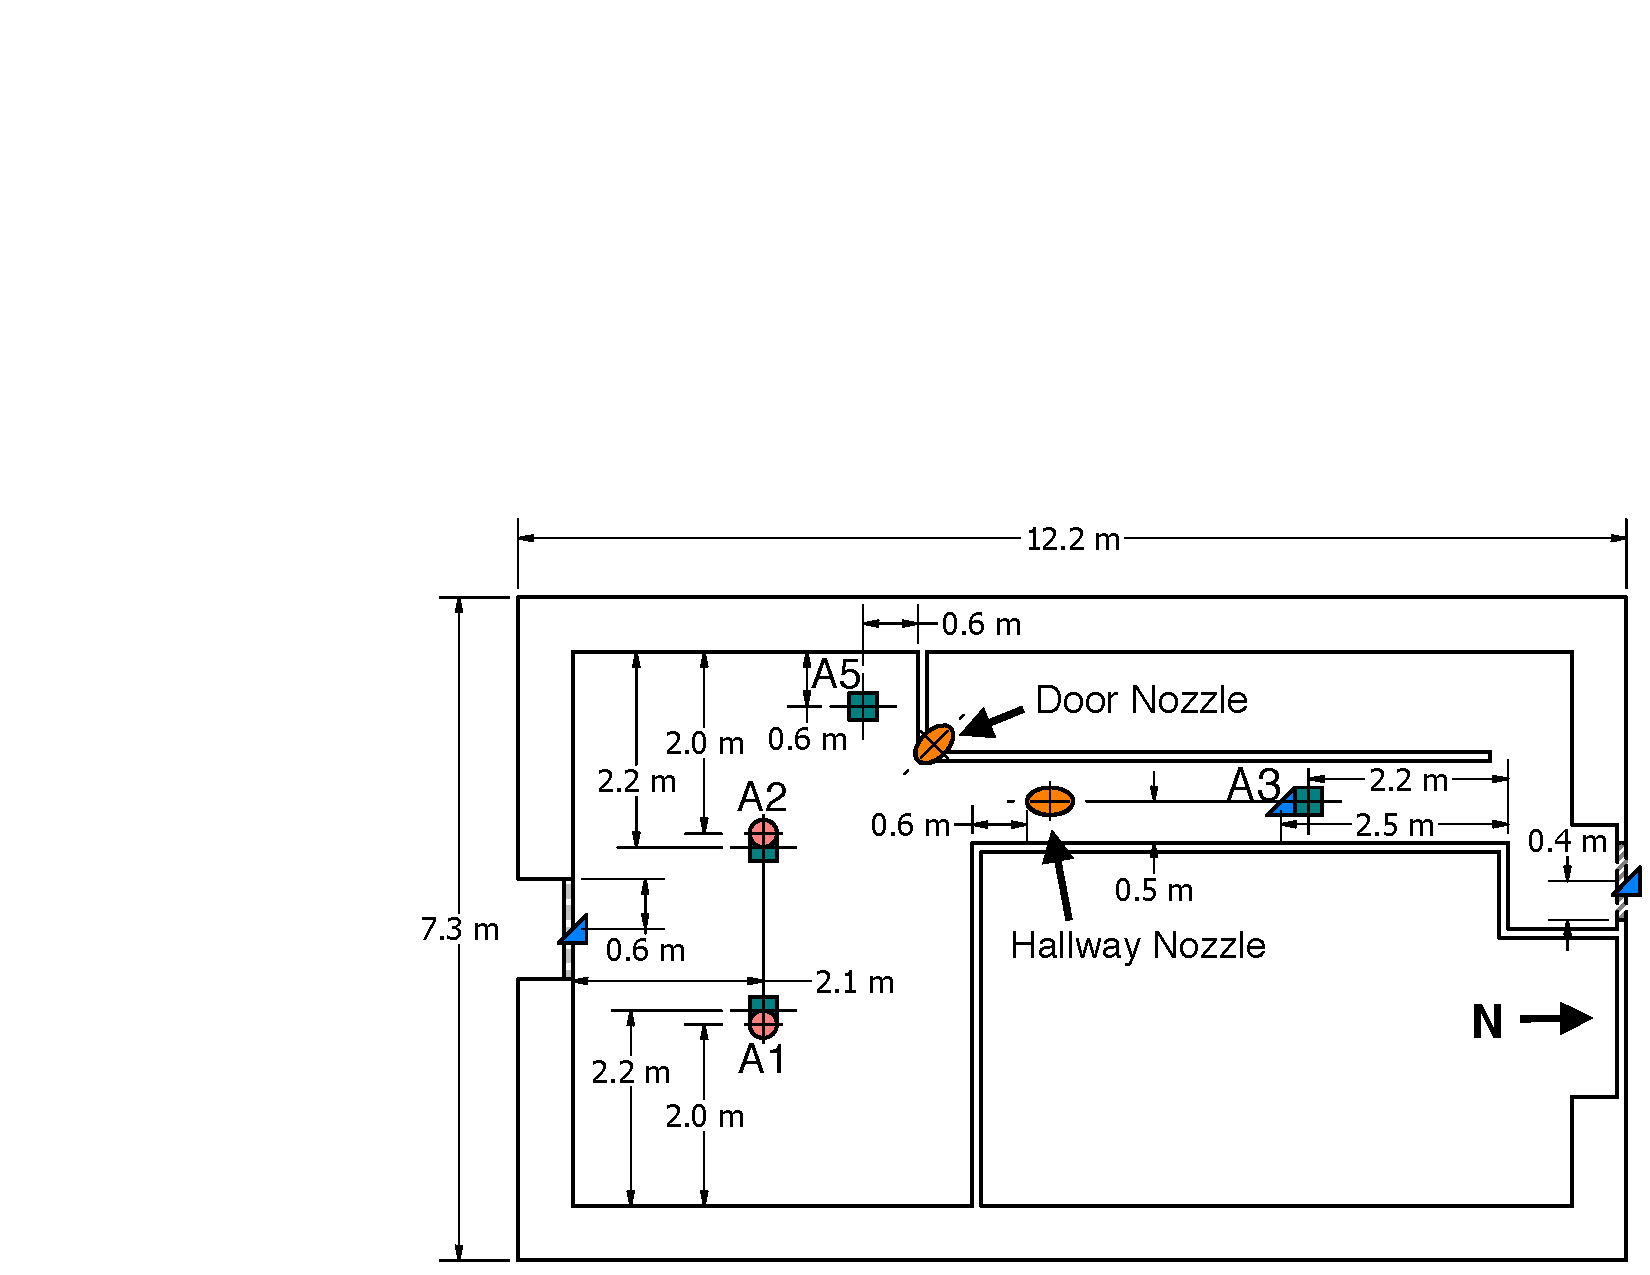
\includegraphics[width=\columnwidth]{../Figures/Floor_Plans/PDFs/East_Structure/DelCo_2012_East_Structure_Instrumentation}
	\caption{Instrumentation Schematic for the Single-Story Fire Suppression Experiments}
	\label{fig:Fire_Suppression_Instrumentation_Dimensions}
\end{figure}

\subsubsection*{Two-Story Structure}

Fire suppression testing in the two-story structure included similar types of instrumentation but with more sensors. Three bare-bead thermocouple arrays and two bi-directional probe and thermocouple arrays were used in the first floor. Figure~\ref{fig:fire_supp_first_2story} shows the positions of the instrumentation (see Figure~\ref{fig:Instrumentation_Legend} for reference on the symbols). Each of the bare-bead arrays had eight thermocouples with the same spacing as the single-story tests. The bi-directional probe and solid thermocouple arrays also had eight sensors with the first probe 0.08~m (0.25~ft) below the soffit and the remaining probes at 0.34~m (1.1~ft), 0.61~m (2~ft), 0.88~m (2.9~ft), 1.15~m (3.7~ft), 1.42~m (4.7~ft), 1.68~m (5.5~ft), and 1.95~m (6.4~ft) below the soffit.

\begin{figure}[!ht]
	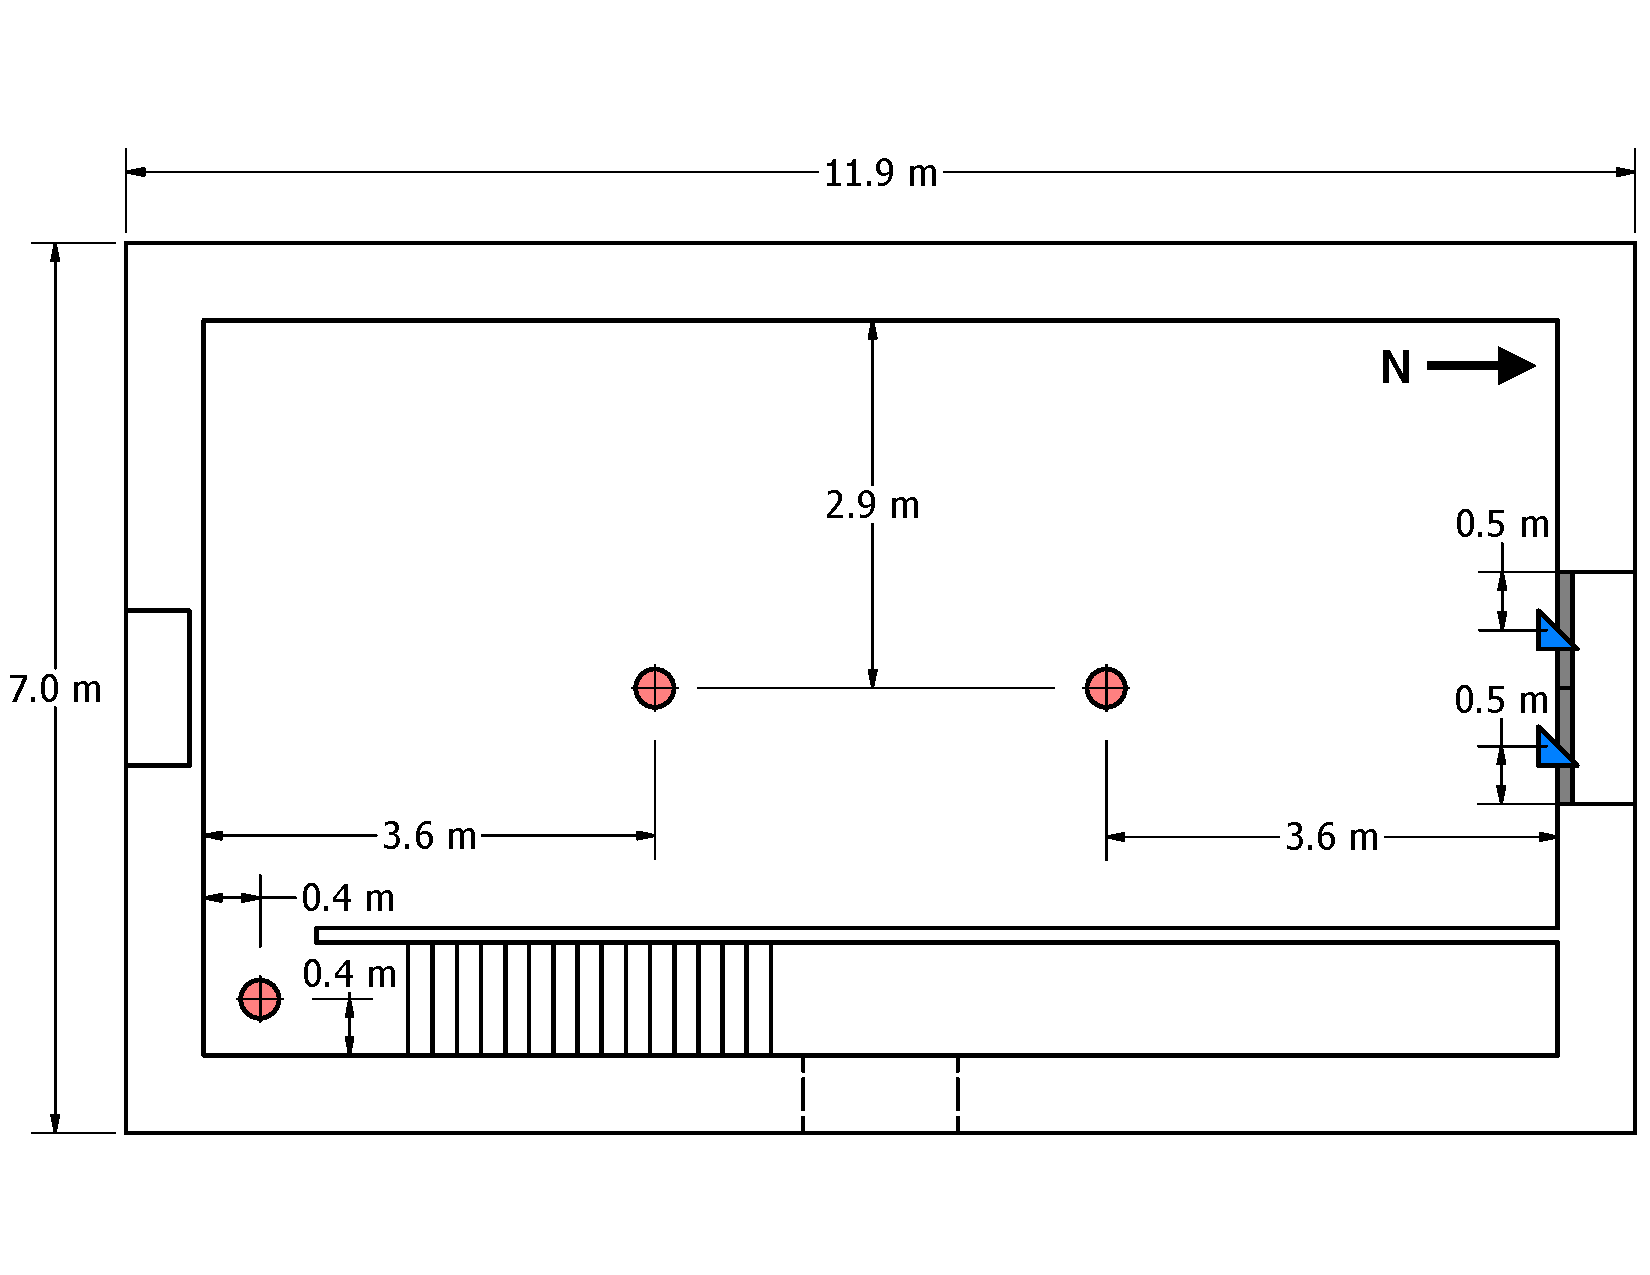
\includegraphics[width=\columnwidth]{../../DelCo_2014_2015/Drawings/PDFs/CAFS/West_Structure_1st_Floor_Instrumentation}
	\caption{Instrumentation Schematic for the First Floor of Fire Suppression Experiments in Two-Story Structure}
	\label{fig:fire_supp_first_2story}
\end{figure}

The second story featured six bare-bead arrays and three bi-directional probe plus solid thermocouple arrays. The second floor also had three heat flux sensor pairs (one facing horizontal and one facing vertical) that were 1~m (3~ft) off the ground. Figure~\ref{fig:fire_supp_second_2story} shows the positions of the instrumentation (see Figure~\ref{fig:Instrumentation_Legend} for reference on the symbols). The bare-bead thermocouple arrays featured eight sensors with the same spacing as the basement level. The bi-directional probe arrays at the south wall door and at the top of the stairwell were comprised of eight sensor pairs with the same spacing as the ground level. The third bi-directional probe array (3~m (9~ft) off the north wall and 0.6~m (2~ft) off the east wall) had eight sensor pairs with the same spacing at the bare-bead thermocouple arrays.

\begin{figure}[!ht]
	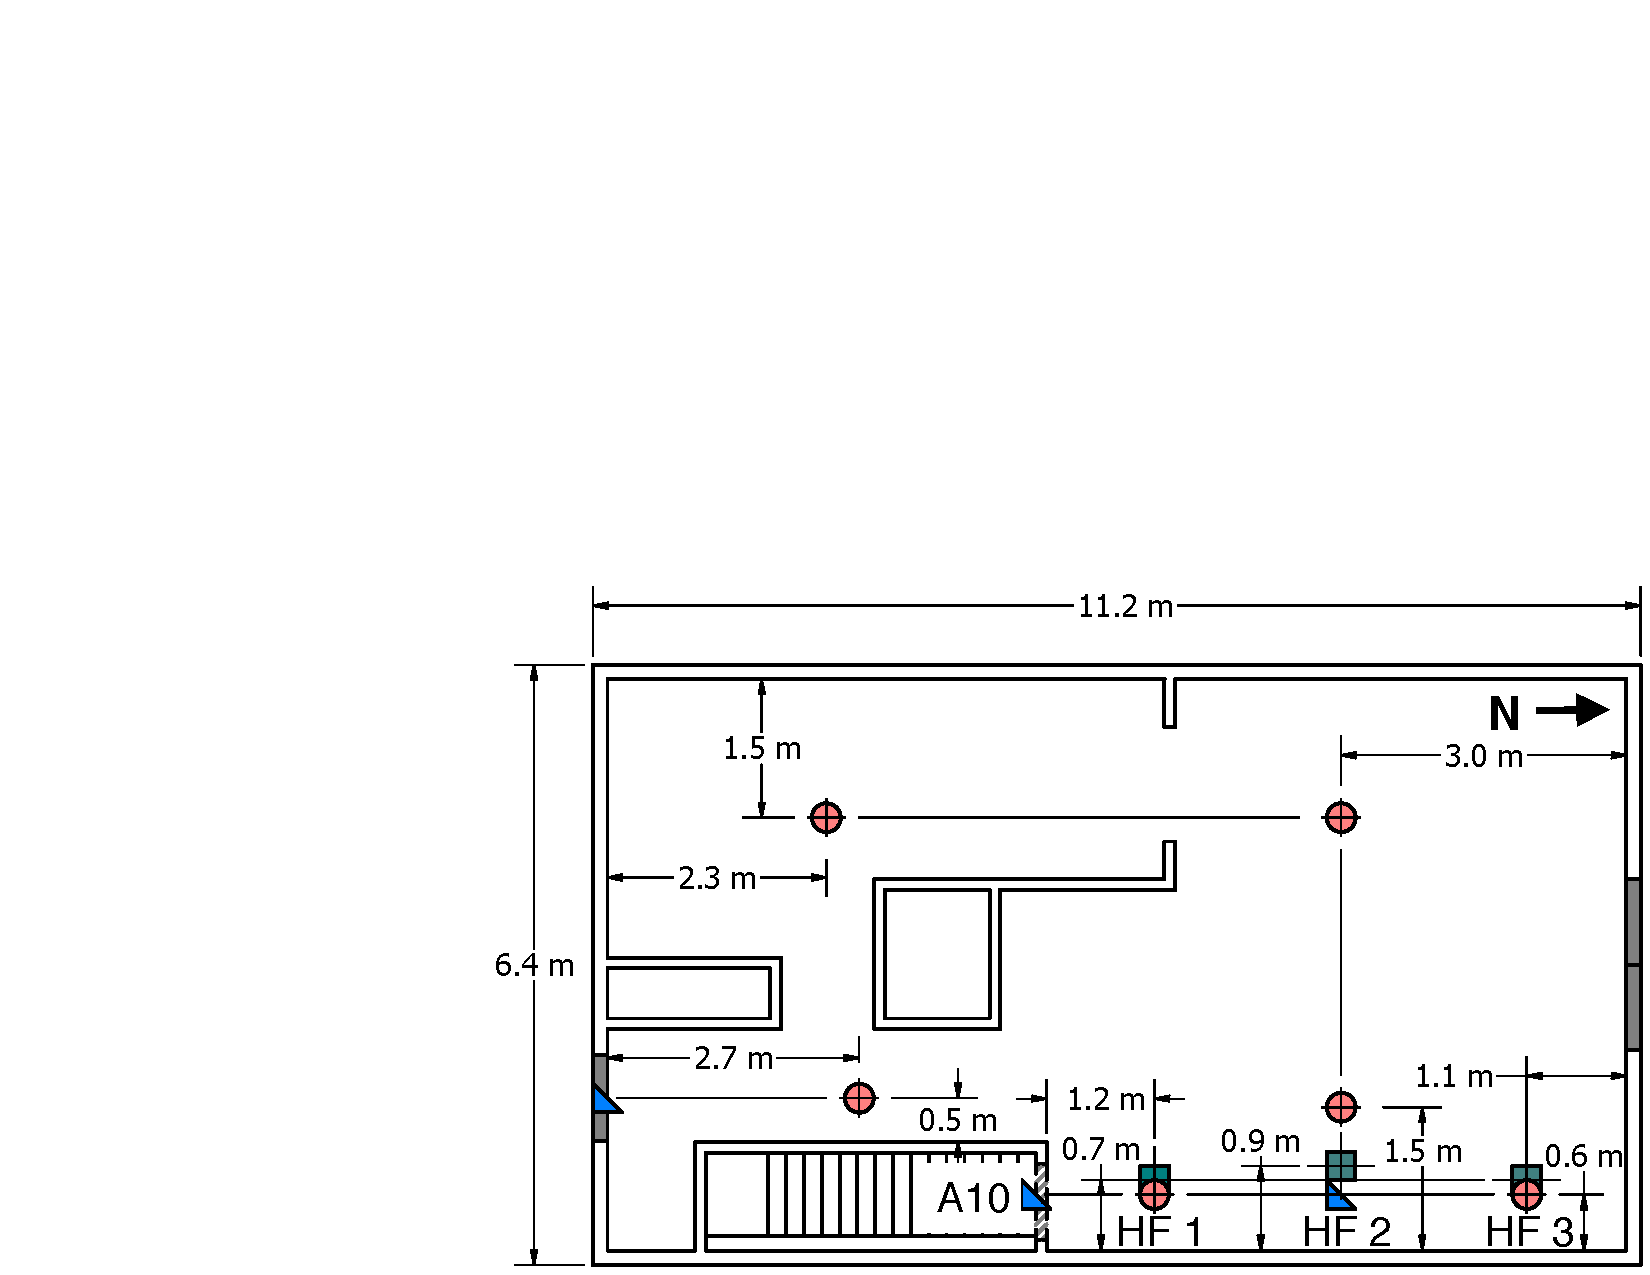
\includegraphics[width=\columnwidth]{../../DelCo_2014_2015/Drawings/PDFs/CAFS/West_Structure_2nd_Floor_Instrumentation}
	\caption{Instrumentation Schematic for the Second Floor of Fire Suppression Experiments in Two-Story Structure}
	\label{fig:fire_supp_second_2story}
\end{figure}

\clearpage

\subsection{Measurement Uncertainty}
\label{subsec:Uncertainty}

There are different components of uncertainty in the length, mass, temperature, heat flux, gas concentration, differential pressure, gas velocity, and heat release rate reported here. Uncertainties are grouped into two categories according to the method used to estimate them. Type A uncertainties are those which are evaluated by statistical methods, and Type B are those which are evaluated by other means~\cite{Taylor&Kuyatt:1994}. Type B analysis of systematic uncertainties involves estimating the upper (+~a) and lower (-~a) limits for the quantity in question such that the probability that the value would be in the interval ($\pm$~a) is essentially 100~\%. After estimating uncertainties by either Type A or B analysis, the uncertainties are combined in quadrature to yield the combined standard uncertainty. Then, the combined standard uncertainty is multiplied by a coverage factor of two, which results in the expanded uncertainty with a 95~\% confidence interval (2$\sigma$).  For some of these components, such as the zero and calibration elements, uncertainties are derived from referenced instrument specifications. For other components, referenced research results and past experience with the instruments provided input in the uncertainty determination.

Each length measurement was taken carefully. Length measurements, such as the room dimensions, instrumentation array locations, and fire apparatus (e.g., nozzle, sprinkler, or fan) placement, were made with a hand held laser measurement device that had an accuracy of $\pm$~6.0~mm (0.25~in) over a range of 0.61~m (2.0~ft) to 15.3~m (50.0~ft)~\cite{StanleyTools}. However, conditions affecting the measurement, such as levelness of the device, yields an estimated uncertainty of $\pm$~0.5~\% for measurements in the 2.0~m (6.6~ft) to 10.0~m (32.8~ft) range.  Steel measuring tapes with a resolution of  $\pm$~0.5~mm (0.02~in) were used to locate individual sensors within an instrumentation array and to measure and position the furniture. The steel measuring tapes were manufactured in compliance with NIST Manual 44, which specifies a tolerance of $\pm$~1.6~mm (0.06~in) for 9.1~m (30~ft) tapes and $\pm$~6.4~mm (0.25~in) for 30.5~m (100~ft) tapes~\cite{Butcher:2012}. Some issues, such as ``soft'' edges on the upholstered furniture, result in an estimated total expanded uncertainty of $\pm$~1.0~\%.

The load cell used to weigh the fuels prior to the experiments had a range of 0~kg (0~lb) to 200~kg (440~lb) with a resolution of a 0.05~kg (0.11~lb) and a calibration uncertainty within 1~\%~\cite{Ohaus:2000}. The expanded uncertainty is estimated to be less than $\pm$~5~\%.

The standard uncertainty in temperature of the thermocouple wire itself is $\pm$~2.2~$^{\circ}$C at 277~$^{\circ}$C and increases to $\pm$~9.5~$^{\circ}$C at 871~$^{\circ}$C as determined by the wire manufacturer~\cite{Omega:2004}. The variation of the temperature in the environment surrounding the thermocouple is known to be much greater than that of the wire uncertainty~\cite{Blevins:1999,Pitts:2003}. Small diameter thermocouples were used to limit the impact of radiative heating and cooling. The estimated total expanded uncertainty for temperature in these experiments is $\pm$~15~\%.

In this study, total heat flux measurements were made with water-cooled Schmidt-Boelter gauges. The manufacturer reports a $\pm$~3~\% calibration expanded uncertainty for these devices~\cite{Medtherm:2003}. Results from an international study on total heat flux gauge calibration and response demonstrated that the uncertainty of a Schmidt-Boelter gauge is typically $\pm$~8~\%~\cite{Pitts:2006}.

The gas measurement instruments and sampling system used in this series of experiments have demonstrated an expanded (k~=~2) relative uncertainty of $\pm$~1~\% when compared with span gas volume fractions~\cite{Bundy:2007}. Given the non-uniformities and movement of the fire gas environment and the limited set of sampling points in these experiments, an estimated uncertainty of $\pm$~12~\% was applied to the results~\cite{Lock:1}.

Differential pressure reading uncertainty components were derived from pressure transducer instrument specifications and previous experience with pressure transducers. The transducers were factory calibrated and the zero and span of each were checked in the laboratory prior to the experiments, yielding an accuracy of $\pm$~1~\%~\cite{Setra:2002}. The total expanded uncertainty is estimated as $\pm$~10~\%.

Bi-directional probes and single thermocouples were used to measure gas velocity. The bi-directional probes used similar pressure transducers as those used for the differential pressure measurements discussed above. Bare-bead Type K thermocouples are co-located with each probe. A gas velocity measurement study examining the doorway flow of pre-flashover compartment fires yielded expanded uncertainty measurements ranging from $\pm$~0.14 to $\pm$~0.22 for bi-directional probes of similar design~\cite{Bryant:FSJ2009}. The total expanded uncertainty for gas velocity in these experiments is estimated to be $\pm$~18~\%.

Water flow rate was measured with a pressure and flow meter combination. The meter consists of a section of 63.5~mm (2.5~in) cast aluminum pipe with a 0--4.1~MPa (0--600~psi) pressure transducer and a paddlewheel type flow sensor with a range of 0 to 4800~l/min (1250~gpm). The pressure transducer and paddlewheel both connect to the battery operated control box where the pressure transducer voltage is converted to a pressure and the paddlewheel pulse count is converted to a volumetric flow rate.  The manufacturer reports a $\pm$~5~\% calibration expanded uncertainty for the flow sensor and $\pm$~3~\% calibration expanded uncertainty for the pressure sensor~\cite{Akron:2009}. The pressure transducer was calibrated with a known analog pressure gauge. The flow meter was calibrated by capturing water over time and measuring that mass of water to determine the flow rate. The total expanded uncertainty is estimated at $\pm$~10~\%.

\section{Fuel Load}
\label{sec:fuel_load}

\subsection{Gas Cooling}
\label{sec:Fuel_Load_Gas_Cooling}

Wood pallets were used as the fuel source for the gas cooling experiments. The pallets were approximately 1.2~m (4.0~ft) by 1.0~m (3.3~ft) by 0.13~m (0.42~ft) thick and ranged in mass from 13.6~kg (29.9~lb) to 26.4~kg (58.1~lb) with an average of 18.4~kg (40.5~lb). The initial fuel load consisted of 10 pallets, arranged in two stacks of five, as shown in Figure~\ref{fig:Burn_Building_Fuel_Load}. Approximately one half of a bale of excelsior, 13.0~kg (28.6~lb), was mixed with the pallets to aid with ignition. Figure~\ref{fig:Burn_Building_Fuel_Load} also provides dimensioned locations of the two stacks of pallets within the burn room.

\begin{figure}[!ht]
	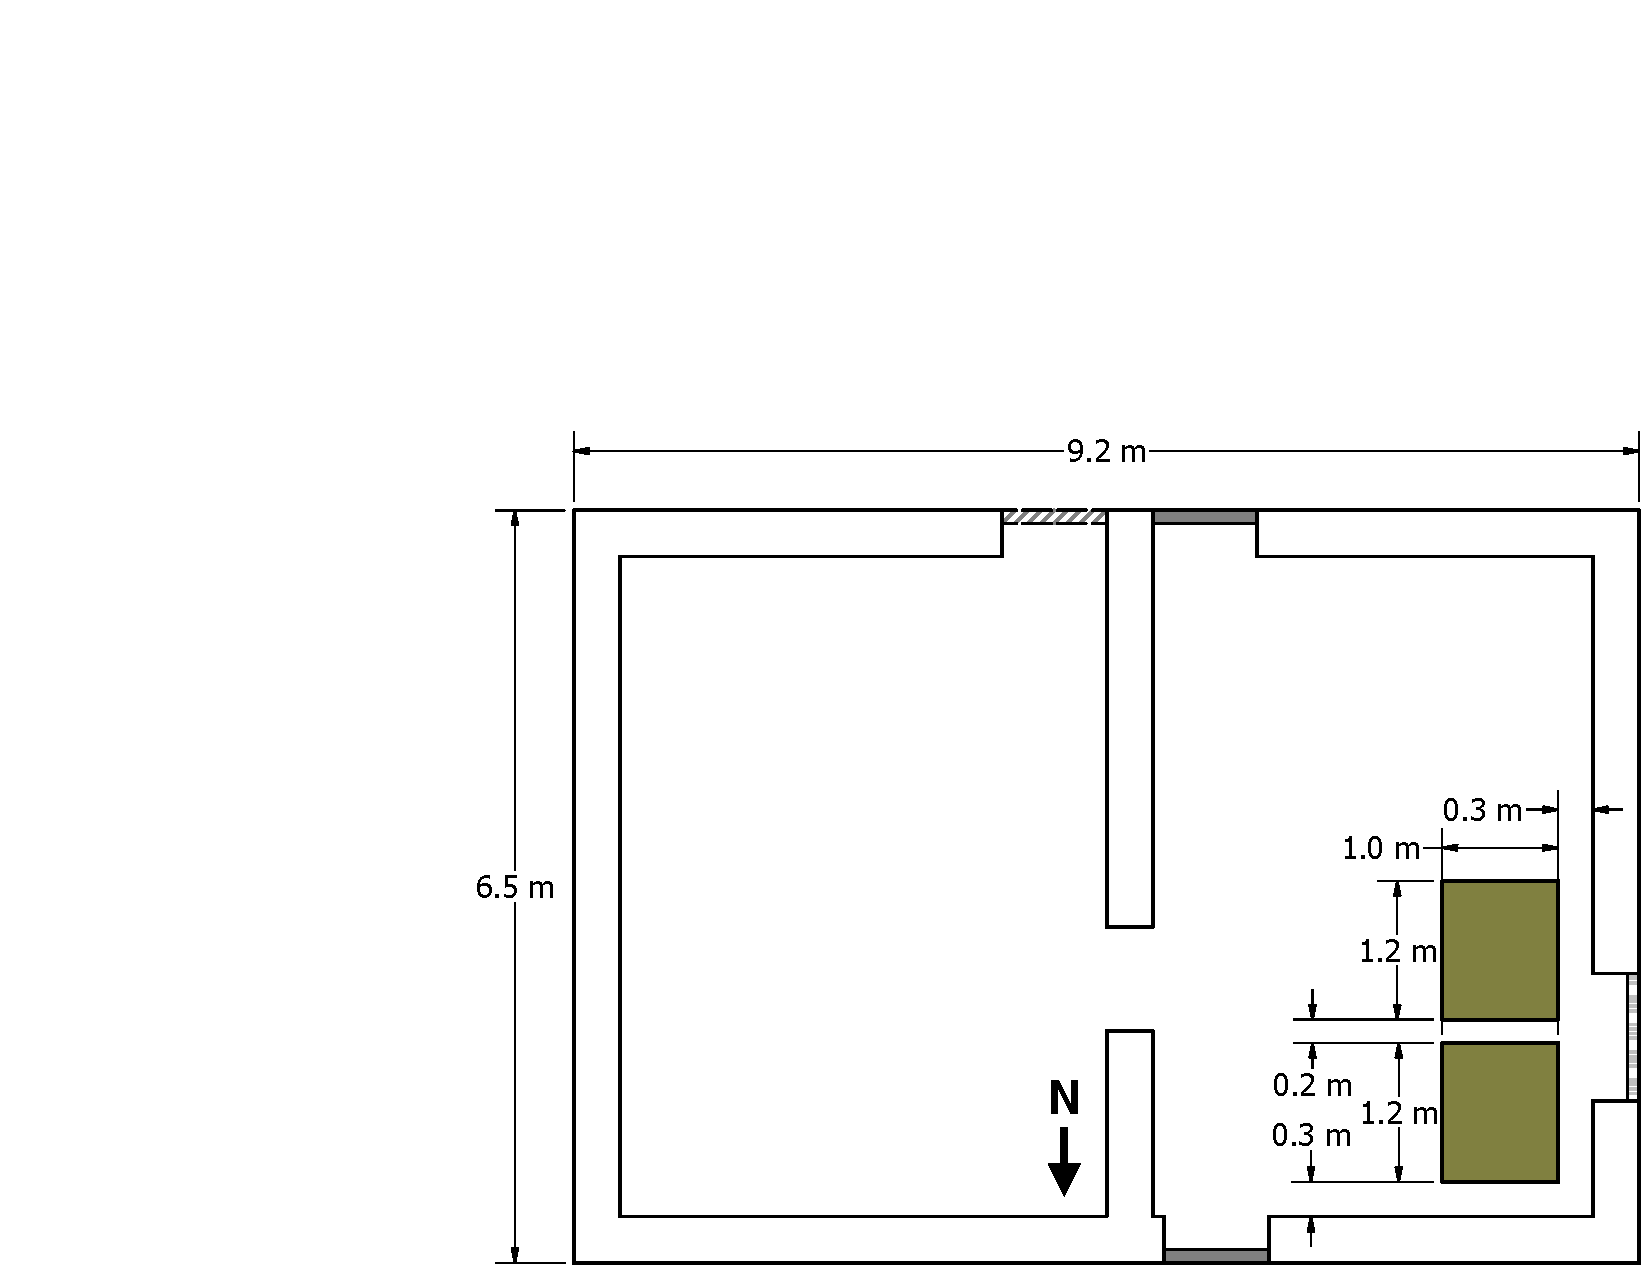
\includegraphics[width=\columnwidth]{../Figures/Floor_Plans/PDFs/West_Structure/DelCo_2012_West_Structure_Pallets}
	\caption{Burn Building Fuel Load}
	\label{fig:Burn_Building_Fuel_Load}
\end{figure}

Note that as the pallets burned away and the hot gas layer temperatures decreased, the steel shutters on the window to the burn room were opened and additional pallets were added. Pallets were added to the existing fuel locations until the flames from the piles reached the ceiling of the burn room again. Then, the shutters on the window were closed, and the temperature of the hot gas layer in the adjacent room was monitored in preparation for starting another gas cooling experiment.  The number of pallets added each time varied.

\clearpage

\subsection{Fire Suppression}
\label{sec:Fuel_Load_Fire_Suppression}

\subsubsection*{Single-Story Structure}
\label{sec:suppresion_single}

\subsubsection{Furniture Fuel Package}
\label{sec:fire_suppression_furniture_fuel}

The fuel load for test numbers 1 through 8 consisted of two sleeper sofas, two cushioned chairs, carpet, padding, and wood paneling along the southeast corner walls. An image of the fuel arrangement is shown in Figure~\ref{fig:Furniture_Fuel_Load}. The couches and chairs were set up to mimic a typical seating area with one couch against the south wall and one couch against the east wall, each positioned 0.9~m (36~in) away from the southeast corner. A chair was placed adjacent to each couch. The specific locations can be found in the dimensioned schematic, Figure~\ref{fig:Furniture_Fuel_Load_Dimensions}. In total, this fuel package contains approximately 336~kg (739~lb) of fuel consisting of wood, flexible polyurethane (PU), polyester (PE),and polypropylene (PP). Table~\ref{tab:Fire_Suppression_Fuel_Masses} provides a breakdown on the fuel composition for these experiments.

\begin{figure}[!ht]
	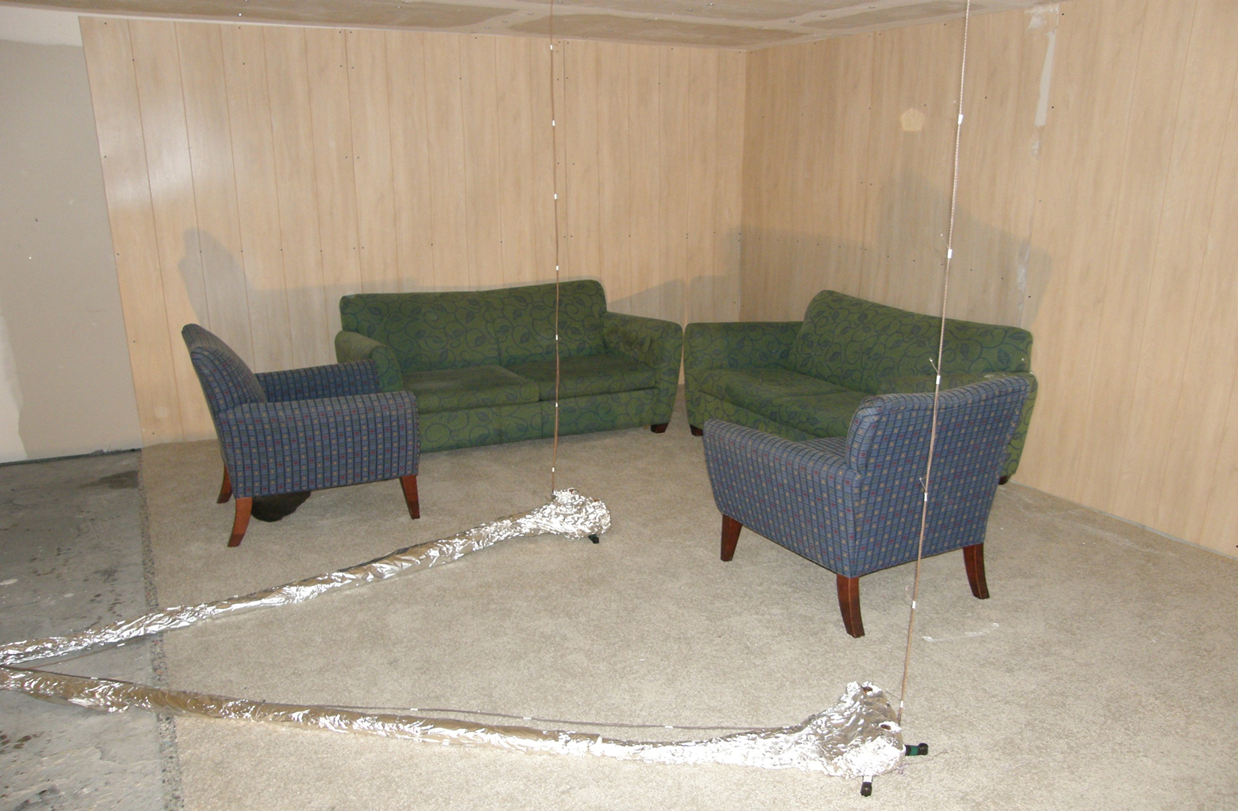
\includegraphics[width=.8\columnwidth]{../Figures/Pictures/Furniture_Fuel_Load}
	\caption{Furniture Fuel Load in Single-Story Structure}
	\label{fig:Furniture_Fuel_Load}
\end{figure}

\begin{figure}[!ht]
	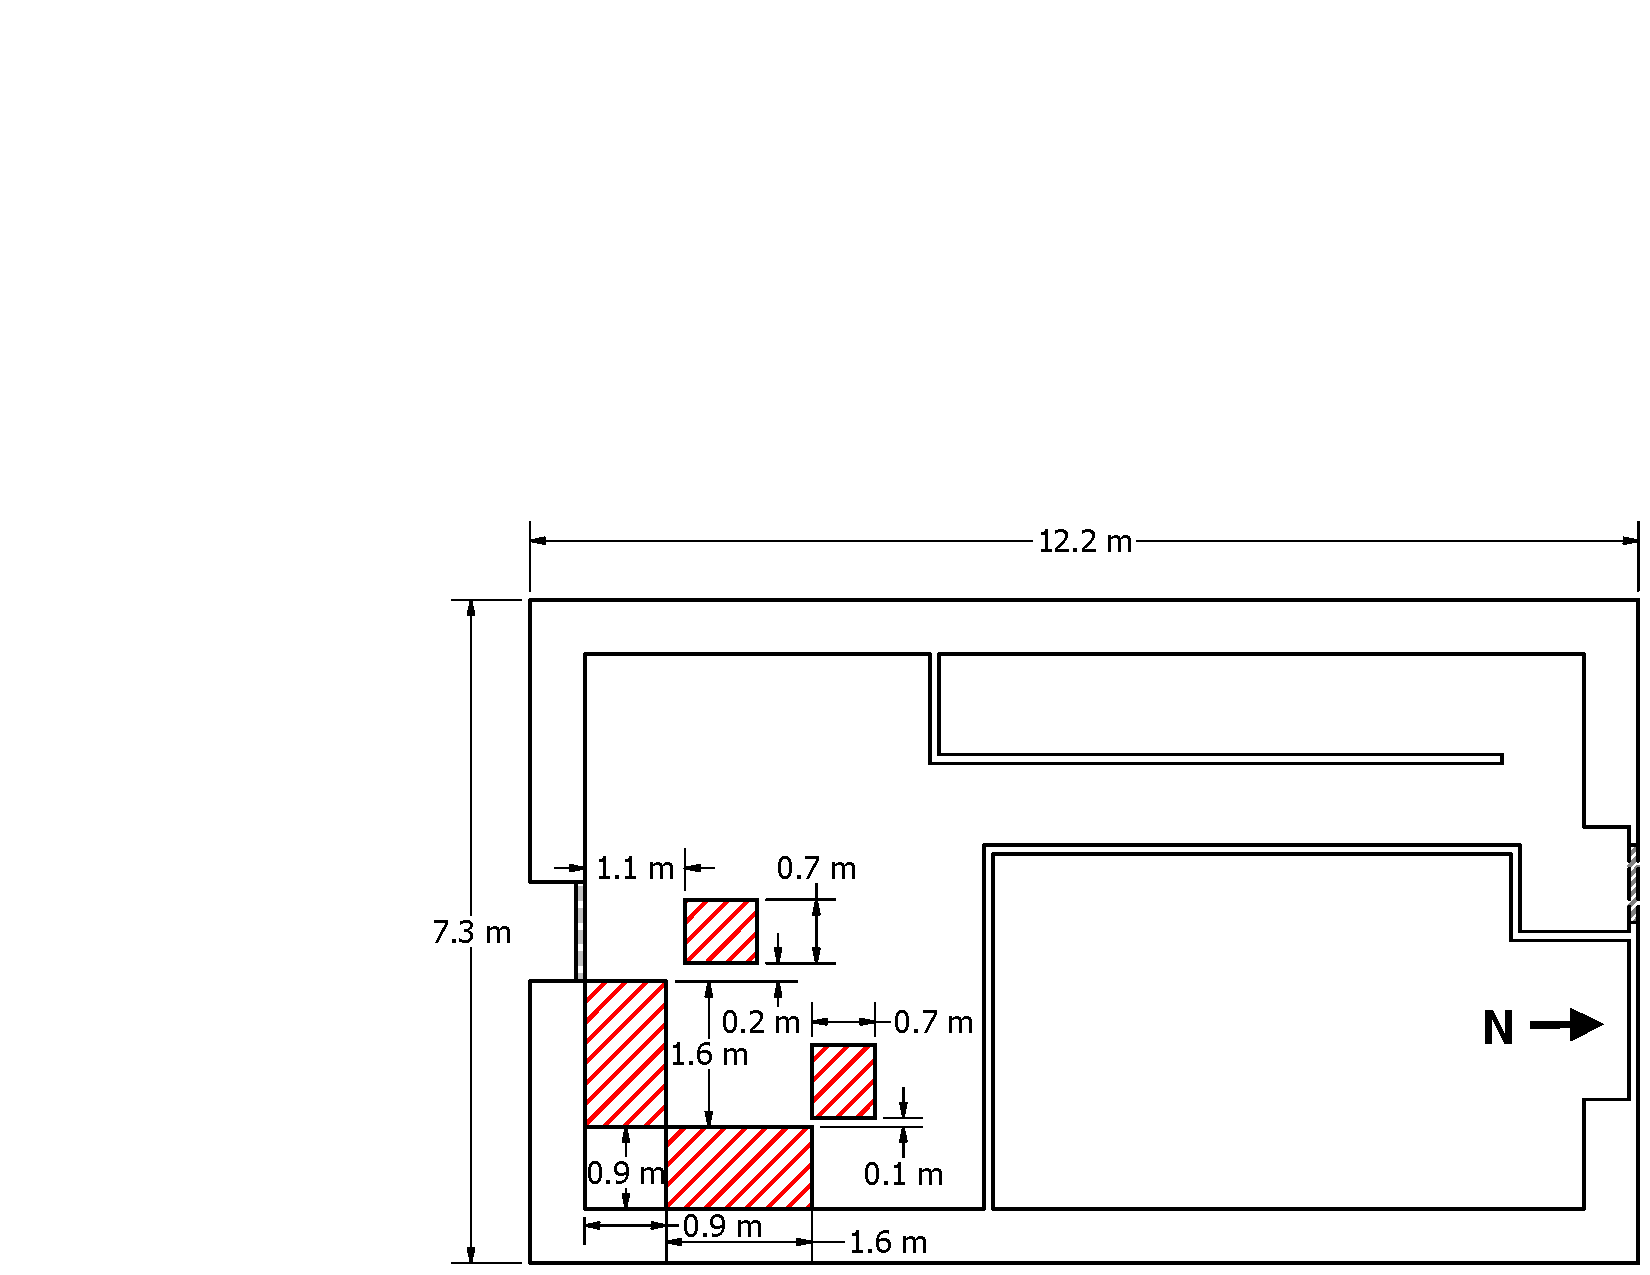
\includegraphics[width=.8\columnwidth]{../Figures/Floor_Plans/PDFs/East_Structure/DelCo_2012_East_Structure_Furniture}
	\caption{Furniture Fuel Load Dimensions in Single-Story Structure}
	\label{fig:Furniture_Fuel_Load_Dimensions}
\end{figure}

\begin{sidewaystable}[!ht]
	\centering
	\scriptsize
	\caption{Fire Suppression Furniture Fuel Package Description}
	\renewcommand{\tabcolsep}{1pt}
	\begin{tabular}{lllllcc}
		\toprule[1.5pt]
		Item               & Component		& Quantity		&  Material Description             			&  Dimensions (m)            	&  Mass (kg)  		& Total Mass (kg) \\
		\midrule
		2-seat Sofa        &				& 2				& 85~\% PU Foam, 15~\% PE Fiber, Wood Frame 	&  1.68 L X 0.90 D X 0.86 H  	&  72.4    			& 144.8 \\
		           	 	   & Mattress	    & 1 per sofa	& Cover: 52~\% PP, 48~\% PE,                    &  1.83 L X 1.21 W X 0.14 H     &  14.6             & \\
		           	 	   &                &               & Filling: 66~\% PE Pad, 34~\% PE Batting       &                               &                   & \\
			           	   & Cushion    	& 2 per sofa	& 85~\% PU Foam, 15~\% PE Fiber   				&  0.69 L X 0.58 D X 0.14 H  	&  2.2     			& \\
		Blue Chair         &				& 2				& 85~\% PU Foam, 15~\% PE Fiber, Wood Frame   	&  0.81 L X 0.75 D X 0.91 H  	&  17.4    			& 34.8 \\
		    			   & Cushion        & 1 per chair   & 85~\% PU Foam, 15~\% PE Fiber	    			&  0.51 L X 0.57 D X 0.14 H  	&  1.7    			& \\
		Blue/Green Chair   & 				& 2				& 85~\% PU Foam, 15~\% PE Fiber, Wood Frame     &  0.77 L X 0.71 D X 0.89 H  	&  16    			& 32 \\
		                   & Cushion    	& 1 per chair	& 85~\% PU Foam, 15~\% PE Fiber 		        &  0.55 L X 0.53 D X 0.15 H  	&  1.6    			& \\
		Paneling           &				& 8 panels		& Medium density fiberboard                     &  2.44 L X 1.22 W X 3.2~mm H   &  9    			& 72 \\
		Carpeting          &				& 22.3 m$^2$	& 100~\% Olefin fiber w/PP backing		     	&  3.68 L X 6.05 W  			&  32.2				& 32.2 \\
		Carpet Padding     &				& 22.3 m$^2$	& PU Foam                  	 				    &  3.68 L X 6.05 W X 11~mm H    &  19.8			    & 19.8 \\
		                   &                &               &                                               &                               & Total Mass        & 335.6 \\
		\bottomrule[1.25pt]
	\end{tabular}
	\label{tab:Fire_Suppression_Fuel_Masses}
\end{sidewaystable}

\subsubsection{Wood Fuel Package}
\label{sec:fire_suppression_pallet_fuel}

The fuel load for test numbers 9 through 12 consisted of one bale of hay, 12 pallets, 11.5 sheets of plywood on the walls, and the wood ``floor assembly''. Two stacks of pallets with hay were used as the first items ignited in each experiment. Each stack was composed of six pallets with a half bale of hay layered between the six pallets. Figure~\ref{fig:Wood_Fuel_Load} shows the pallets prior to ignition. The pallets and hay were weighed before each experiment, and the average mass of the two stacks of pallets and the bale of hay over the four experiments was 232.4~kg (511.3~lb).

\begin{figure}[!ht]
	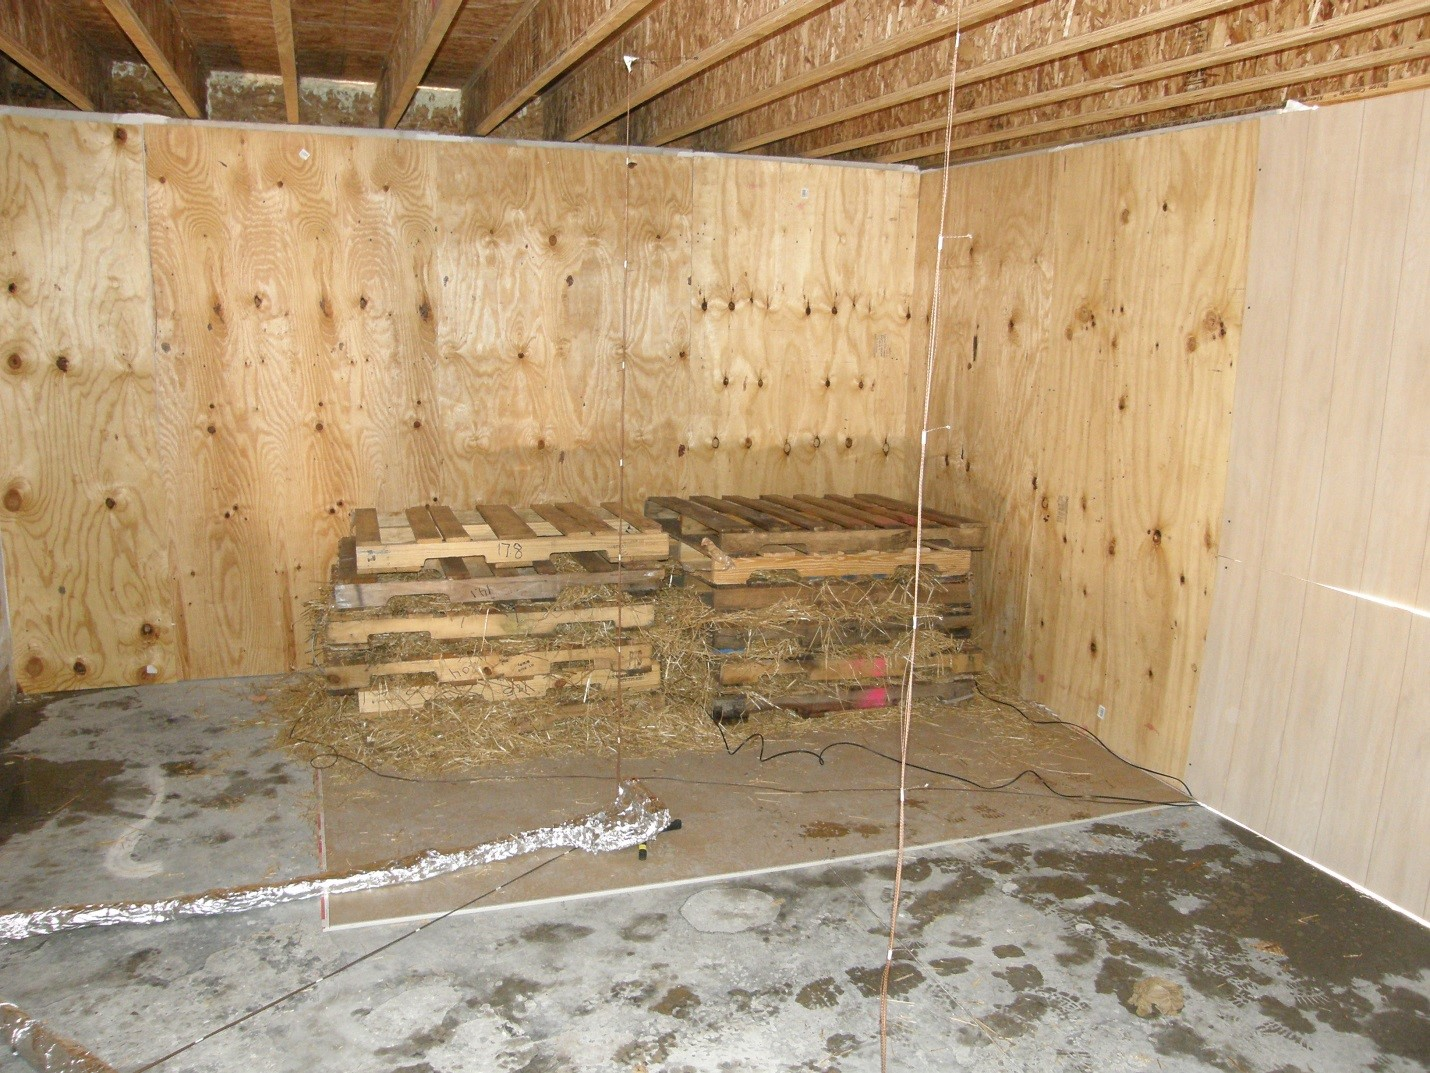
\includegraphics[width=0.65\columnwidth]{../Figures/Pictures/Wood_Fuel_Package}
	\caption{Southeast Corner of Burn Room with Wood Fuel Load}
	\label{fig:Wood_Fuel_Load}
\end{figure}

The pallet stacks were located 0.3~m (12~in) away from the east and south walls of the burn room (see Figure~\ref{fig:Wood_Fuel_Load_Dimensions}). The pallets were 1.2~m (48~in) long, 1.0~m (40~in) wide, and 123~mm (4.8~in) high. The stacks were spaced 150~mm (6~in) apart. One layer of 13~mm (0.5~in) thick gypsum board panels were laid on the concrete floor under the wood pallets to form a protective layer to minimize thermal damage to the concrete floor. The east and south walls of the burn room were covered with 15~mm (0.59~in) thick sheets of plywood.  The wood ``flooring assembly'', composed of 12 TJIs and nine sheets of oriented strand board (OSB), served as the ceiling of the burn room. The open doorway to the burn room on the south side was covered with a 2.4~m (8~ft) tall by 1.2~m (4~ft) wide piece of medium density fiberboard paneling that was 5~mm (0.19~in) thick.

\begin{figure}[!ht]
	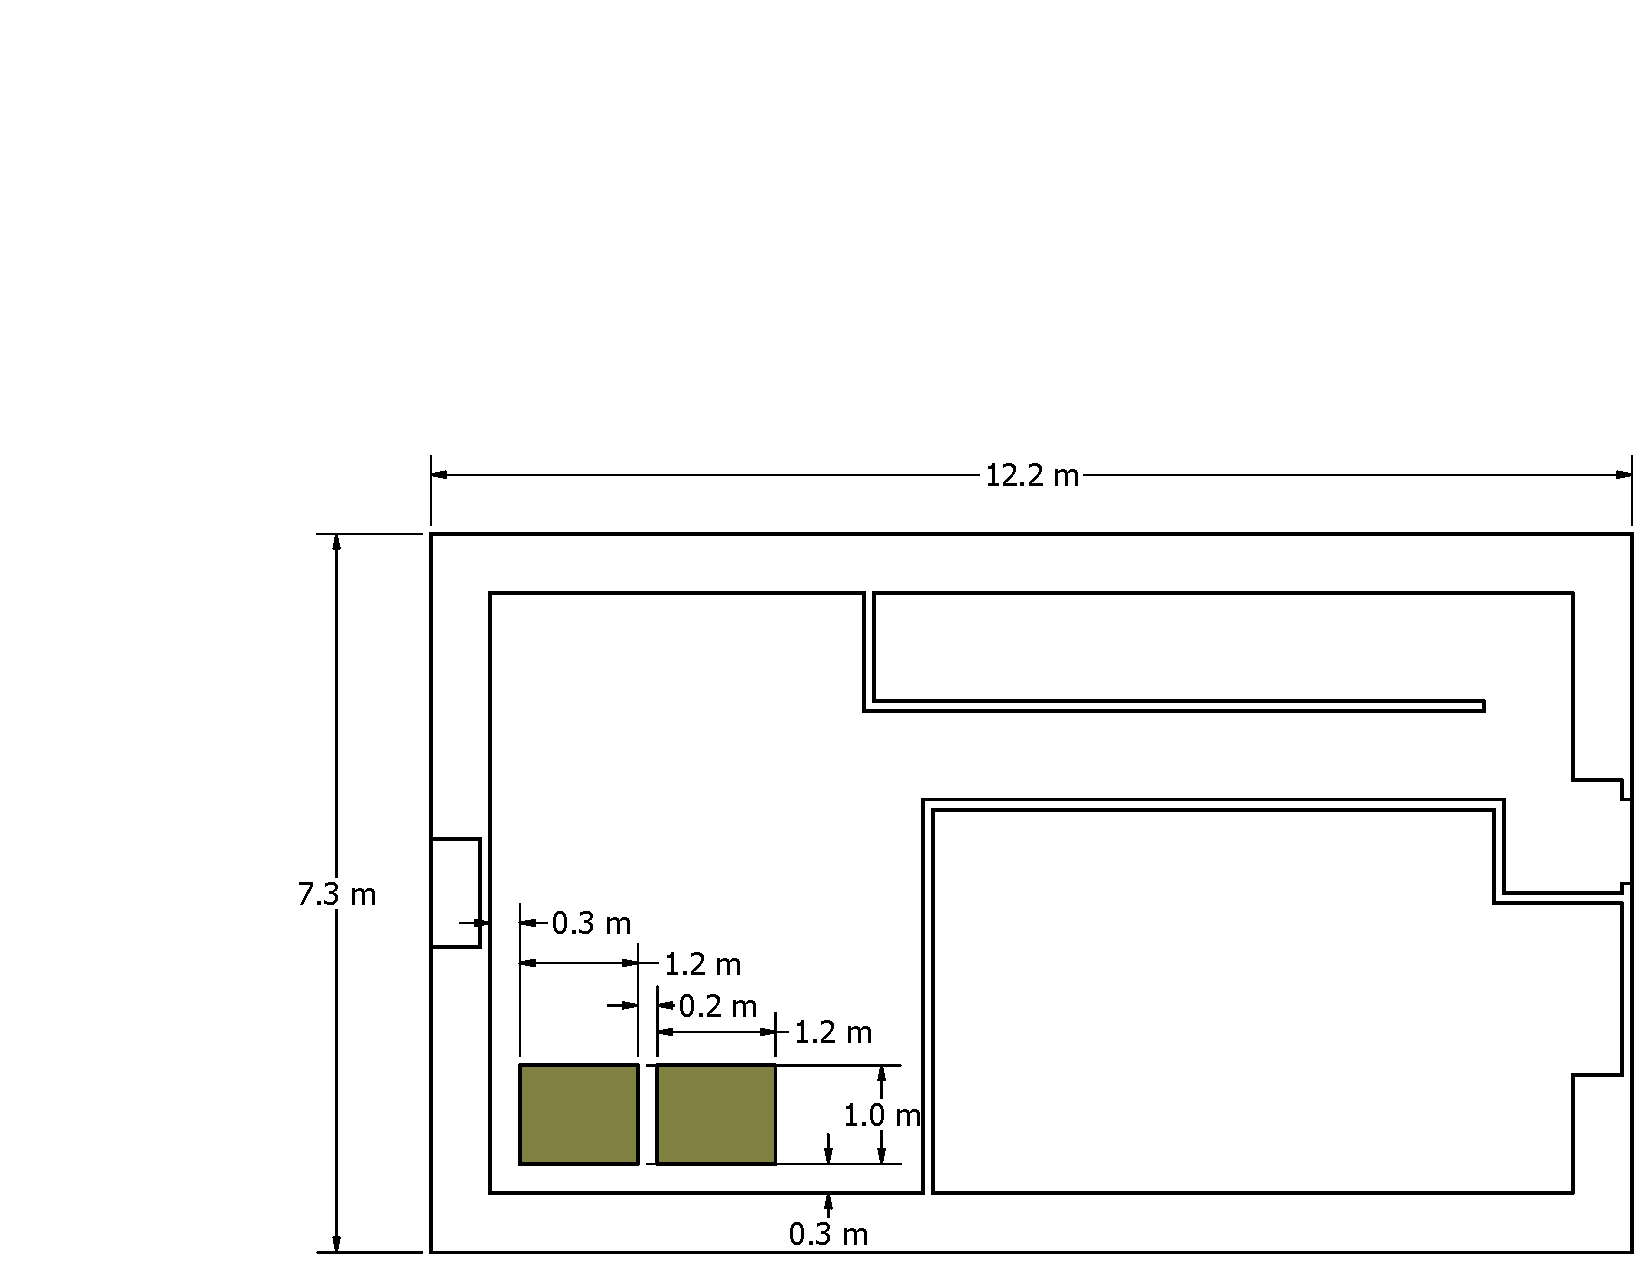
\includegraphics[width=.8\columnwidth]{../Figures/Floor_Plans/PDFs/East_Structure/DelCo_2012_East_Structure_Pallets}
	\caption{Wood Fuel Load Dimensions in Single-Story Structure}
	\label{fig:Wood_Fuel_Load_Dimensions}
\end{figure}


\subsubsection*{Two-Story Structure}
\label{sec:suppresion_two}

In June of 2015, the larger compartment experiments, experiments 13 through 20, were conducted in the lower level of the two-story structure.  Two different fuel packages were utilized, the difference between the furniture fuel package used for experiments 13 and 14, and the furniture and pallet fuel package used in experiments 15 through 20 was the addition of two stacks of pallets.   

\subsubsection{Furniture Fuel Package}
\label{sec:fire_suppression_furniture_fuel_2}

The fuel load for two of the experiments consisted of three sofas with an average mass of 48.7~kg; 51.4~m$^2$ (559~ft$^2$) of carpet and padding; and approximately 38 sheets of OSB paneling with dimensions 16~mm (0.63~in) x 1.2~m (4~ft) x 2.4~m (8~ft) along the east, west, and south walls and ceiling. The three couches were aligned along the west wall and spaced 1.2~m (4~ft) apart. The specific locations can be found in the dimensioned schematic Figure~\ref{fig:furniture_2story}. In total, this fuel package was composed of wood, flexible polyurethane (PU), polyester (PE), and polypropylene (PP).

\begin{figure}[!ht]
	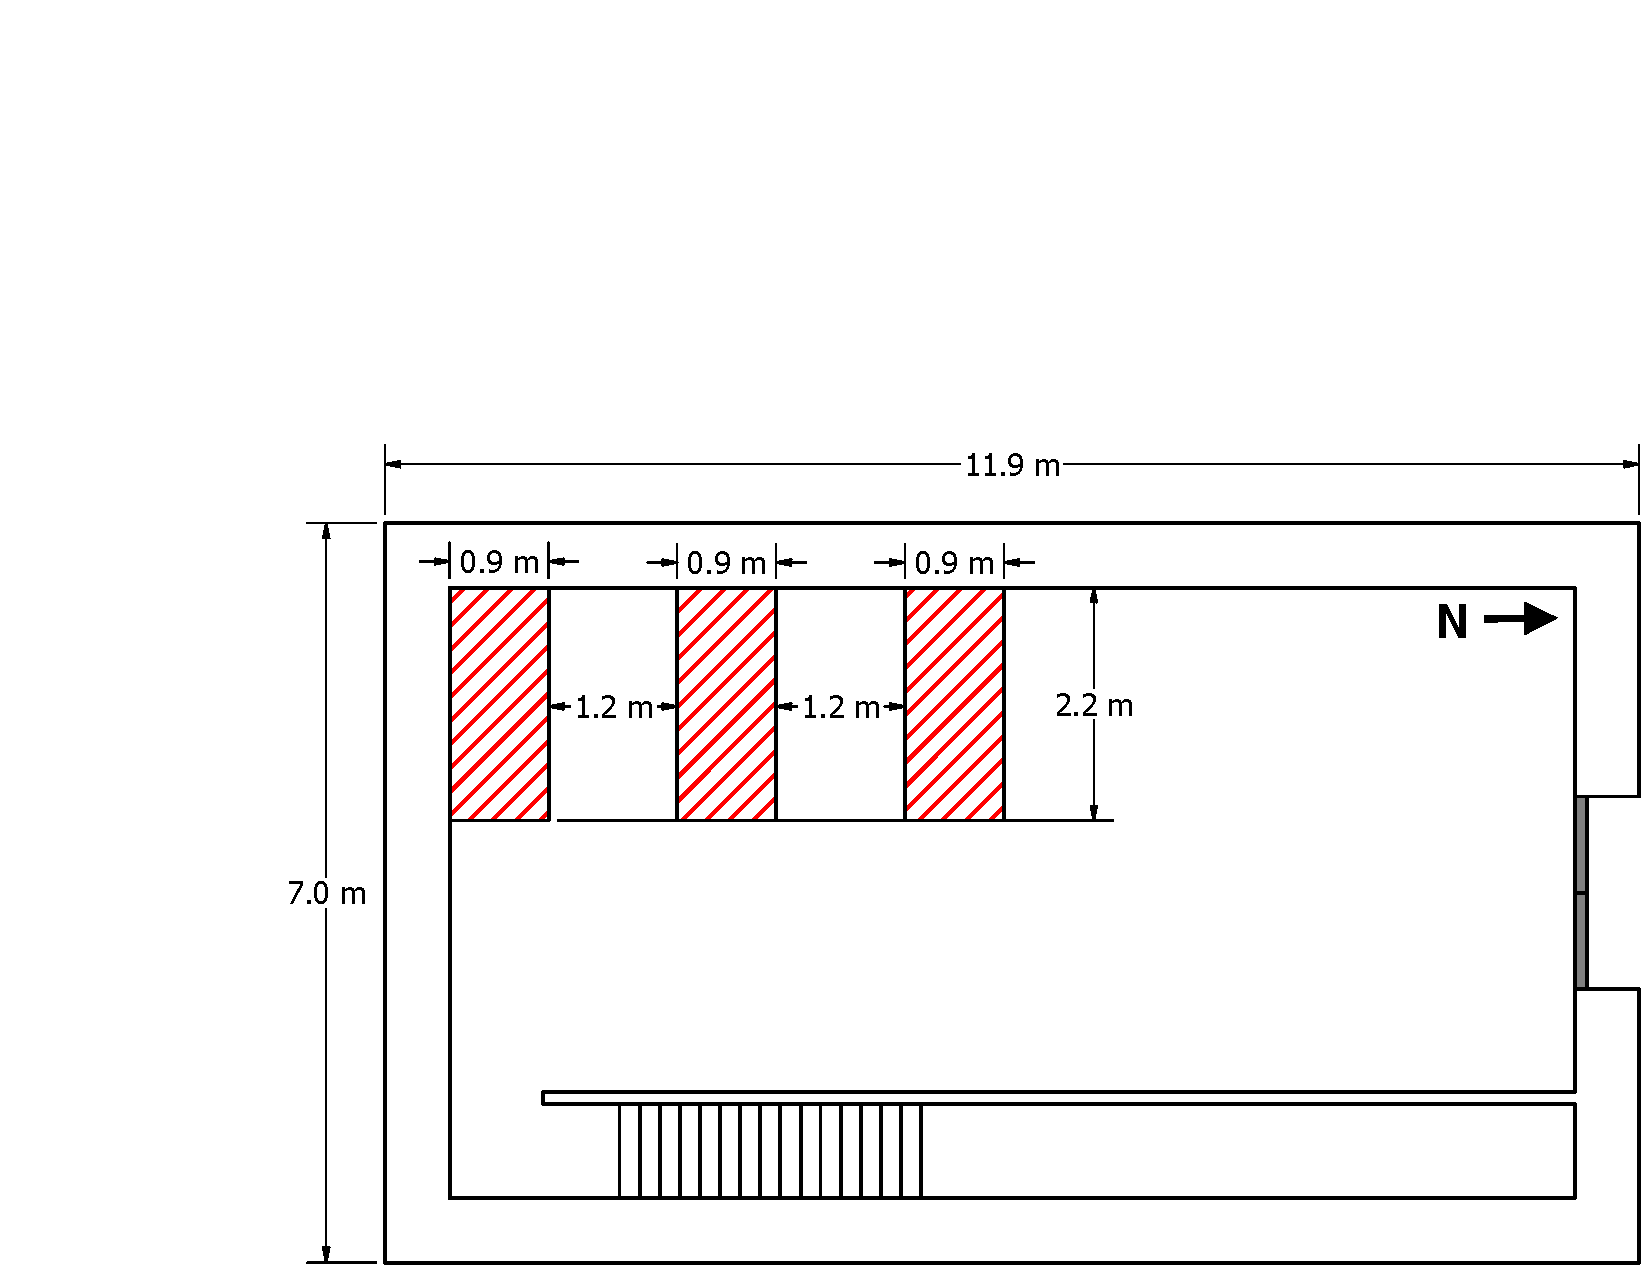
\includegraphics[width=\columnwidth]{../../DelCo_2014_2015/Drawings/PDFs/CAFS/West_Structure_1st_Floor_Furniture_Only}
	\caption{Furniture Fuel Load Dimensions in First Floor of Two-Story Structure}
	\label{fig:furniture_2story}
\end{figure}

\subsubsection{Furniture and Pallet Fuel Package}
\label{sec:fire_suppression_combo_fuel_2}

In June 2015, two stacks of pallets were added to the fuel load consisting of three sofas; OSB lining on the ceiling and walls; and the polypropylene carpeting over polyurethane foam padding. Each stack had 10 pallets and an approximate mass of 175~kg (386~lb). Hay from bales averaging a mass of 12~kg (26~lb) was added for ignition purposes. The specific locations of the fuel load's contents can be found in the dimensioned schematic Figure~\ref{fig:pallet_furniture_2story}.

\begin{figure}[!ht]
	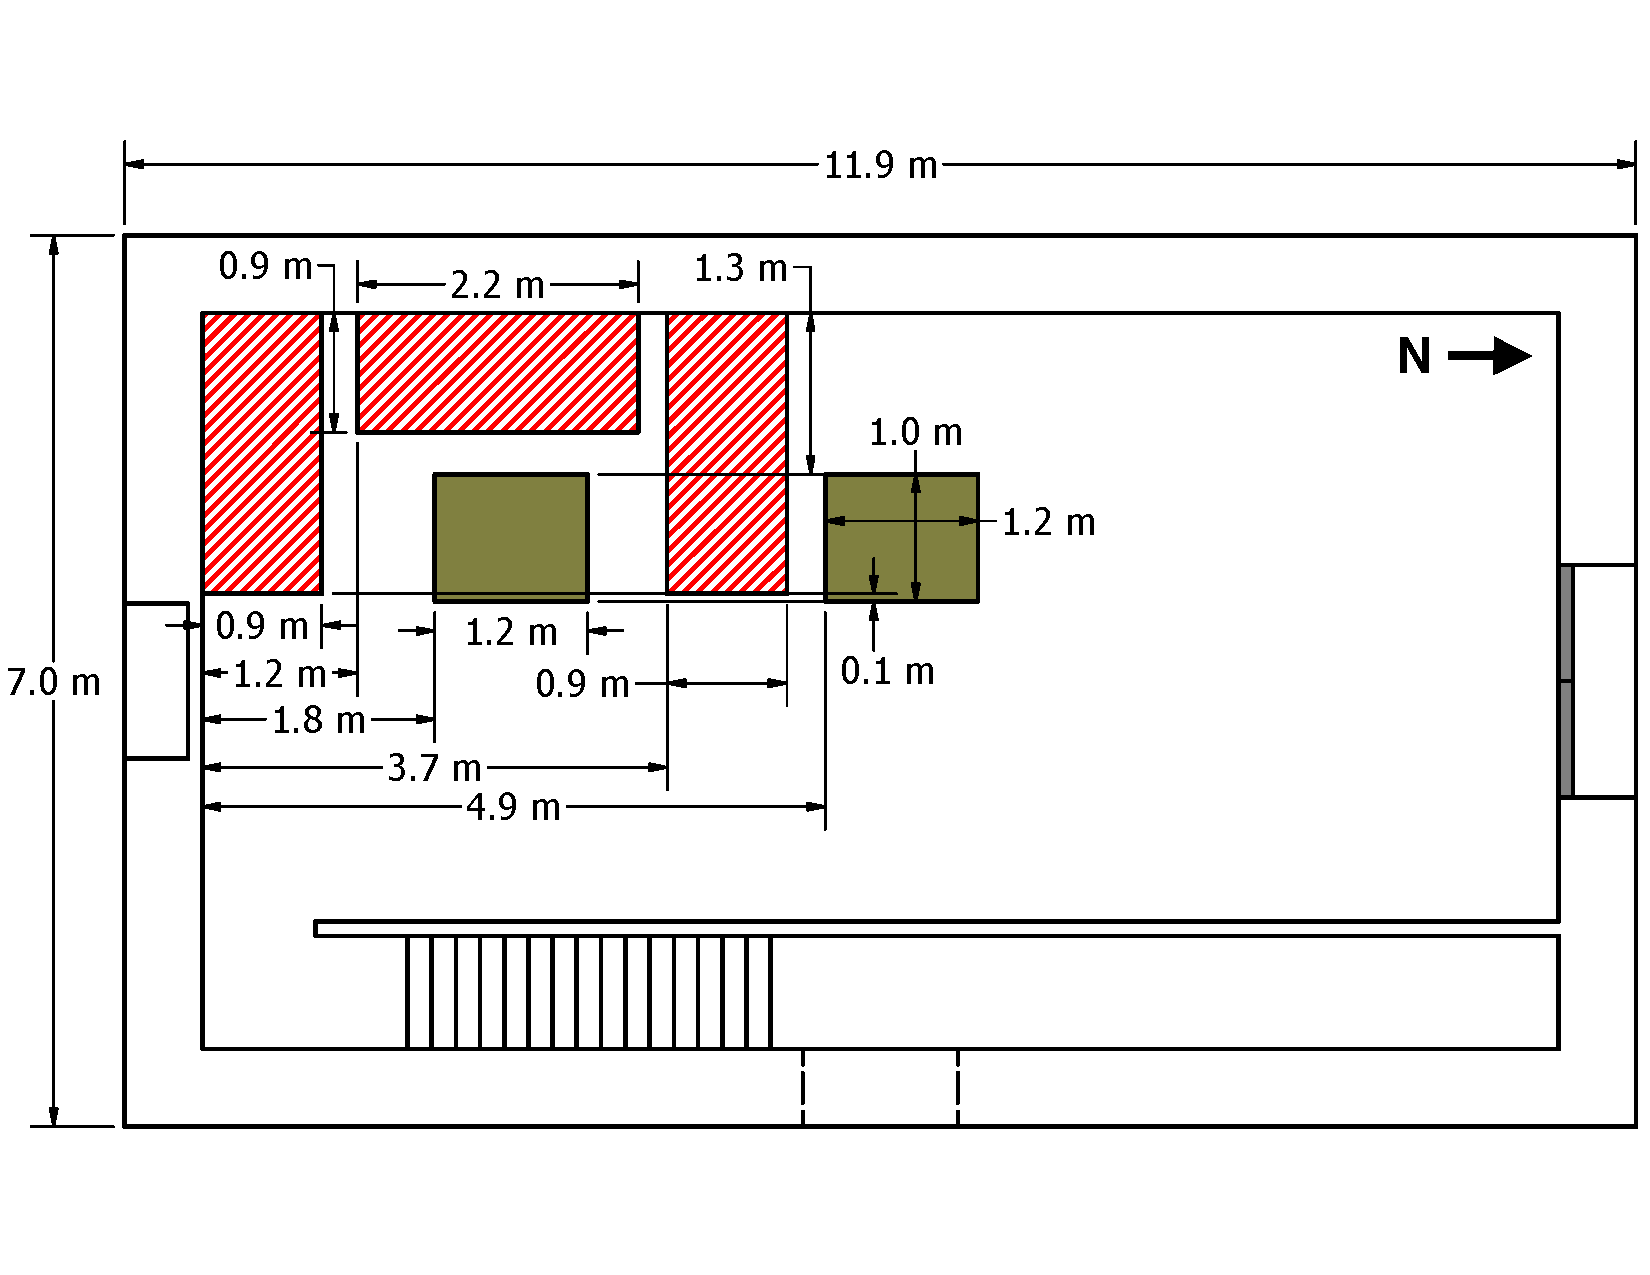
\includegraphics[width=\columnwidth]{../../DelCo_2014_2015/Drawings/PDFs/CAFS/West_Structure_1st_Floor_Furniture_Pallets}
	\caption{Furniture and Pallet Fuel Load Dimensions in First Floor of Two-Story Structure}
	\label{fig:pallet_furniture_2story}
\end{figure}

\chapter{Experiments and Results}
\label{chap:Experiments_and_Results}

The following results are arranged in the order that the experiments were conducted. For the fire suppression experiments, the fuel load and resulting fire hazard were intended to increase as the different structures and fuel packages were utilized.  

\section{Spray Density}
\label{sec:Spray_Density}

Spray density experiments were conducted by placing 0.23~m$^2$ (2.5~ft$^2$) interlocking water collection pans across the floor surface area of the burn rooms within each structure (see Figure~\ref{fig:water_buckets}). The depth of the pans was 0.3 m (1 ft).  Water or CAF was flowed for a specified duration or until it appeared that a pan was filled.  Upon completion of the test, the bins were removed from the structure. Then, each bin was weighed to quantify the impact of nozzle location and spray pattern. Thirty-three spray density tests were conducted: 21 in the burn building used for the gas cooling tests and 12 in the single-story structure used for the fire suppression experiments. The interior of the fire room in the single-story structure was sheathed in plastic for the spray density tests to protect the gypsum board from being soaked with water prior to the fire suppression experiments. The flow rate for each test was 120~gpm for water and 120~gpm plus 60~cfm air for CAF. Tables~\ref{tab:spray_density_tests} and \ref{tab:spray_density_tests2} provide an overview of each experiment. In the table, ``GC'' stands for the gas cooling experiments, and ``SE'' stands for the suppression experiments. For all experiments, 30~m (100~ft) of 4.45~cm (1.75~in) diameter hoseline connected to a ``blitz-fire'' monitor with a Metro 1 nozzle was used.

\begin{figure}[!ht]
	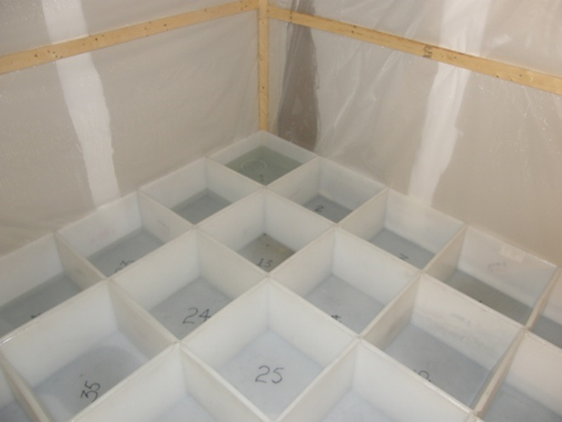
\includegraphics[width=.5\columnwidth]{../Figures/Pictures/Water Tests Bins.png}
	\caption{Interlocking collecting bins used to capture suppression agent during spray density tests}
	\label{fig:water_buckets}
\end{figure}

For the spray density tests listed in Table~\ref{tab:spray_density_tests}, the ``mid'' position had the centerline of the stream aimed at 2.44~m (8~ft) south of the north wall and 2.13~m (7~ft) west of the east wall in the concrete burn building.  The ``back'' position had the centerline of the stream aimed at 3.36~m (11~ft) south of the north wall and 2.13~m (7~ft) west of the east wall in the concrete burn building. Figure~\ref{fig:stream_position} shows the streams from the monitor nozzle for the middle and back positions. From the images, the qualitative difference of the nozzle positions can be observed.  When the stream is in the middle position, after the stream hits the ceiling, the impact region is relatively narrow with the majority of the water hitting the walls of the corner opposite the nozzle position.  When the nozzle is in the back position, the stream hits the ceiling at a much steeper angle and the droplets from the broken stream have a broader distribution throughout the room.   

\begin{figure}[!ht]
	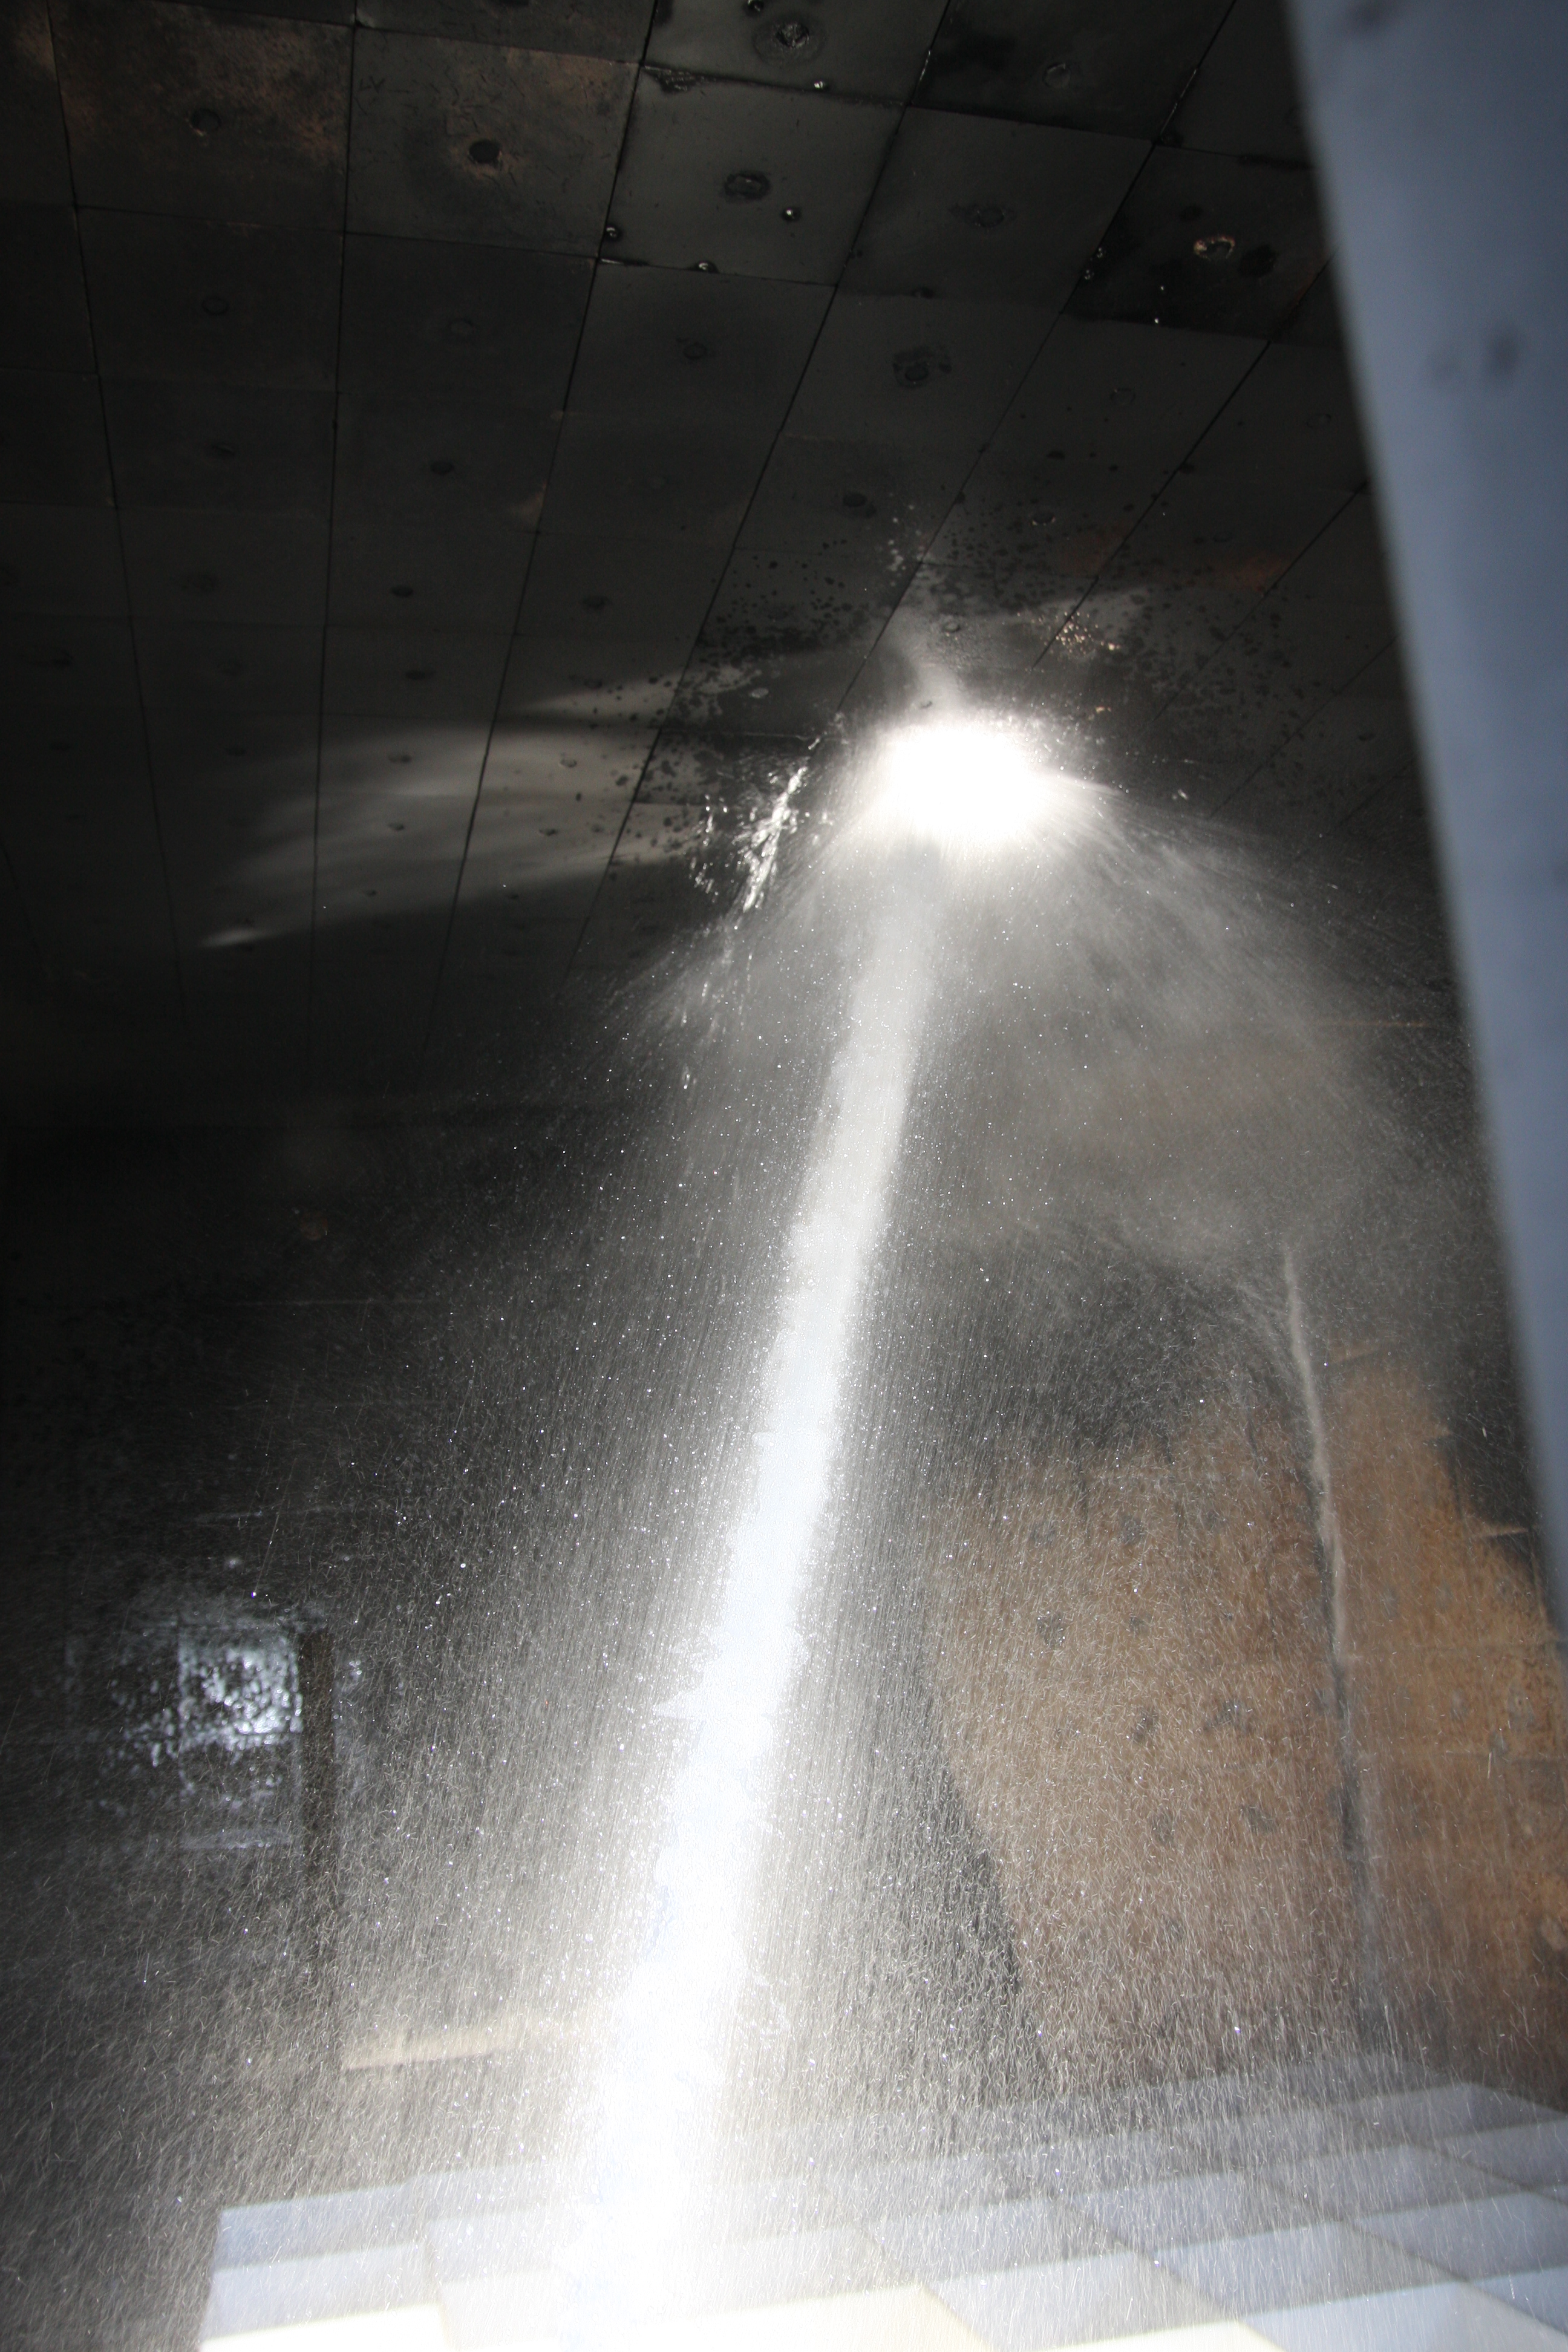
\includegraphics[width=.4\columnwidth]{../Figures/Pictures/Straight_Mid_BB}
	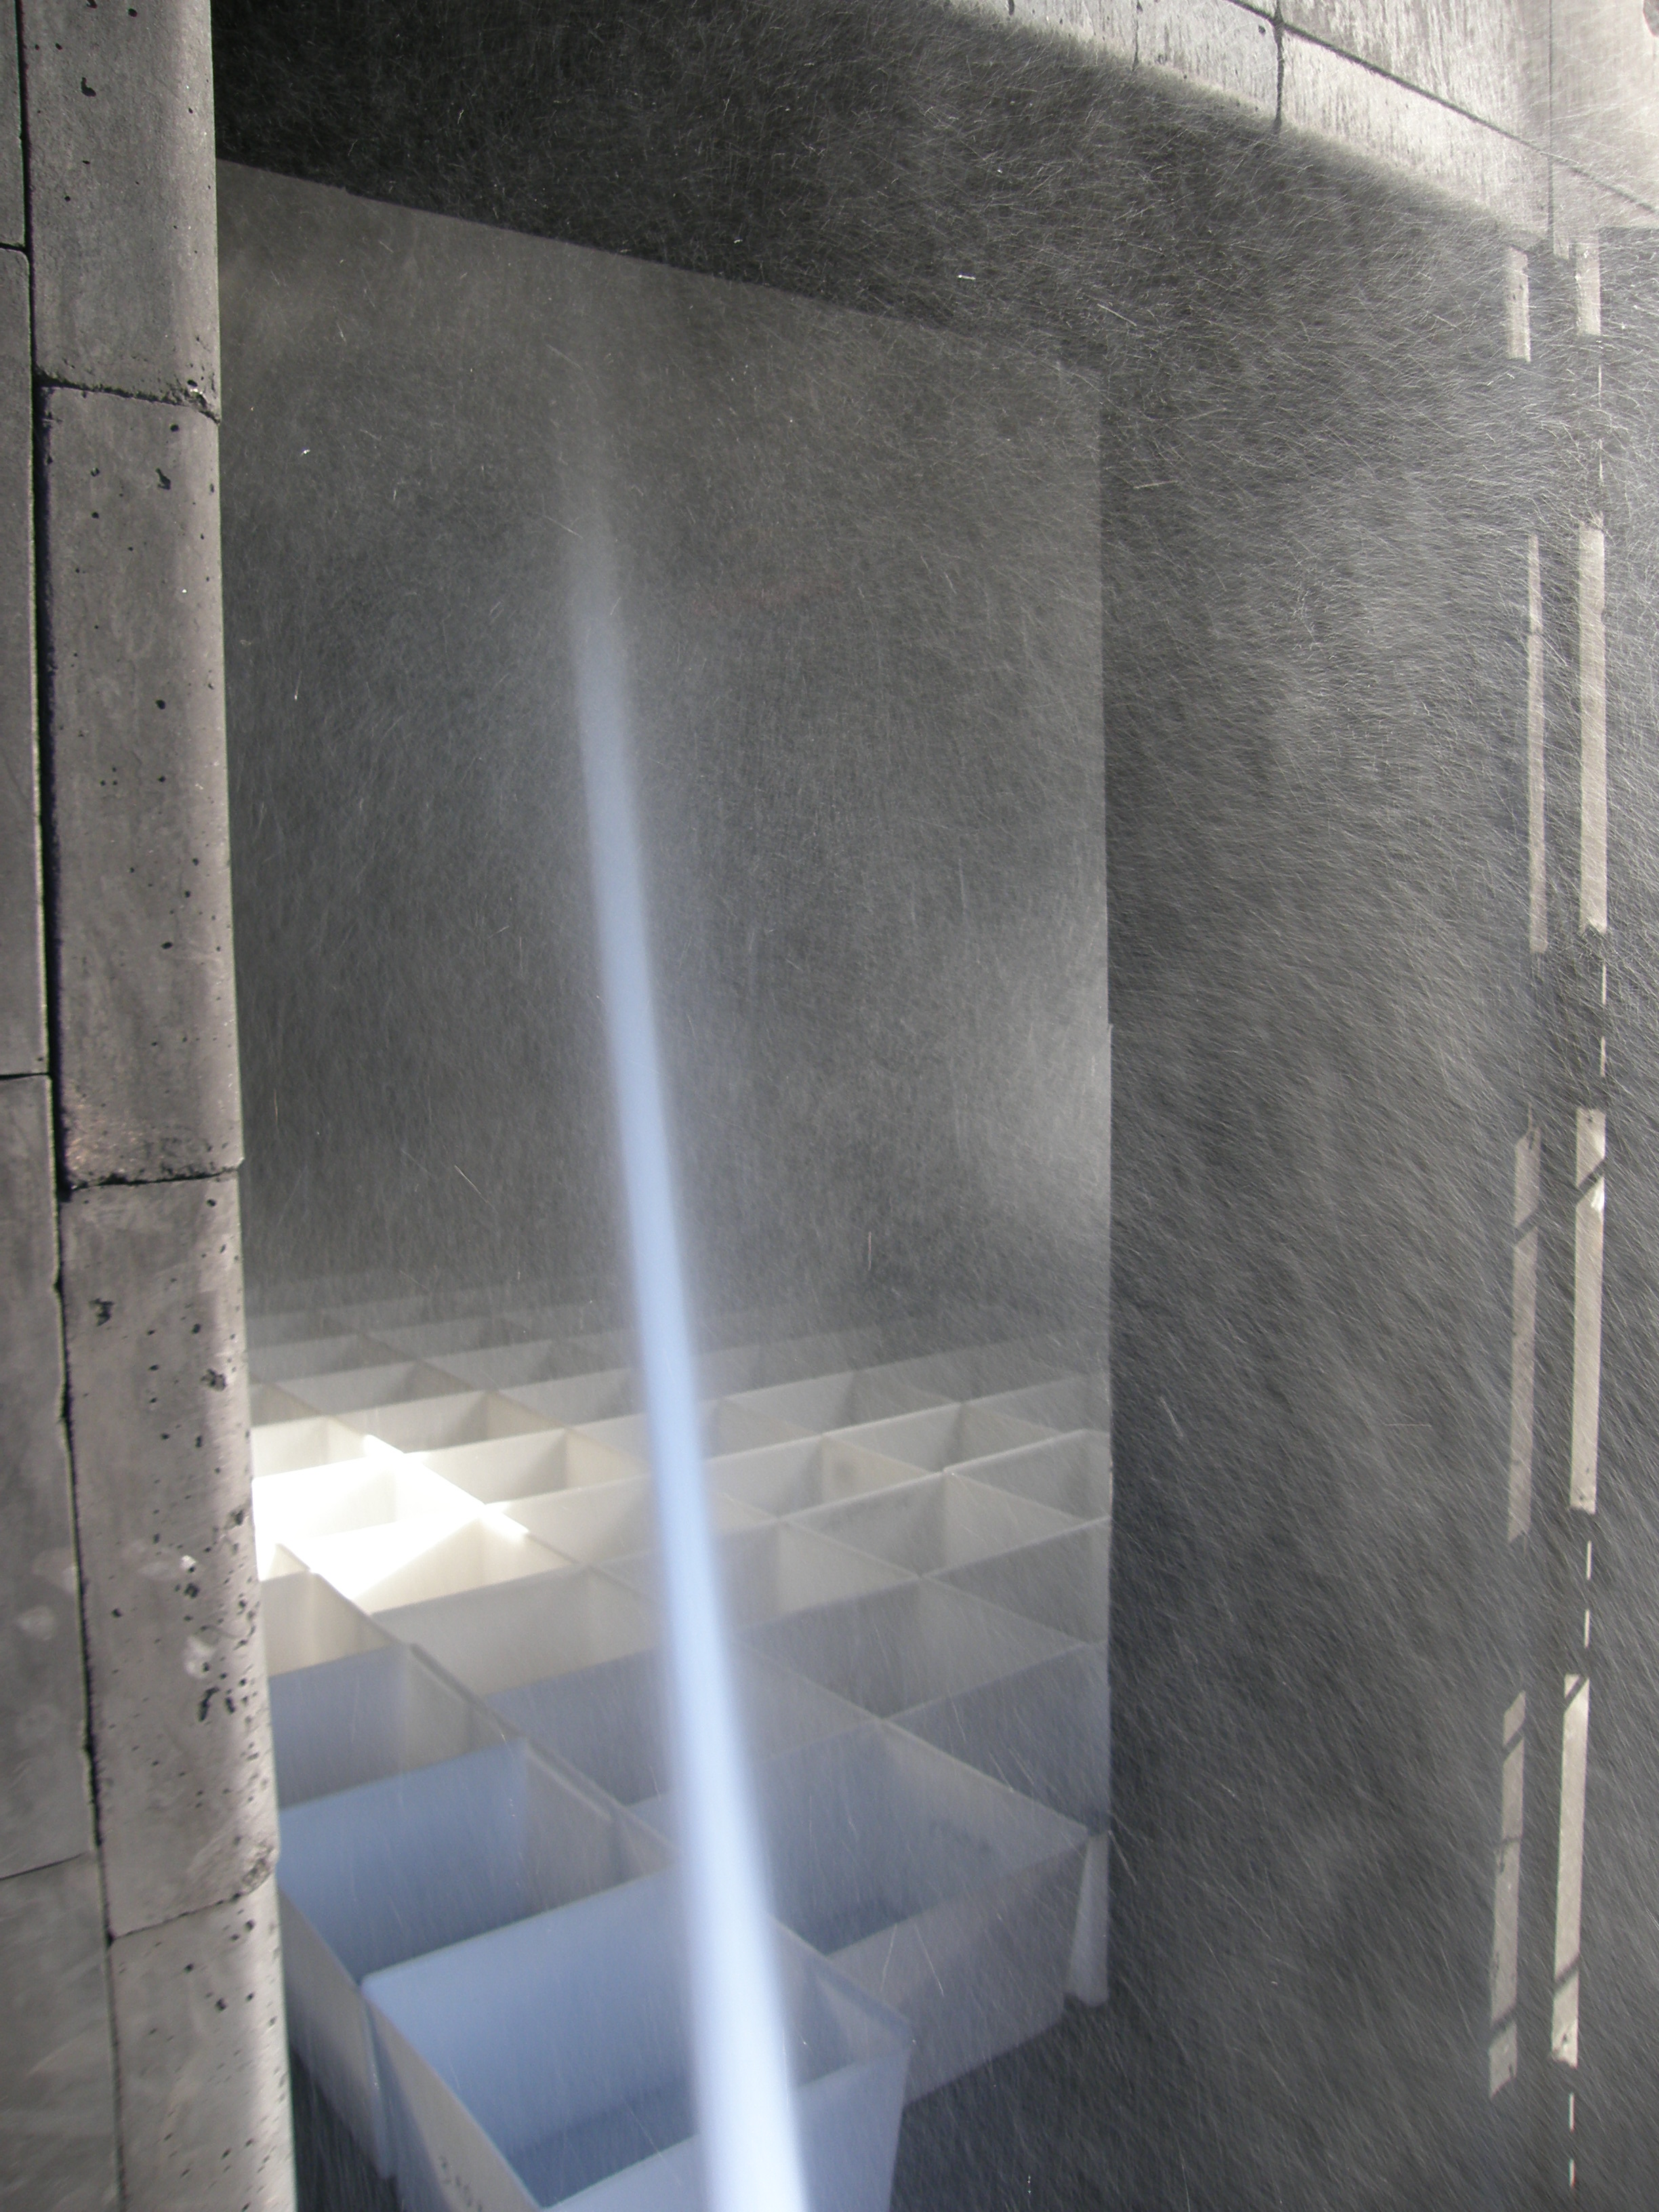
\includegraphics[width=.4\columnwidth]{../Figures/Pictures/Straight_Back_BB}
	\caption[Middle and Back Stream Positions During Spray Density Tests]{Middle (left) and Back (right) Stream Positions During Spray Density Tests}
	\label{fig:stream_position}
\end{figure}

\begin{table}[!ht]
\footnotesize
\centering
\captionof{table}{Spray Density Test Matrix for Gas Cooling Experiments}\label{tab:spray_density_tests}
\begin{tabular}{lllll}
\toprule[1.5pt]
Test \#    &  Duration (s)  & Agent  &  Pattern            	& Nozzle Position  \\
\midrule
GC1        &  15            & Water  &  Straight Stream    	& Back             \\
GC2        &  23            & Water  &  Straight Stream    	& Back             \\
GC3        &  15            & Water  &  Straight Stream    	& Mid              \\
GC4        &  15            & Water  &  Straight Stream    	& Mid              \\
GC5        &  20            & Water  &  Straight Stream 	& Mid              \\
GC6        &  21            & Water  &  Narrow Fog   		& Mid              \\
GC7        &  20            & Water  &  Narrow Fog   		& Mid              \\
GC8        &  22            & Water  &  Narrow Fog   		& Back             \\
GC9        &  24            & Water  &  Narrow Fog   		& Back             \\
GC10       &  20            & Water  &  Solid Stream       	& Back             \\
GC11       &  22            & Water  &  Solid Stream       	& Back             \\
GC12       &  15            & CAF    &  Solid Stream       	& Back             \\
GC13       &  10            & CAF    &  Solid Stream       	& Mid              \\
GC14       &  15            & CAF    &  Solid Stream       	& Back             \\
GC15       &  20            & CAF    &  Solid Stream       	& Mid              \\
GC16       &  15            & CAF    &  Narrow Fog   		& Mid              \\
GC17       &  20            & CAF    &  Straight Stream    	& Mid             \\
GC18       &  10            & CAF    &  Straight Stream    	& Mid             \\
GC19       &  15            & CAF    &  Narrow Fog   		& Back             \\
GC20       &  15            & CAF    &  Narrow Fog   		& Back             \\
GC21       &  15            & CAF    &  Straight Stream    	& Back             \\
\bottomrule[1.25pt]
\end{tabular}\par
\end{table}
For the fire suppression spray density experiments, Table~\ref{tab:spray_density_tests2}, the hallway position had the center of the stream aimed at the ceiling of the burn room, 2.14~m (7~ft) north of the south wall and 1.53~m (5~ft) east of the west wall. The fire room position had the center of the stream aimed at the ceiling of the burn room, 2.14~m (7~ft) north of the south wall and 3.05~m (10~ft) west of the east wall.

\begin{table}[!ht]
\footnotesize
\centering
\captionof{table}{Spray Density Test Matrix for Fire Suppression Experiments}\label{tab:spray_density_tests2}
\begin{tabular}{lllll}
\toprule[1.5pt]
Test \#    & Duration (s)  & Agent  &  Pattern            & Nozzle Location  	\\
\midrule
SE1        & 7             & Water  &  Straight Stream    &    Fire Room          \\
SE2        & 18            & Water  &  Straight Stream    &    Fire Room          \\
SE3        & 19            & Water  &  Straight Stream    &    Fire Room          \\
SE4        & 21            & Water  &  Straight Stream    &    Fire Room          \\
SE5        & 22            & Water  &  Narrow Fog  		  &    Fire Room          \\
SE6        & 19            & Water  &  Narrow Fog   	  &    Fire Room          \\
SE7        & 16            & Water  &  Solid Stream       &    Fire Room          \\
SE8        & 17            & Water  &  Solid Stream       &    Hallway            \\
SE9        & 15            & Water  &  Narrow Fog   	  &    Hallway            \\
SE10       & 16            & Water  &  Narrow Fog   	  &    Hallway            \\
SE11       & 16            & Water  &  Straight Stream    &    Hallway            \\
SE12       & 16            & Water  &  Straight Stream    &    Hallway            \\
\bottomrule[1.25pt]
\end{tabular}\par
\end{table}

\clearpage

After weighing each of the bins, the mass of water (kg) in each bin was plotted by position to visualize the spray distribution. Figure~\ref{fig:Burn_Building_Test_1} shows that with a straight stream in the back position, the majority of the water accumulated along the north and east walls of the gas cooling room within the burn building (see Figure~\ref{fig:Delaware_County,_PA_Burn_Building_Layout}). Figure~\ref{fig:Burn_Building_Test_7} shows the results from a fog stream, where the distribution of water is far more dispersed around the gas cooling room. The remainder of the burn building spray density figures are included in Appendix~\ref{app:spray_density}.

\begin{figure}[!ht]
	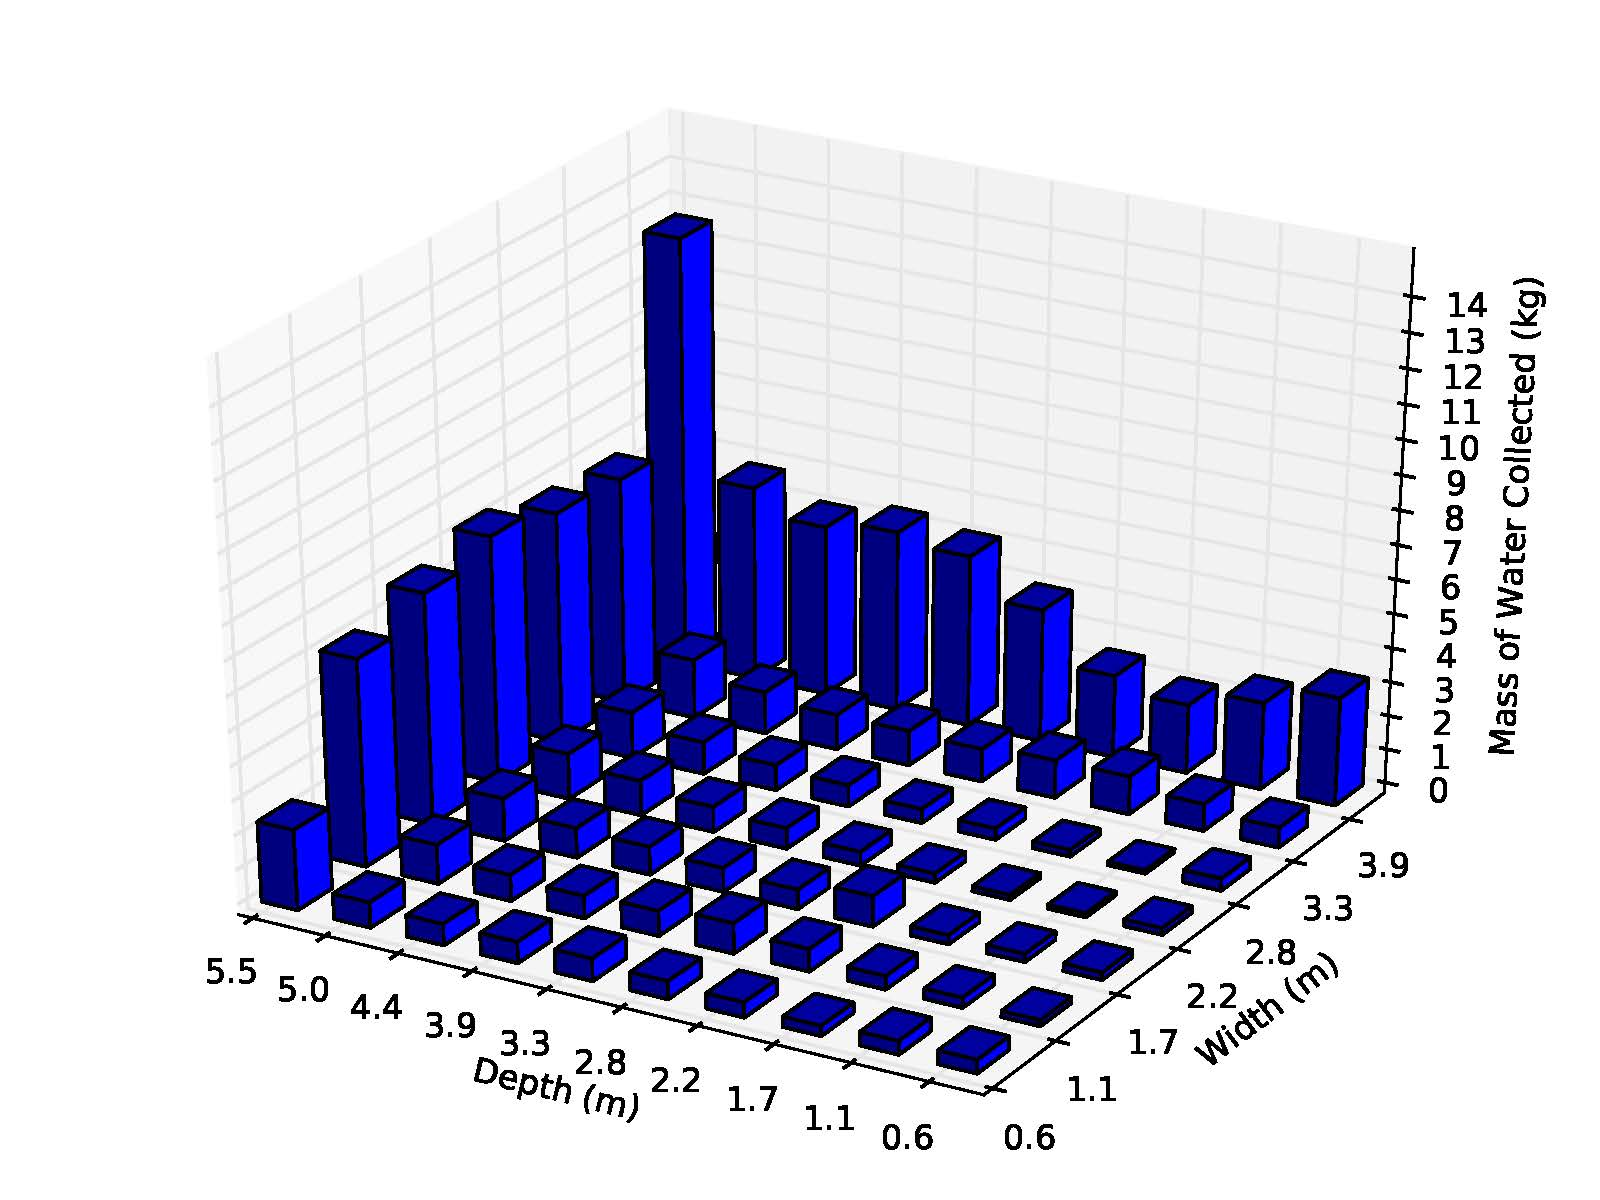
\includegraphics[width=4in]{../Figures/Bars/BB1}
	\caption{Gas Cooling Spray Density Test 1, Straight Stream/Back Nozzle Position}
	\label{fig:Burn_Building_Test_1}
\end{figure}

\begin{figure}[!ht]
	\includegraphics[width=4in]{../Figures/Bars/BB7}
	\caption{Gas Cooling Spray Density Test 7, Narrow Fog} 
	\label{fig:Burn_Building_Test_7}
\end{figure}

\clearpage

\section{Gas Cooling}
\label{sec:Gas_Cooling}

The 88 gas cooling experiments were completed as part of nine separate burn sequences in the burn building. For detailed discussion on each of the individual events, refer to a prior analysis conducted by Mitchell \cite{Mitchell:1}. While Mitchell examined each individual experiment in detail, the results were mixed. In the different gas cooling scenarios, CAF showed slightly better or slightly worse than plain water. Hence, the conclusion was that there was no significant difference in gas cooling capabilities between CAF and water. 

Using the same data, the focus of this analysis was to look at trends within the aggregate data. During each test, the fire was ignited and developed until the temperature 1.83~m (6~ft) below the ceiling in the gas cooling room reached or exceeded 250~$^{\circ}$C (482~$^{\circ}$F).  This condition was evidence that a hot gas layer at least 1.83~m deep had filled the room next to the burn room.  Once this criteria was met, gas cooling began. Figure~\ref{fig:gas_cooling_exp4} shows 17 cooling events at one thermocouple array during a continuous burn sequence.  No water or CAF was flowed into the burn room.   

\begin{figure}[ht!]
	\includegraphics[width=\columnwidth]{../Figures/Gas_Cooling/GCSeries4_TC_A3}
	\caption{Time Series of Multiple Gas Cooling Experiments from 1 of 9 Burn Sequences}
	\label{fig:gas_cooling_exp4}
\end{figure}

There were three thermocouple arrays in the gas cooling room (adjacent to the burn room in Figure~\ref{fig:Gas_Cooling_Instrumentation_Dimensions}). Figures~\ref{fig:gas_cooling_sub1} and \ref{fig:gas_cooling_sub5} show the variation of the impact of the suppression stream on cooling location for three consecutive water and CAF tests, respectively. For both sets, a solid stream from a 22~mm (0.88~in) nozzle in the middle position was used. The data show that thermocouples from Gas Cooling Array 2 (GC\_2 in the legend), the middle plot of both figures, has more significant temperature decreases than the other two arrays (GC\_1 and GC\_3). This is the result of Gas Cooling Array 2 being directly ``hit'' by the suppression stream.  Gas Cooling Array 1 also exhibits some amount of suppression agent impact.  Gas Cooling Array 3 is located behind the area where the stream impacts the ceiling for both the middle and back nozzle positions.  As a result, it remained dry and seems to provide the best representation of the gas cooling.   
`'
\begin{figure}[ht!]
	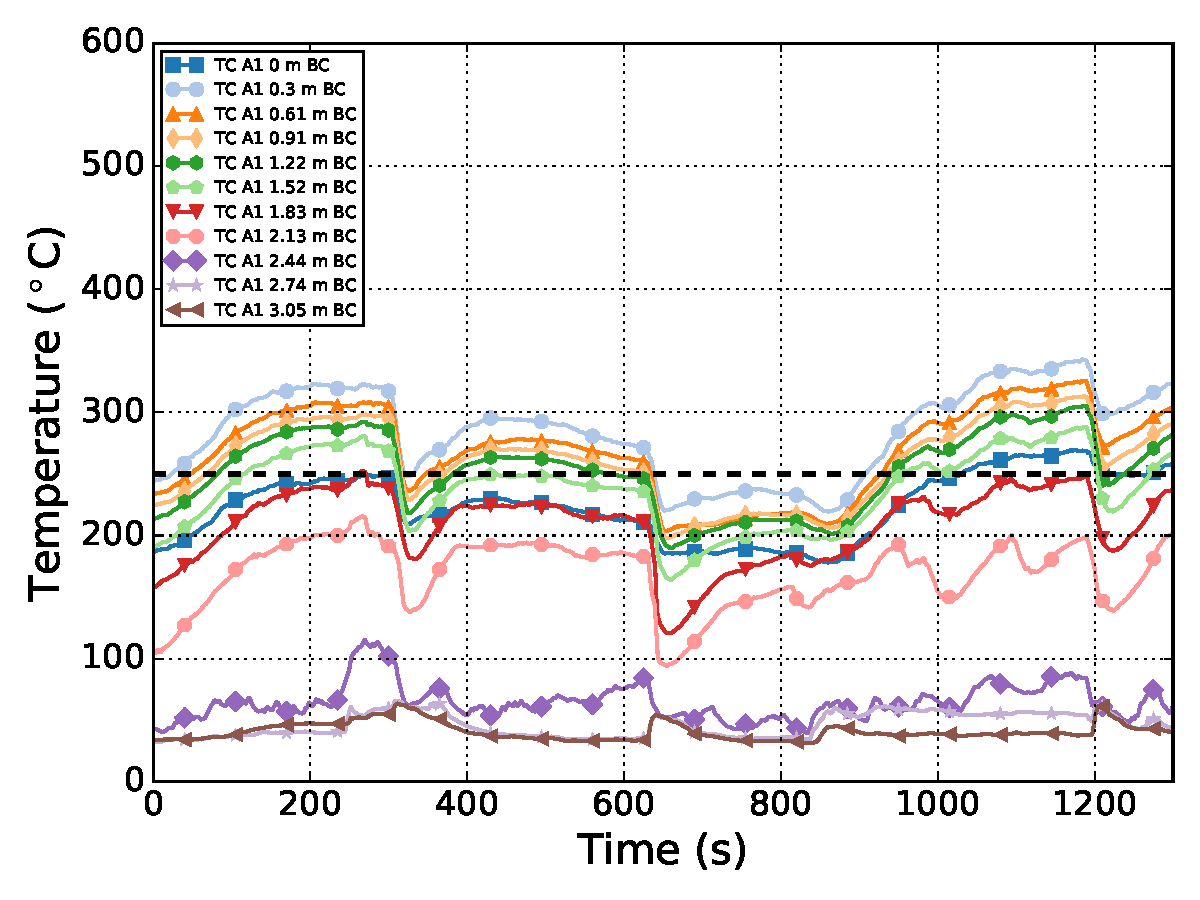
\includegraphics[width=.5\columnwidth]{../Figures/Gas_Cooling/GCSeries12_TC_A1}
	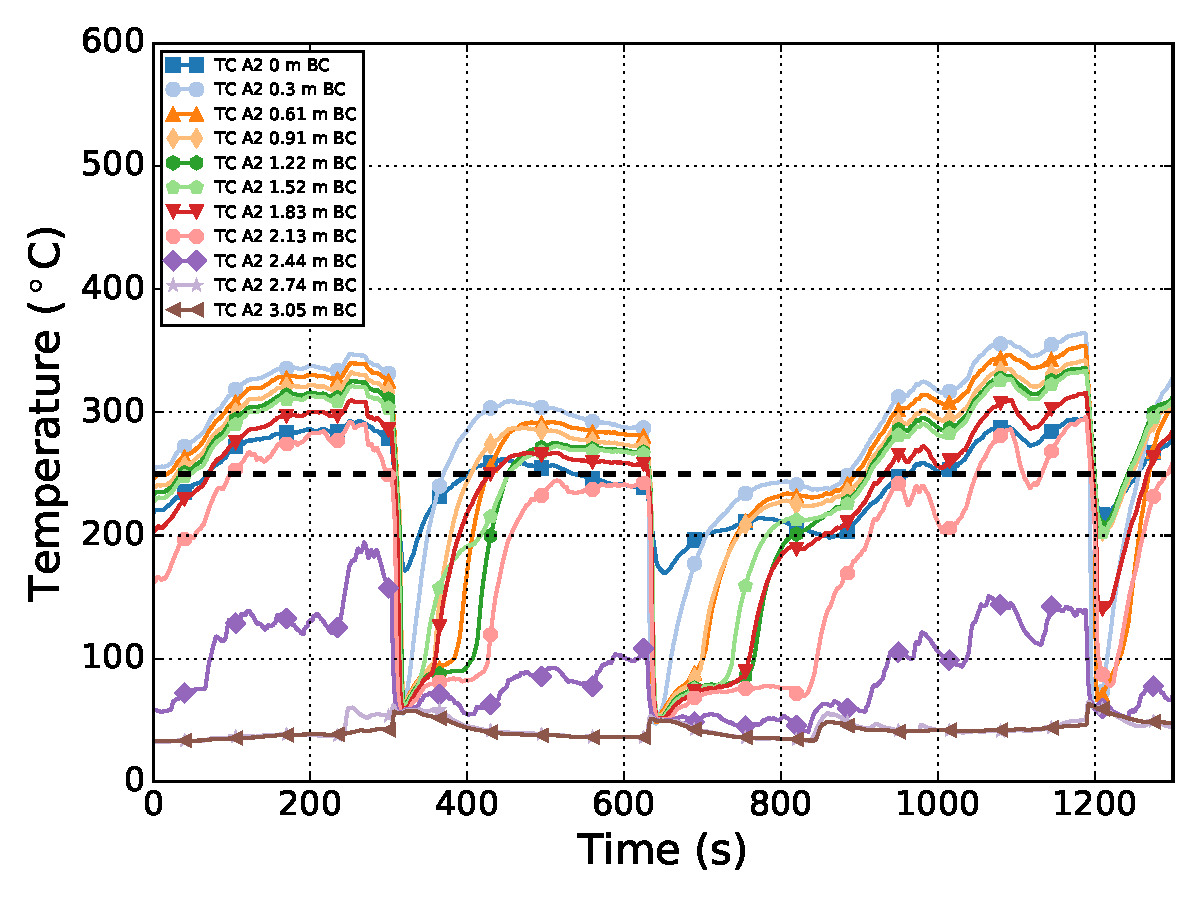
\includegraphics[width=.5\columnwidth]{../Figures/Gas_Cooling/GCSeries12_TC_A2}
	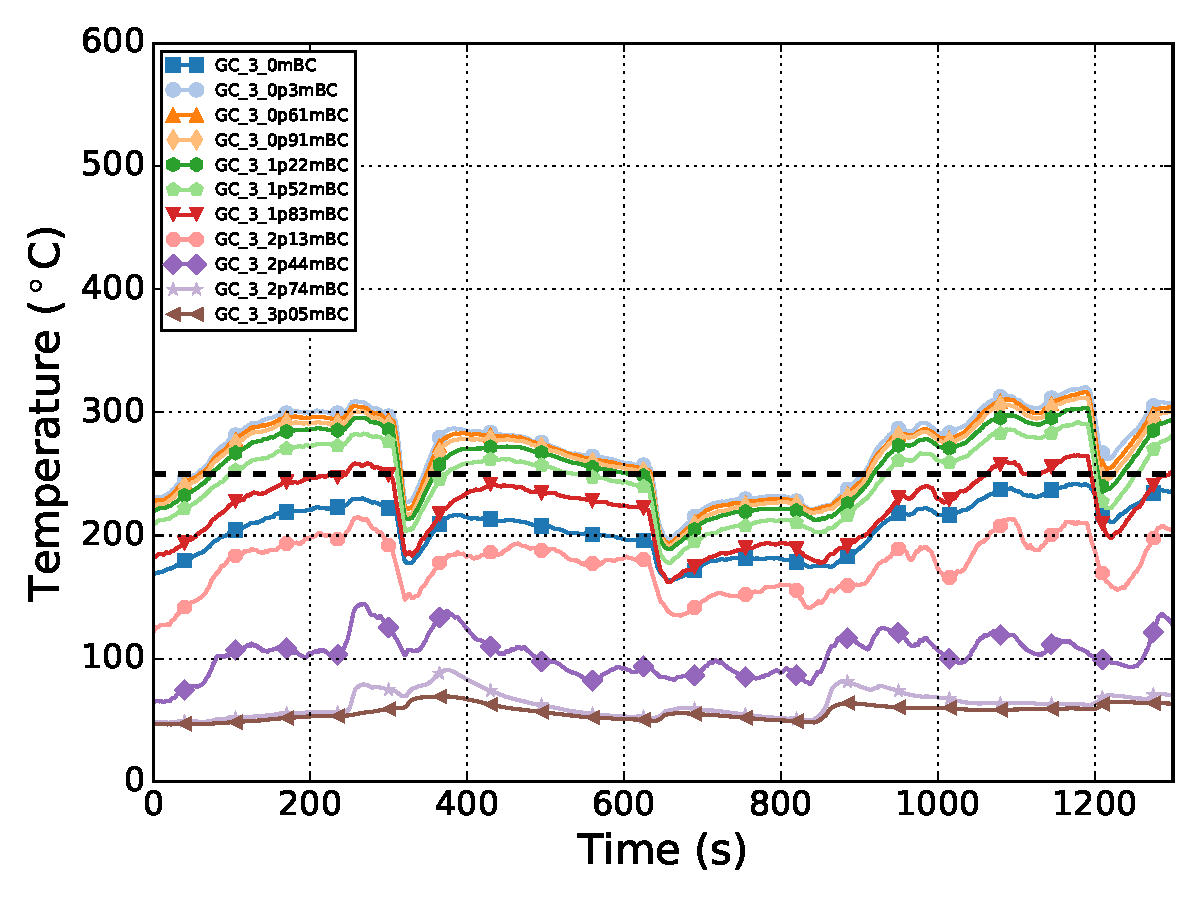
\includegraphics[width=.5\columnwidth]{../Figures/Gas_Cooling/GCSeries12_TC_A3}
	\caption{Time Series of Thermocouple Data from 3 Arrays in Gas Cooling Room with Water as the Suppression Agent}
	\label{fig:gas_cooling_sub1}
\end{figure}

\begin{figure}[ht!]
	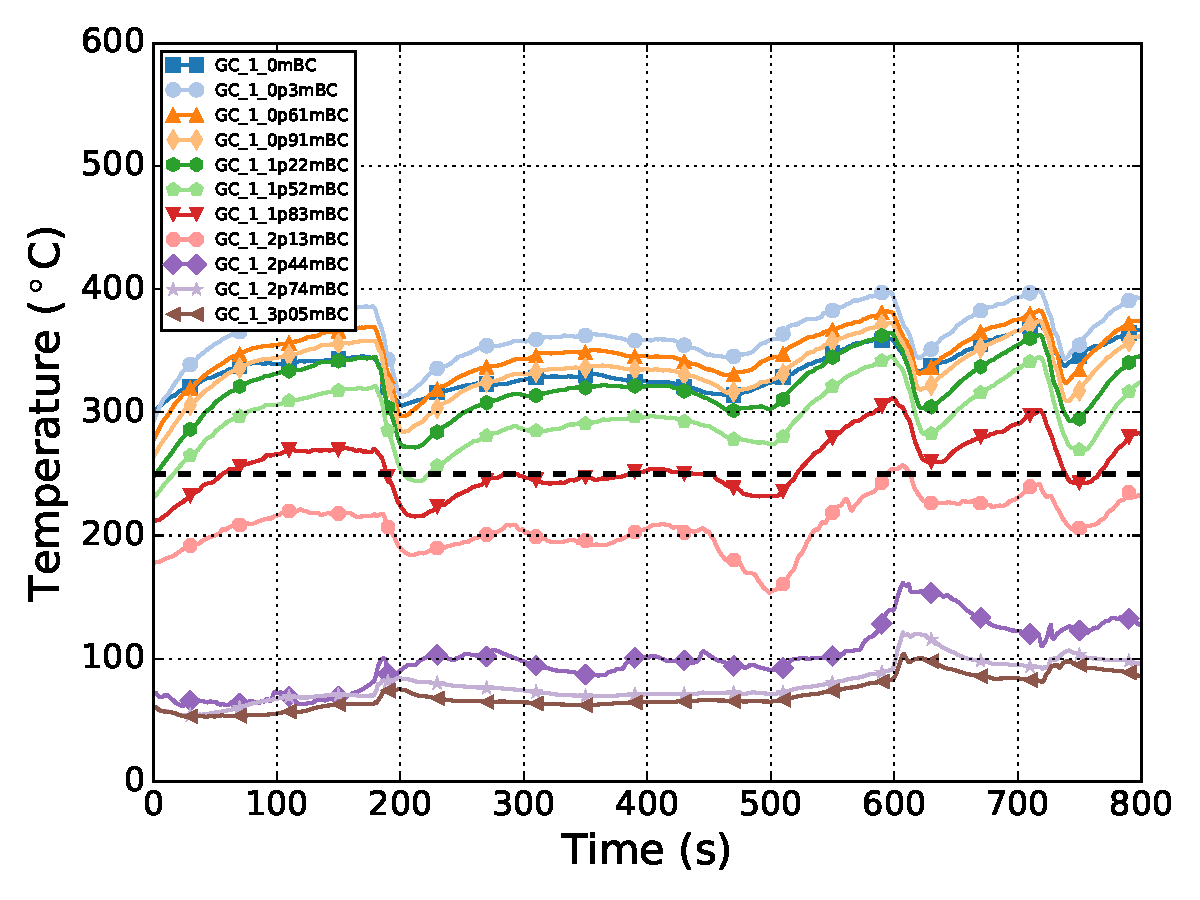
\includegraphics[width=.5\columnwidth]{../Figures/Gas_Cooling/GCSeries52_TC_A1}
	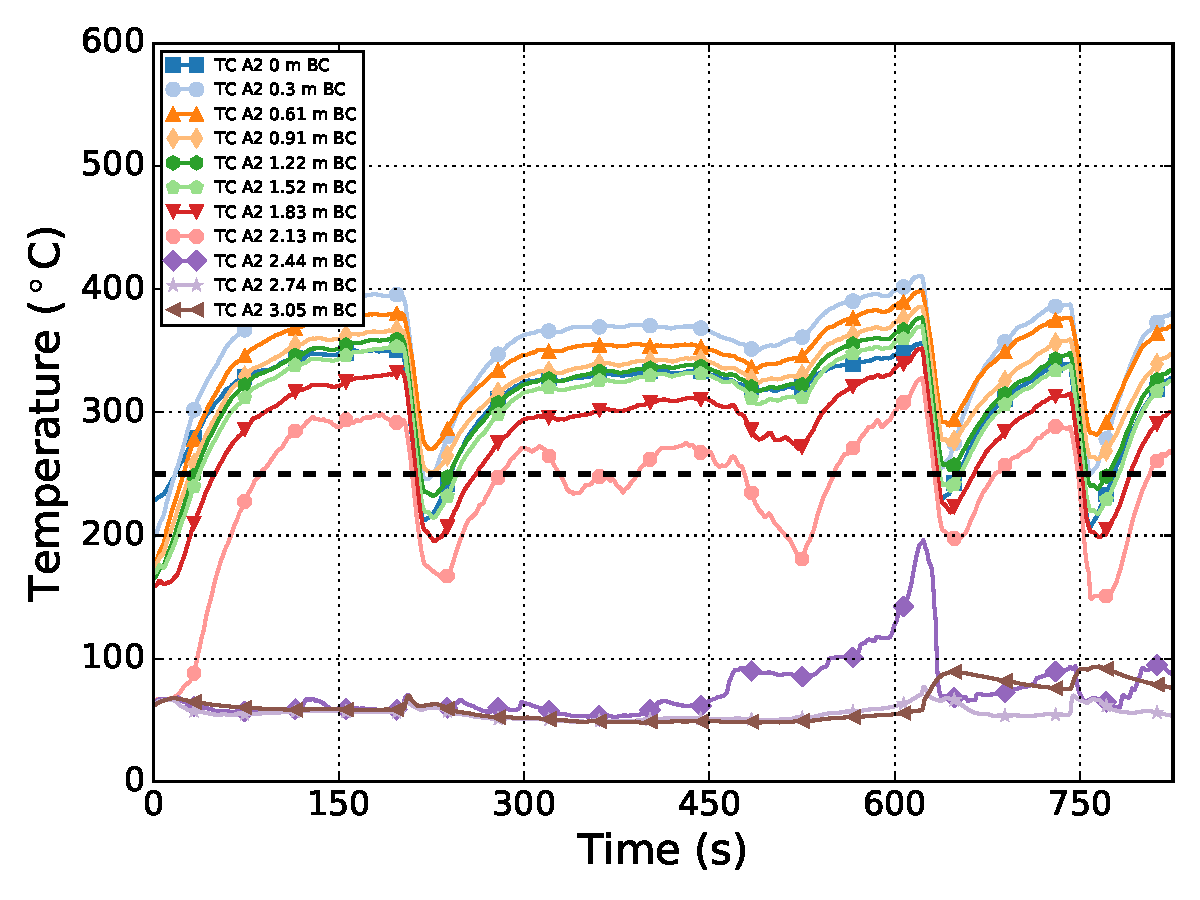
\includegraphics[width=.5\columnwidth]{../Figures/Gas_Cooling/GCSeries52_TC_A2}
	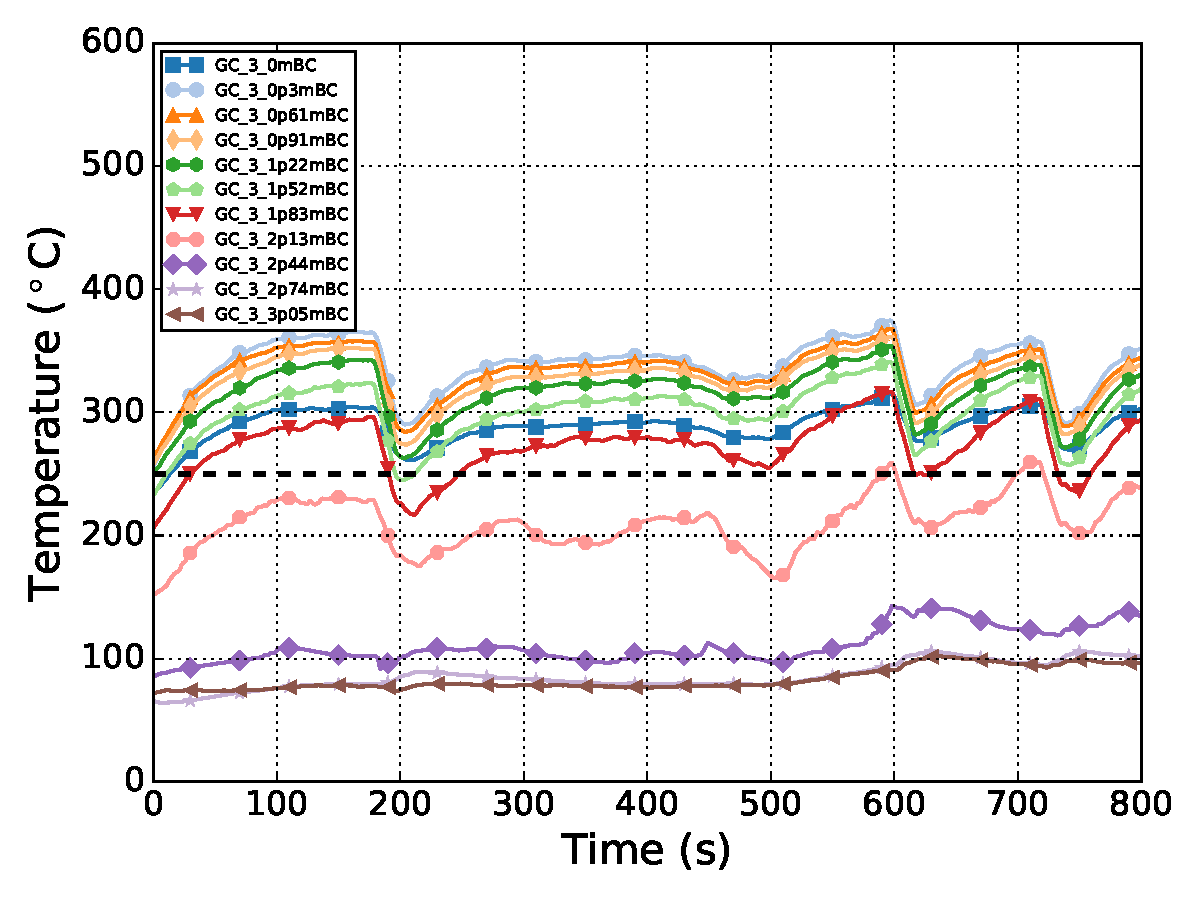
\includegraphics[width=.5\columnwidth]{../Figures/Gas_Cooling/GCSeries52_TC_A3}
	\caption{Time Series of Thermocouple Data from 3 Arrays in Gas Cooling Room with CAF as the Suppression Agent}
	\label{fig:gas_cooling_sub5}
\end{figure}

\clearpage

To better quantify the effectiveness of the suppression agents, the maximum temperature differences associated with each gas cooling event for each agent from the three thermocouple trees were analyzed. Figure~\ref{fig:combined_all} compares the temperature differences at each thermocouple position (via a scatterplot) for 30 of the 88 experiments. The 30 experiments are actually pairs of experiments, 15 water and 15 CAF, that were directly comparable (see Table~\ref{tab:Gas_Cooling_Descriptions}). These experiments included solid streams, straight streams, and narrow fog streams at both nozzle positions. While the total number of experiments was 88, there were a number of experiments that did not have a directly comparable experiment between water and CAF. For example, 12 of the experiments used Class A solution as the suppression agent. Furthermore, gas cooling experiments were conducted with water applied in a wide fog stream, but no experiments with CAF applied in a wide fog stream were conducted because no significant differences were noted between CAF and water in the narrow fog stream experiments. Similarly, larger water flows were examined, but 120 gpm was the maximum water flow that could be generated with the CAFS. So, those experiments are also not included in this comparison. The Mitchell report includes the data for all 88 experiments~\cite{Mitchell:1}. 
   
\begin{table}[!ht]
\centering
\caption{Gas Cooling Comparison Test Descriptions}\label{tab:Gas_Cooling_Descriptions}
\begin{tabular}{clll}
\toprule[1.5pt]
Water Test $\#$  & CAF Test  $\#$	& Stream			  & Position  \\
\midrule
 2               & 6                &  Solid Stream       &  Middle   \\
 3               & 7                &  Solid Stream       &  Middle   \\
 4               & 10               &  Solid Stream       &  Middle   \\
 9               & 11               &  Solid Stream       &  Middle   \\
 17              & 52               &  Solid Stream       &  Middle   \\
 18              & 53               &  Solid Stream       &  Middle   \\
 19              & 54               &  Solid Stream       &  Middle   \\
 16              & 45               &  Straight Stream    &  Middle   \\
 20              & 46               &  Straight Stream    &  Middle   \\
 21              & 47               &  Straight Stream    &  Middle   \\
 22              & 48               &  Straight Stream    &  Middle   \\
 41              & 50               &  Straight Stream    &  Middle   \\
 29              & 12               &  Straight Stream    &  Full Back   \\
 33              & 13               &  Narrow Fog   	  &  Full Back   \\
 34              & 14               &  Narrow Fog   	  &  Full Back   \\
\bottomrule[1.25pt]
\end{tabular}\par
\end{table}

\begin{figure}[!ht]
	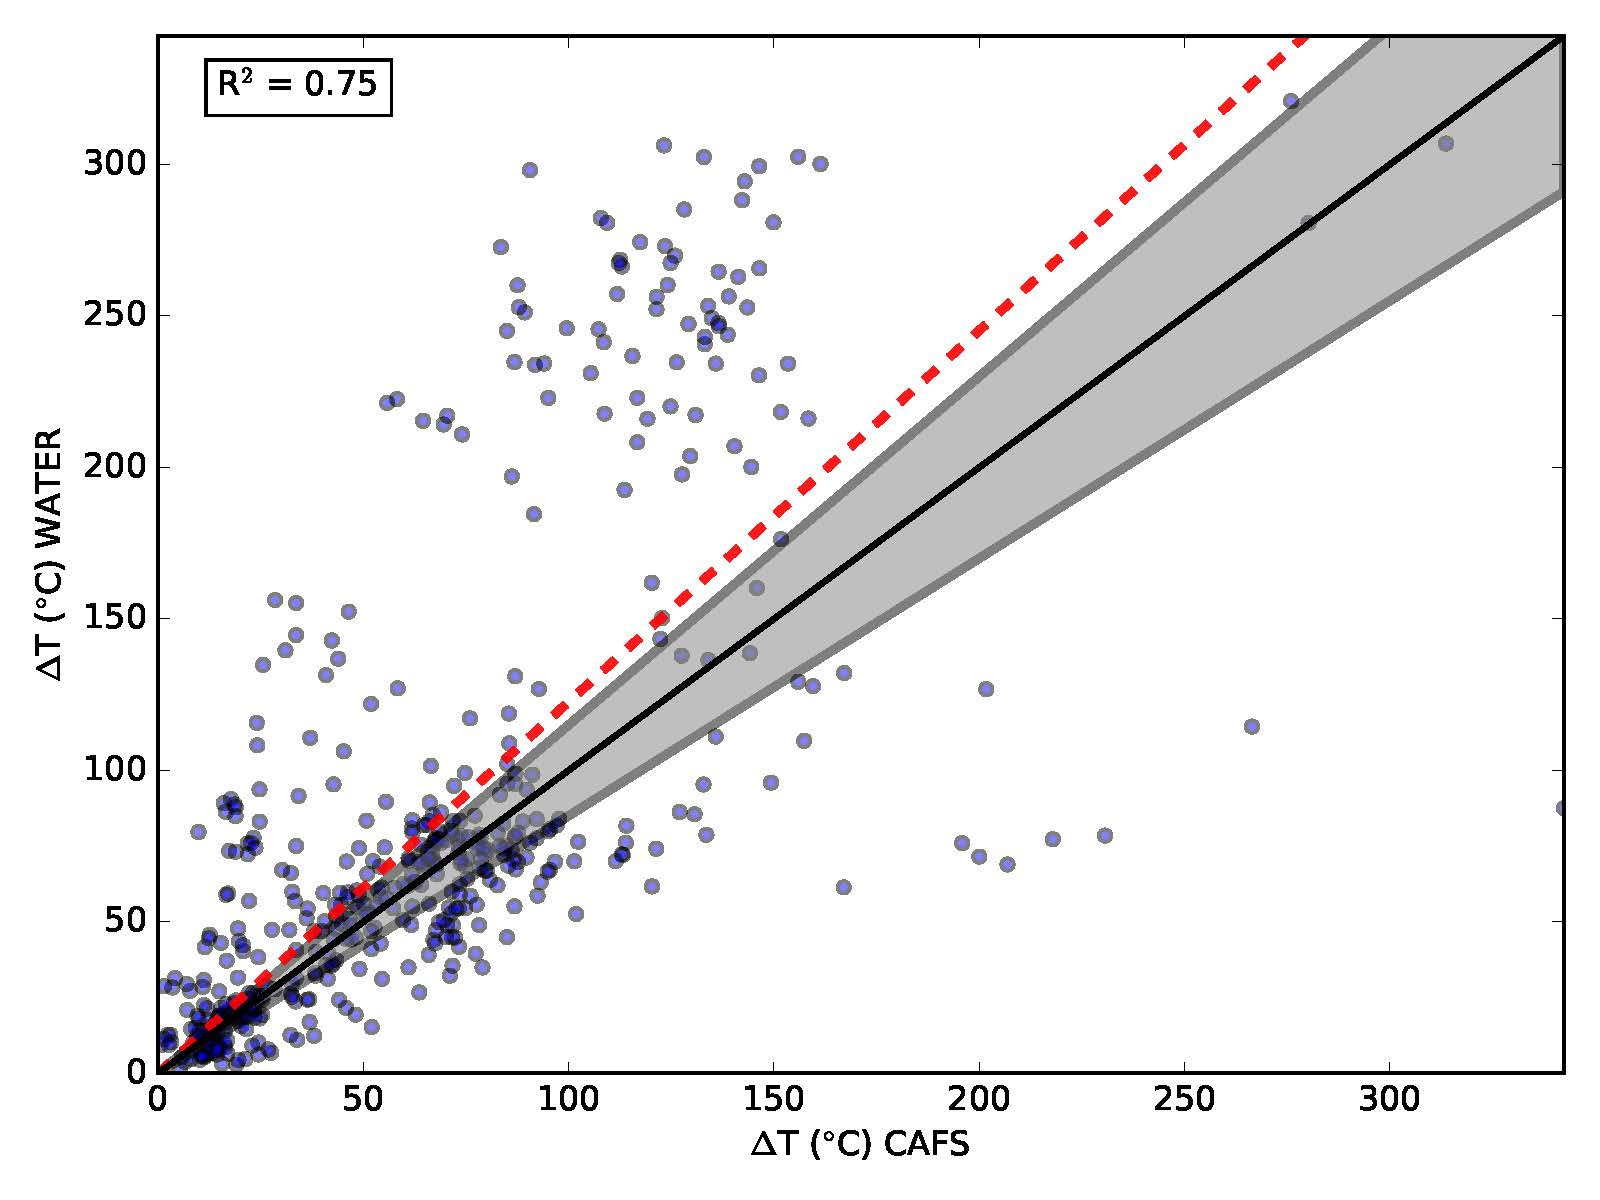
\includegraphics[width=.7\columnwidth]{../Figures/Gas_Cooling/Combined_scatter}
	\caption{CAFS vs Water Gas Cooling Comparison for All Replicate Tests}
	\label{fig:combined_all}
\end{figure}

The circles in Figure~\ref{fig:combined_all} are the maximum temperature differences for each measurement point for all the replicate cooling events. If water and CAF were to have the exact same temperature differences, all the points would fall along the solid black line in the figure. Circles that vary from that line represent measurements where either water (above the line) or CAF (below the line) cooled more significantly than the other agent. The gray area surrounding the solid black line represents measurement uncertainty (Section~\ref{subsec:Uncertainty}). For data that fall within this area, there is an inability to determine which agent was more effective. The red dashed line describes the data by minimizing the differences between the two suppression agents through a linear approximation of the data. Since this line falls above the gray area for the comparison, water shows a better ability to cool gas under the same test criteria as CAF.

The quality of the fit of the red dashed line to the scatter in gas cooling data is represented by the coefficient of determination (R$^2$ in Figure~\ref{fig:combined_all}). The coefficient of determination provides a way to quantify how significant the variation of the data is compared to the least squared error line. Here, the higher the value of R$^2$, the better the ordinary least square line describes the relationship between water and CAF temperature difference comparisons. 

The data can be separated to examine the impact of nozzle position (back or middle position) on the ability to cool gases for each of the suppression agents. Figures~\ref{fig:CAFS_Water_mid} and \ref{fig:CAFS_Water_full} show the cooling comparison for 12 pairs of experiments in the back position and three pairs of experiments in the middle position, respectively.

\begin{figure}[!ht]
	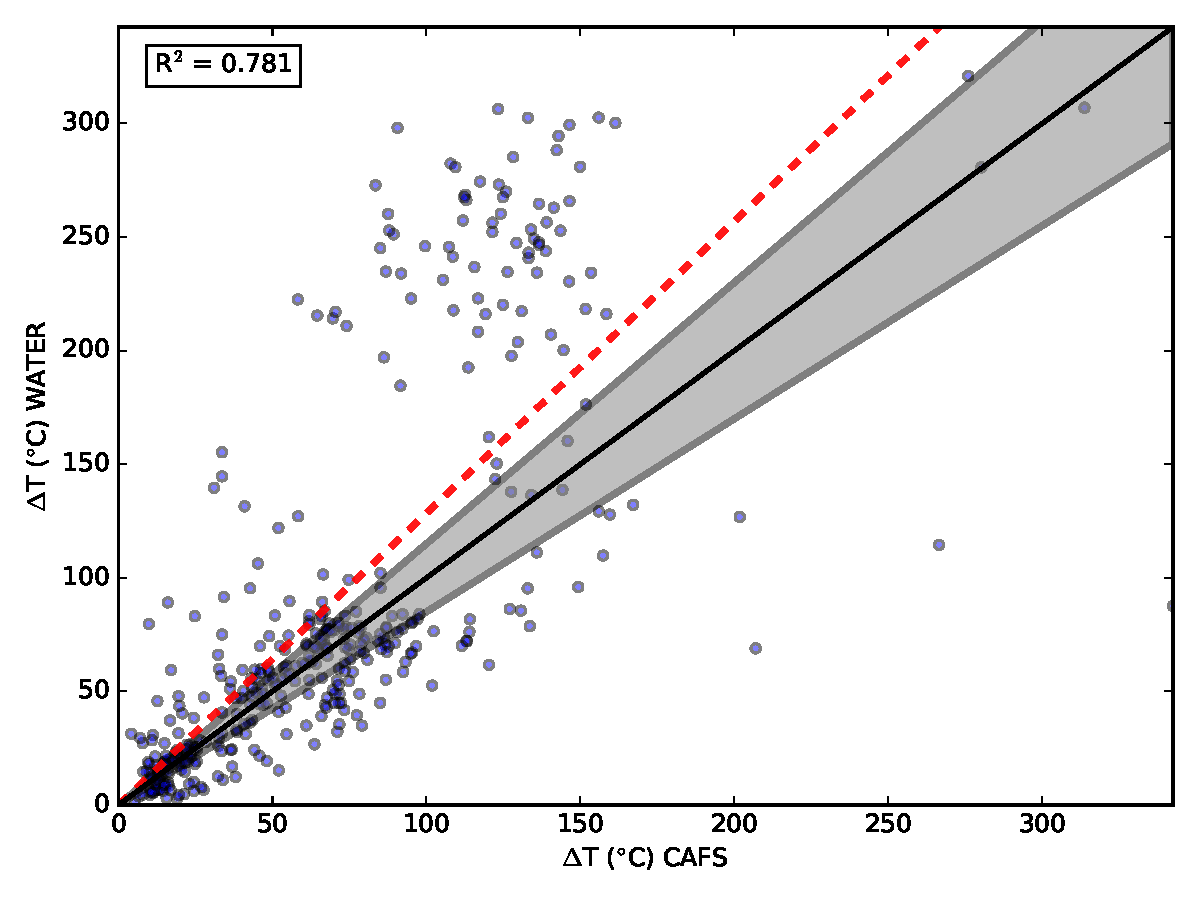
\includegraphics[width=.7\columnwidth]{../Figures/Gas_Cooling/Combined_mid_scatter}
	\caption{CAFS vs Water Gas Cooling Comparison for All Middle Position Replicates}
	\label{fig:CAFS_Water_mid}
\end{figure}

\begin{figure}[!ht]
	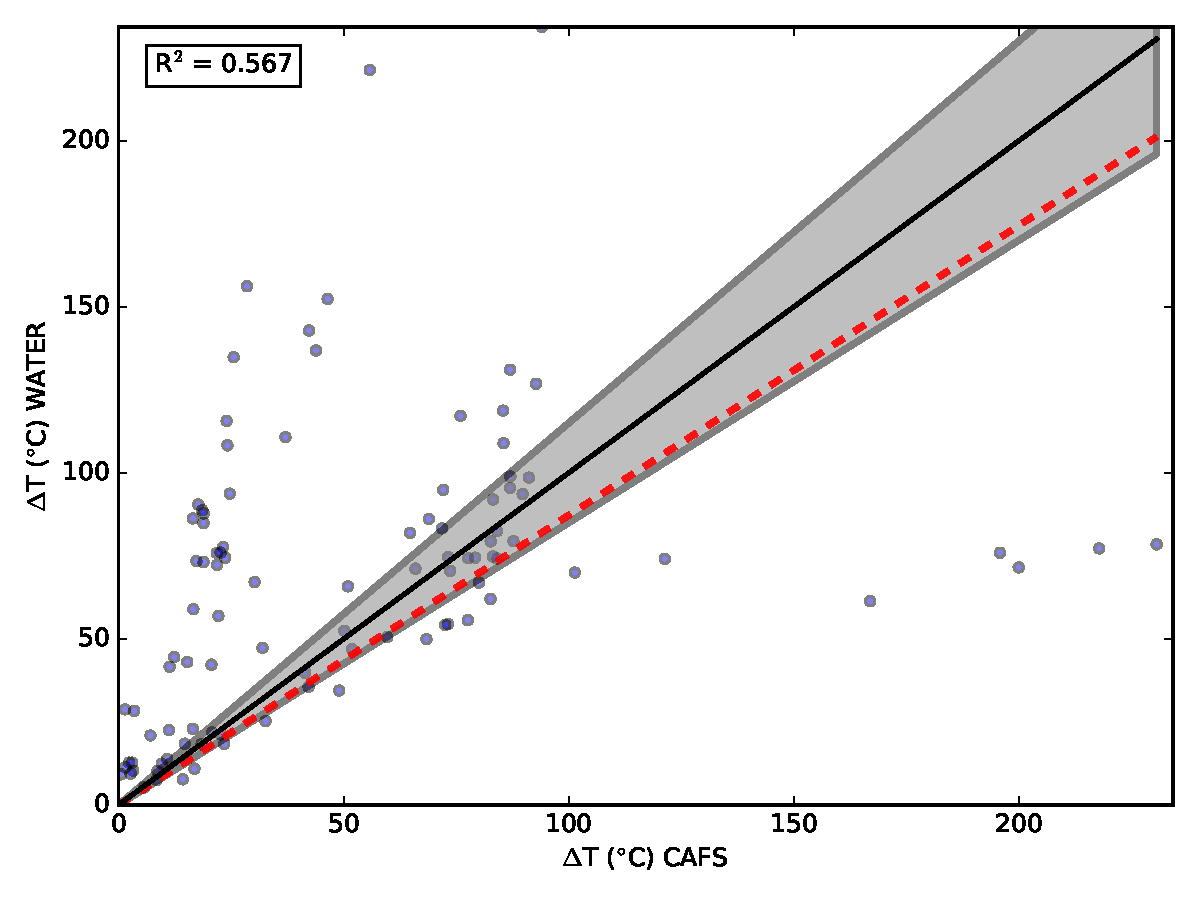
\includegraphics[width=.7\columnwidth]{../Figures/Gas_Cooling/Combined_fullback_scatter}
	\caption{CAFS vs Water Gas Cooling Comparison for All Back Position Replicates}
	\label{fig:CAFS_Water_full}
\end{figure}

For the 12 middle position replicate comparisons (Figure~\ref{fig:CAFS_Water_mid}), the results (via the dashed red line) show that water had a slight advantage in gas cooling relative to CAF. For the three back position replicate comparisons (Figure~\ref{fig:CAFS_Water_full}), the least squared error line falls within the experimental uncertainty. This indicates an inability to distinguish between the two suppression agents with statistical confidence. 

To further analyze the data, the temperature differences can be separated by each of the three thermocouple arrays in the fire room. Figure~\ref{fig:Gas_Cooling_Instrumentation_Dimensions} shows the placement of three thermocouple arrays (TC A1, TC A2, and TC A3). Ideally, the thermocouple is providing an estimate of the temperature of the gas that surrounded it. However, the thermocouple is actually measuring its own temperature. So, if a droplet of water or some CAF clings to a thermocouple, the temperature provided by that thermocouple will be different than the surrounding gas temperature.

Based on the monitor position (see Figure~\ref{fig:Gas_Cooling_Instrumentation_Dimensions}), thermocouple arrays A1 and A2 had more direct impact from the suppression agent compared to thermocouple array A3. As an example, Figure~\ref{fig:Burn_Building_Test_18b} shows the distribution of the agent within the burn building from a spray density test for a straight stream with CAF at the middle position compared to the positions of the thermocouple trees.

\begin{figure}[!ht]
	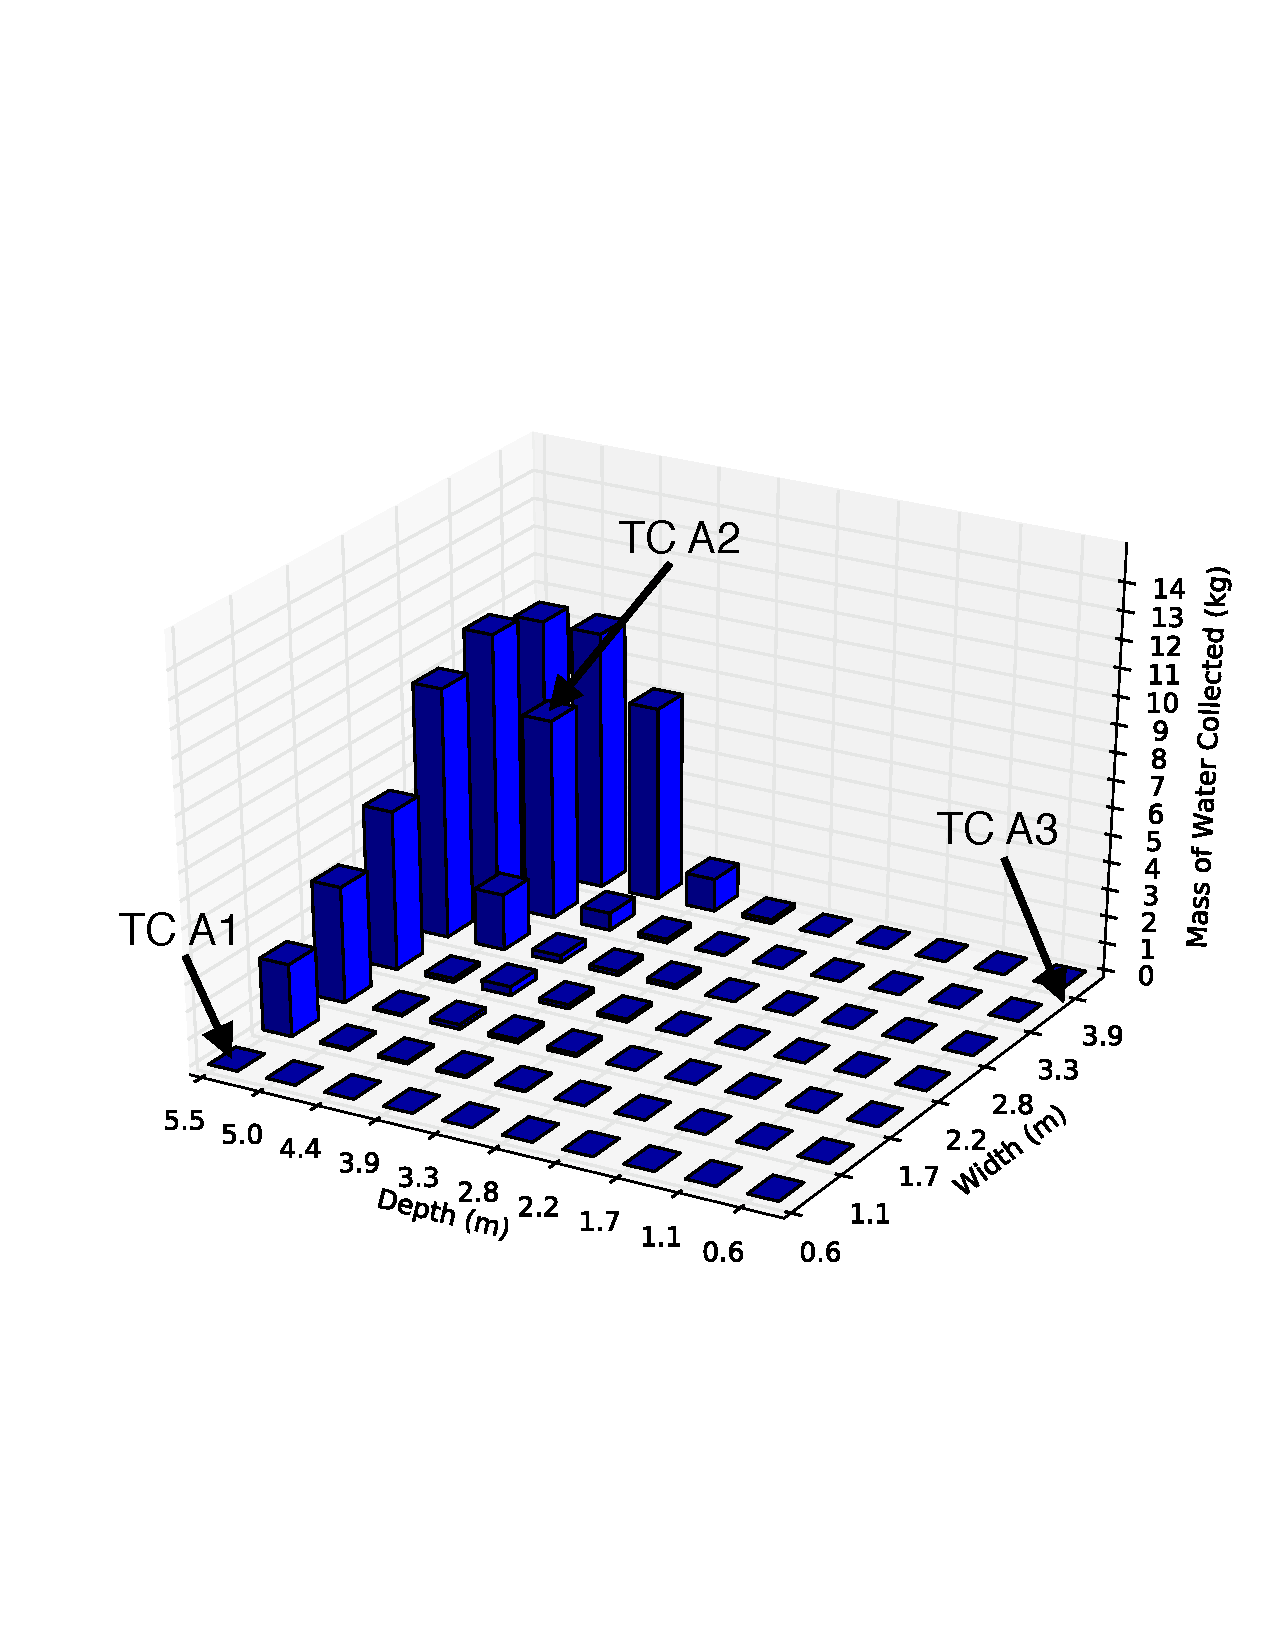
\includegraphics[width=.7\columnwidth]{../Figures/Bars/BB18b}
	\caption{Gas Cooling Spray Density Test 18, CAF, Straight Stream}
	\label{fig:Burn_Building_Test_18b}
\end{figure}

There is a difference in the amount of direct impact from the suppression agent at the three spatial locations. Therefore, the maximum temperature differences for each thermocouple on each of the three arrays should also be analyzed separately. Figures~\ref{fig:CAFS_Water_A1_all}, \ref{fig:CAFS_Water_A2_all}, and \ref{fig:CAFS_Water_A3_all} show the temperature cooling scatter for thermocouple arrays A1, A2, and A3, respectively. Note that thermocouple array A3, the array that had the least amount of direct impact from the suppression agents, has the closest fit compared to the solid black line that represents uniform impact for both suppression agents. The fit lines for A1 and A3 also fall within the experimental uncertainty, meaning that differences in the impact of CAF and water are indistinguishable. Thermocouple array A2, which received the most significant direct impact from the suppression agents, shows a bias towards water being more effective than CAF on cooling the thermocouples. 

\begin{figure}[!ht]
	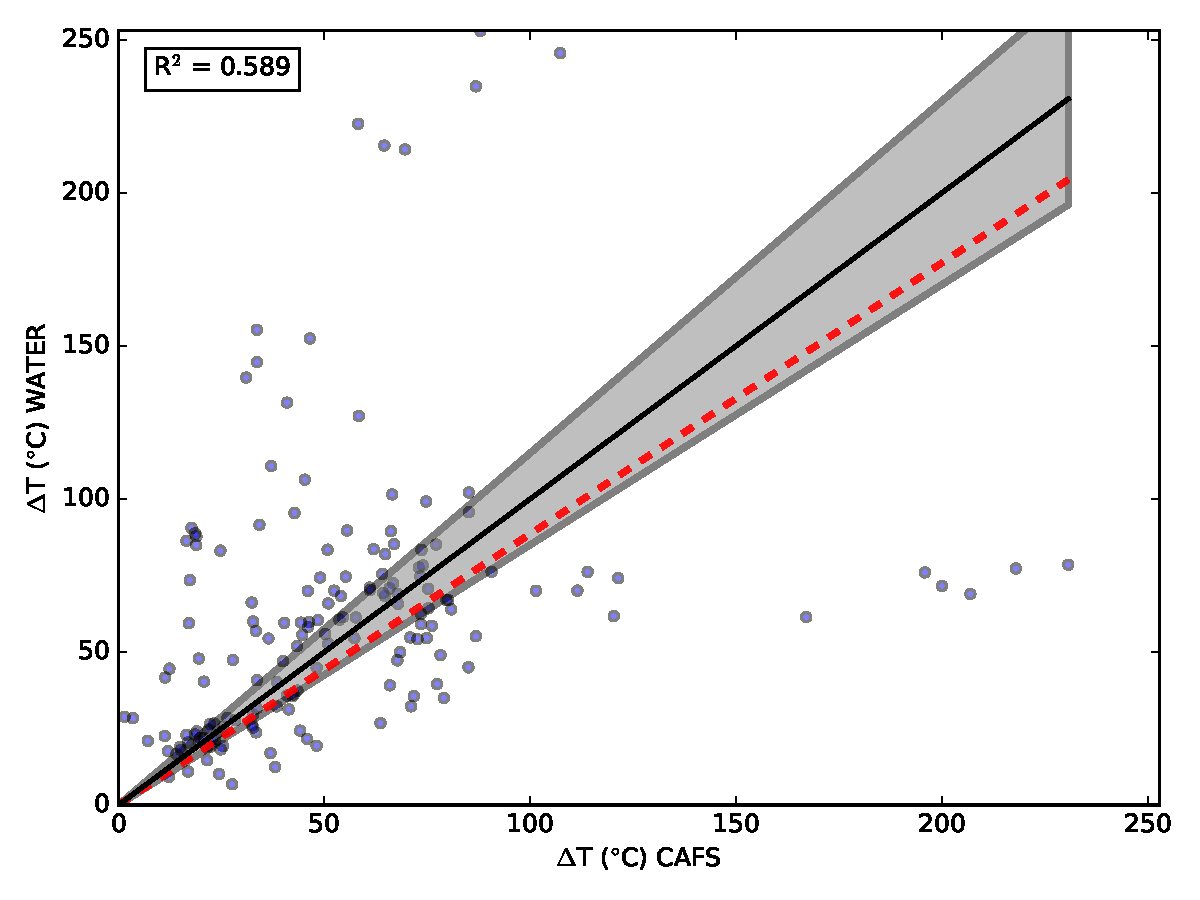
\includegraphics[width=.7\columnwidth]{../Figures/Gas_Cooling/Combined_A1_scatter}
	\caption{CAF vs Water Gas Cooling Comparison for All Thermocouple Tree A1 Experimental Pairs}
	\label{fig:CAFS_Water_A1_all}
\end{figure}

\begin{figure}[!ht]
	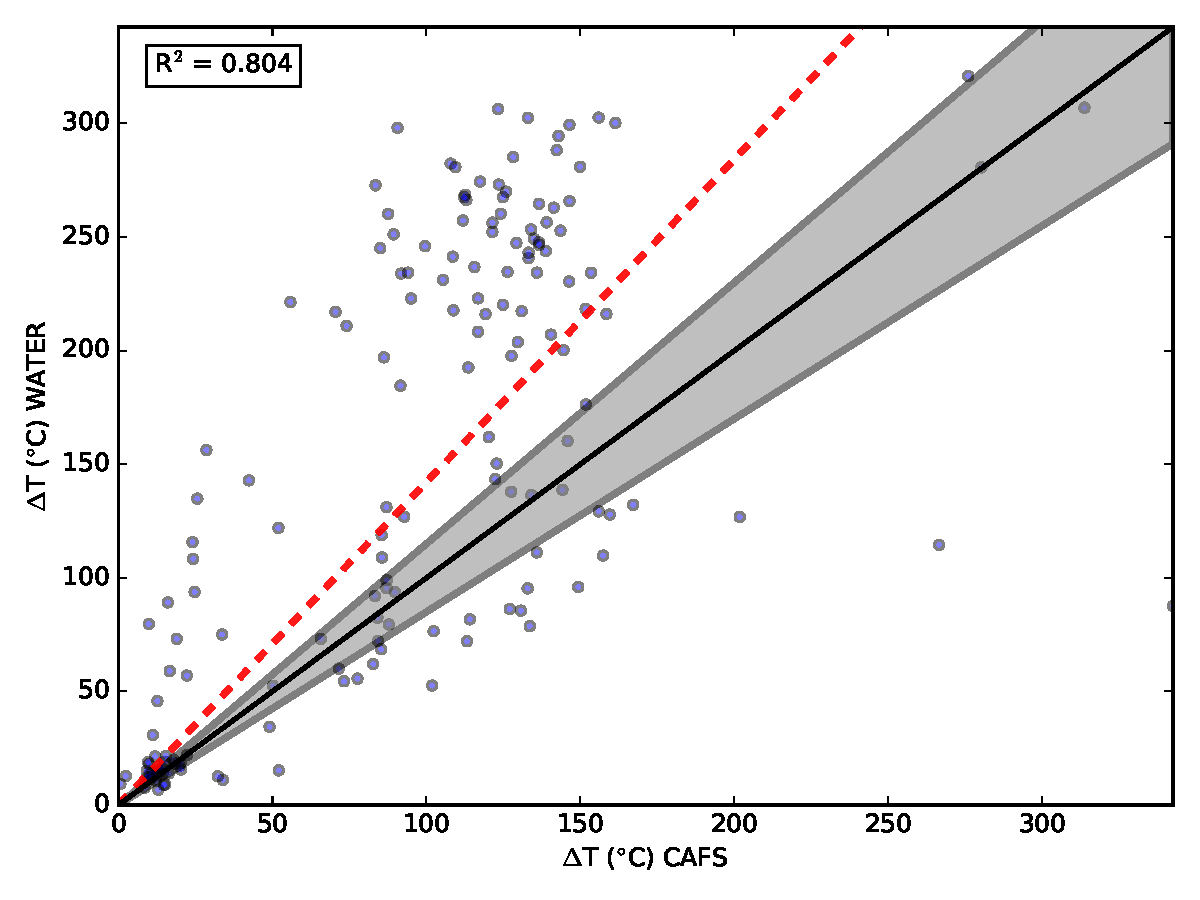
\includegraphics[width=.7\columnwidth]{../Figures/Gas_Cooling/Combined_A2_scatter}
	\caption{CAF vs Water Gas Cooling Comparison for All Thermocouple Tree A2 Experimental Pairs}
	\label{fig:CAFS_Water_A2_all}
\end{figure}

\begin{figure}[!ht]
	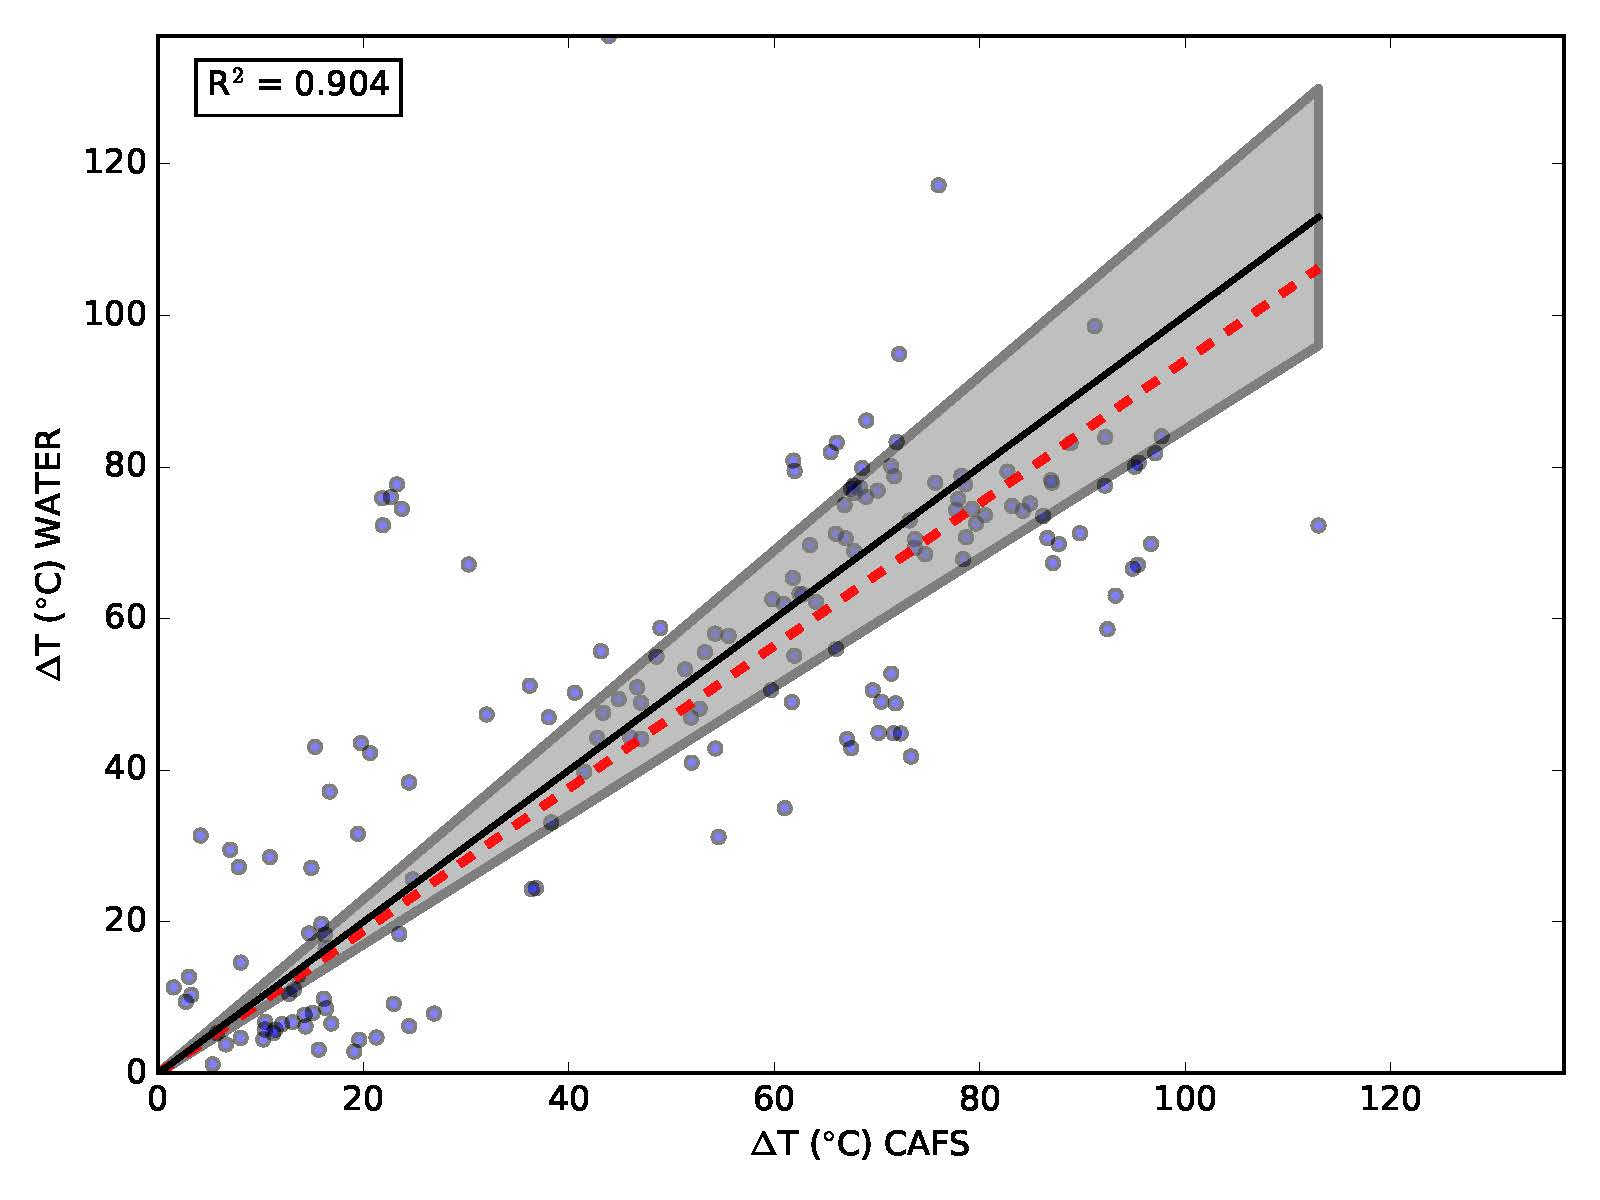
\includegraphics[width=.7\columnwidth]{../Figures/Gas_Cooling/Combined_A3_scatter}
	\caption{CAF vs Water Gas Cooling Comparison for All Thermocouple Tree A3 Experimental Pairs}
	\label{fig:CAFS_Water_A3_all}
\end{figure}

\clearpage

The thermocouple array data can also be decomposed as a function of nozzle position: 12 middle position experimental pairs and three back experimental pairs. Figures~\ref{fig:CAFS_Water_A1_mid}, \ref{fig:CAFS_Water_A2_mid}, and \ref{fig:CAFS_Water_A3_mid} show the temperature difference scatter at thermocouple arrays A1, A2, and A3 respectively for the 12 replicate tests with the monitor nozzle in the middle position. Figures~\ref{fig:CAFS_Water_A1_back}, \ref{fig:CAFS_Water_A2_back}, and \ref{fig:CAFS_Water_A3_back} show the temperature difference scatter at thermocouple arrays A1, A2, and A3 respectively for the three replicate tests with the monitor nozzle in the back position. Again, note that the best fit occurs with the data from thermocouple array 3 for both nozzle positions. This analysis of the data results in the same conclusions as the analysis from the Mitchell paper \cite{Mitchell:1}: the gas cooling performance of CAF is similar to water under these conditions. Or, more accurately, water is nearly always equal to or better than CAF.

\begin{figure}[!ht]
	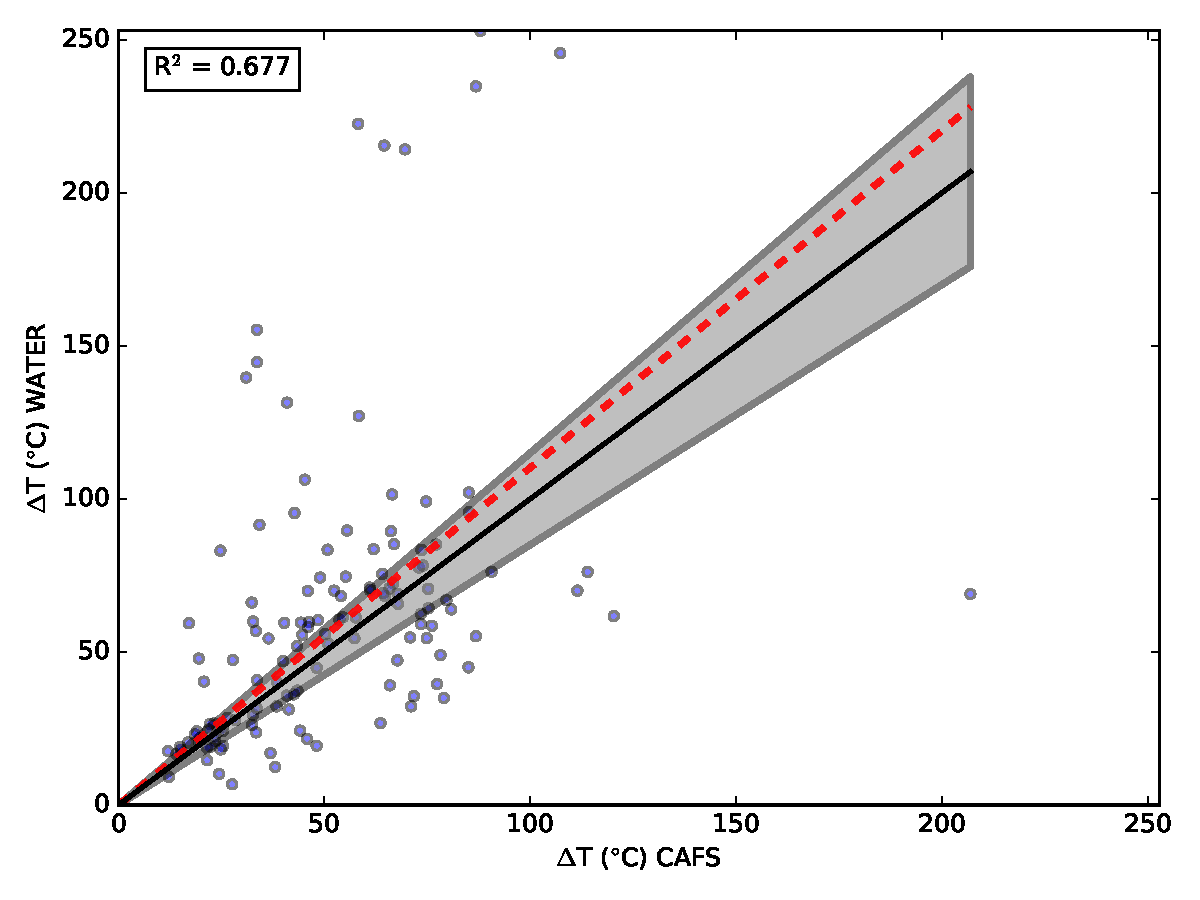
\includegraphics[width=.7\columnwidth]{../Figures/Gas_Cooling/Combined_mid_A1_scatter}
	\caption{CAF vs Water Gas Cooling Comparison for Middle Position Thermocouple Tree A1 Replicates}
	\label{fig:CAFS_Water_A1_mid}
\end{figure}

\begin{figure}[!ht]
	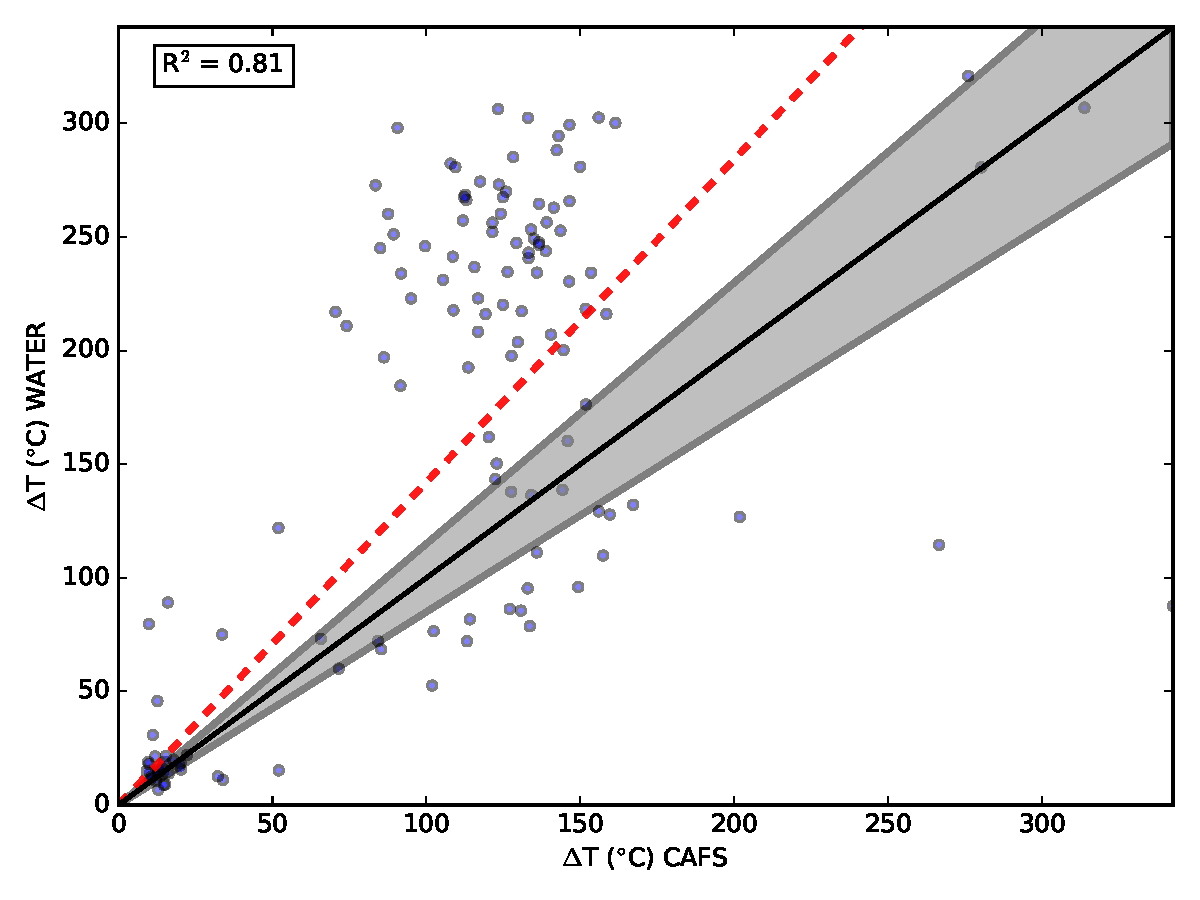
\includegraphics[width=.7\columnwidth]{../Figures/Gas_Cooling/Combined_mid_A2_scatter}
	\caption{CAF vs Water Gas Cooling Comparison for Middle Position Thermocouple Tree A2 Replicates}
	\label{fig:CAFS_Water_A2_mid}
\end{figure}

\begin{figure}[!ht]
	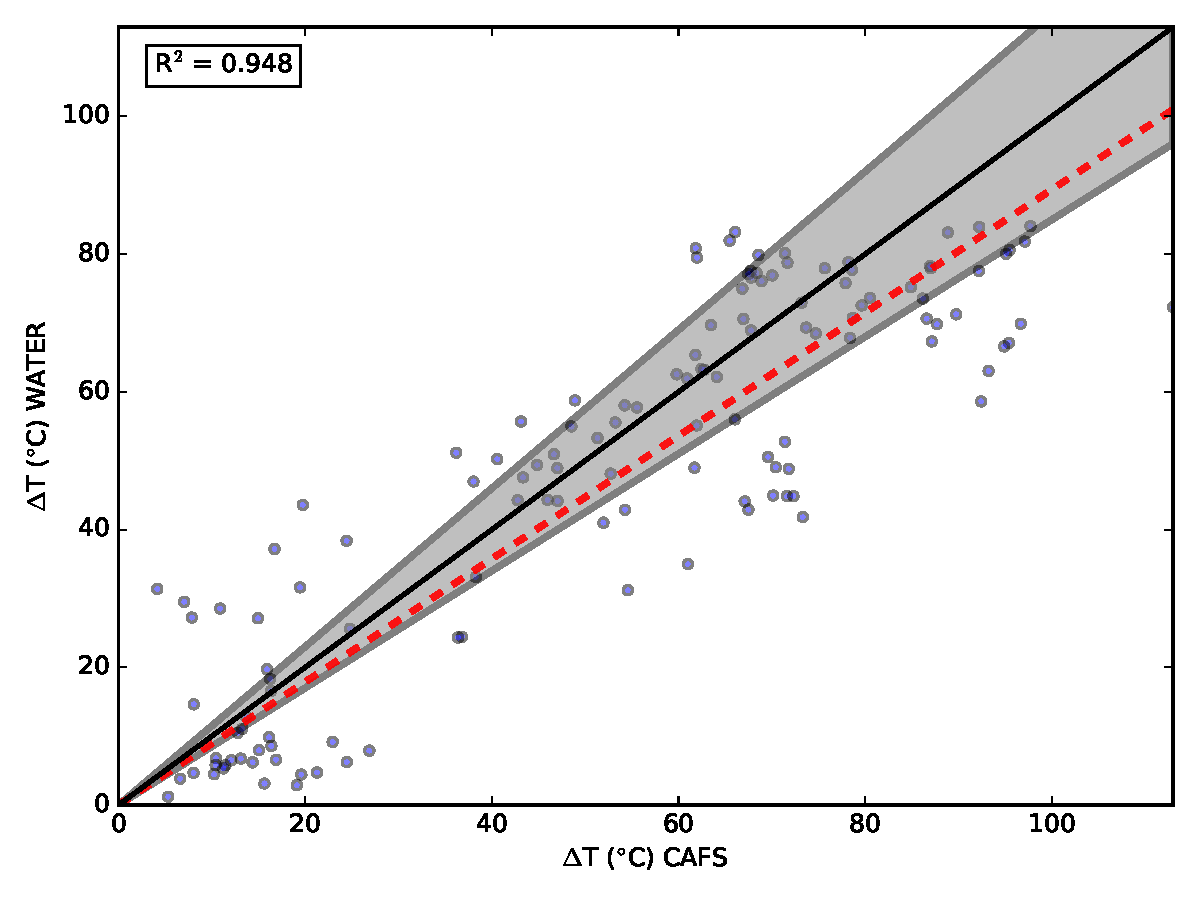
\includegraphics[width=.7\columnwidth]{../Figures/Gas_Cooling/Combined_mid_A3_scatter}
	\caption{CAF vs Water Gas Cooling Comparison for Middle Position Thermocouple Tree A3 Replicates}
	\label{fig:CAFS_Water_A3_mid}
\end{figure}

\begin{figure}[!ht]
	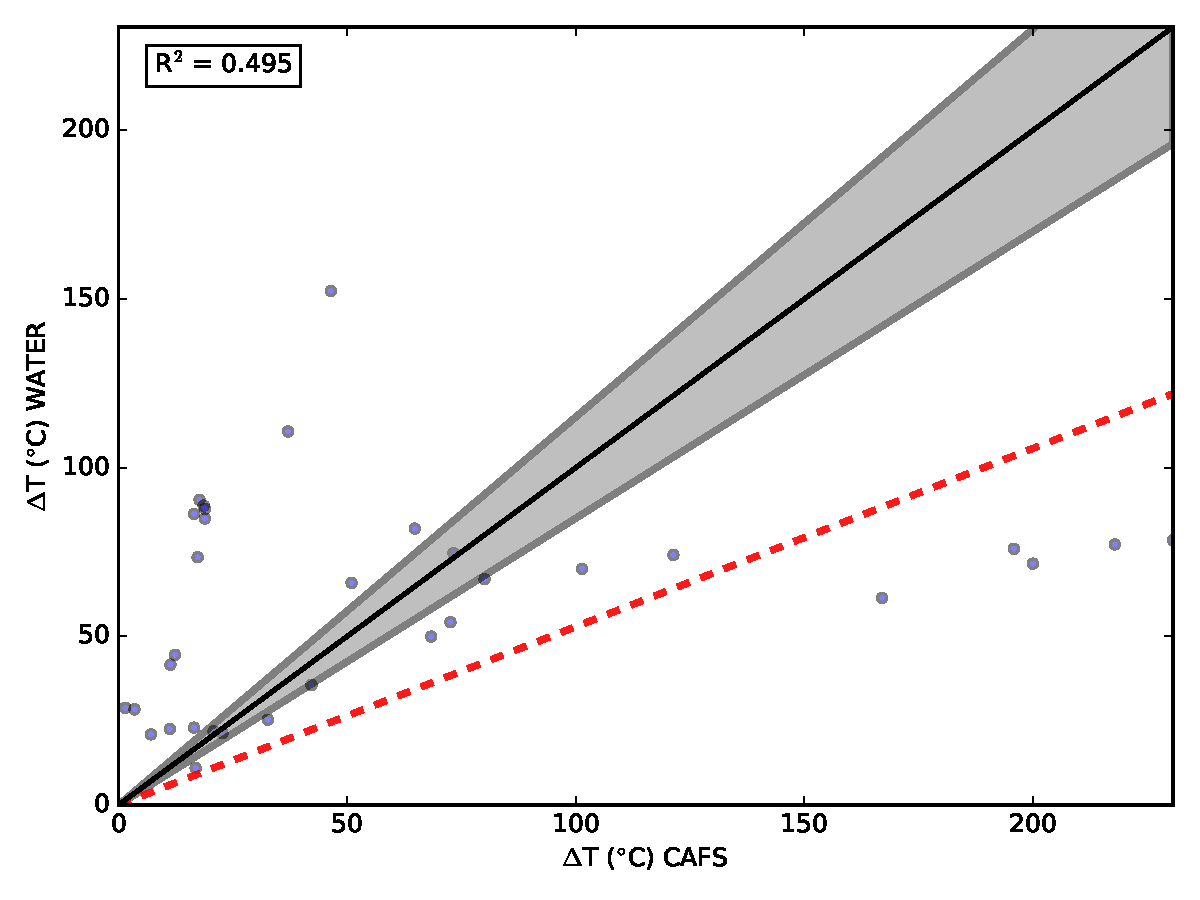
\includegraphics[width=.7\columnwidth]{../Figures/Gas_Cooling/Combined_fullback_A1_scatter}
	\caption{CAF vs Water Gas Cooling Comparison for Back Position Thermocouple Tree A1 Replicates}
	\label{fig:CAFS_Water_A1_back}
\end{figure}

\begin{figure}[!ht]
	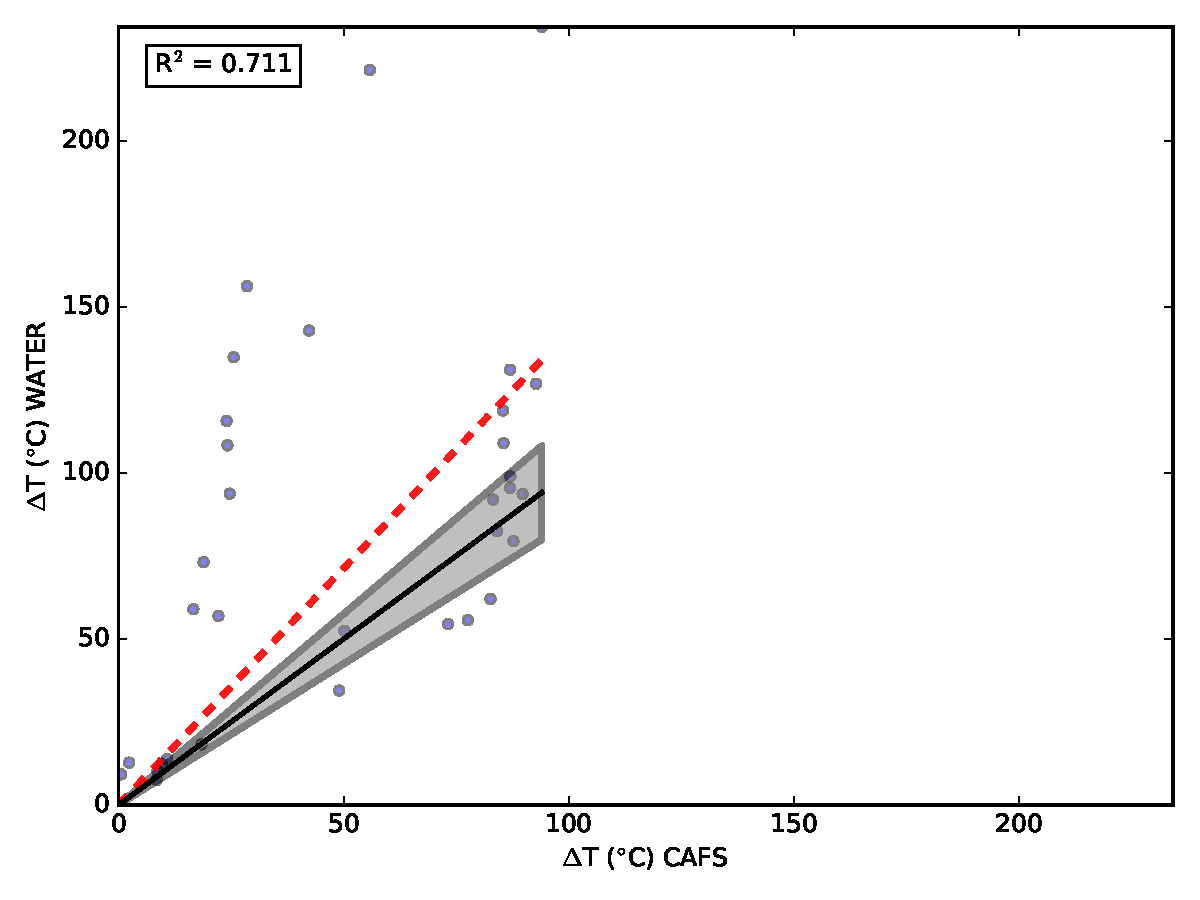
\includegraphics[width=.7\columnwidth]{../Figures/Gas_Cooling/Combined_fullback_A2_scatter}
	\caption{CAF vs Water Gas Cooling Comparison for Back Position Thermocouple Tree A2 Replicates}
	\label{fig:CAFS_Water_A2_back}
\end{figure}

\begin{figure}[!ht]
	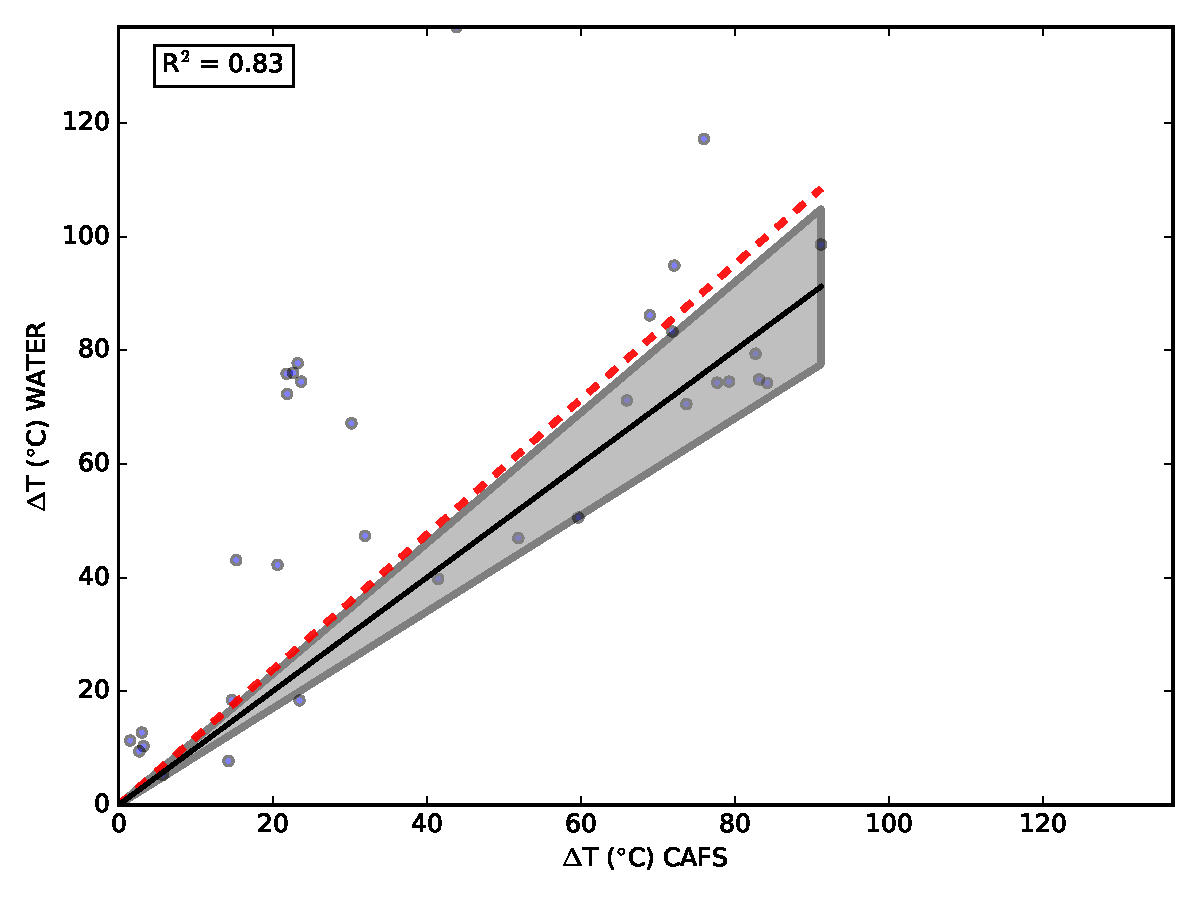
\includegraphics[width=.7\columnwidth]{../Figures/Gas_Cooling/Combined_fullback_A3_scatter}
	\caption{CAF vs Water Gas Cooling Comparison for Back Position Thermocouple Tree A3 Replicates}
	\label{fig:CAFS_Water_A3_back}
\end{figure}


\clearpage

\section{Fire Suppression}
\label{sec:Fire_Suppression}

\subsubsection*{Single-Story Structure}
\label{sec:fire_supp_single}

There were 12 suppression tests conducted in the single-story, purpose-built concrete structure. Eight of the experiments used a fuel load comprised of typical household furnishings that included wooden wall paneling, two sofas, two overstuffed chairs, carpet, and padding (Section~\ref{sec:fire_suppression_furniture_fuel}). The other four experiments used a wood pallet fuel load in a space with the ceiling and walls composed of wood-based materials (Section~\ref{sec:fire_suppression_pallet_fuel}). Ignition occurred in the rear of the single-story structure, and the available ventilation was through the front doorway. For eight of the experiments, a rear window was opened to provide additional ventilation (see Table~\ref{tab:Test_Descriptions}). The fires were intended to replicate post-flashover residential room and contents fires. Hose lines were pre-deployed with fixed nozzles set in two locations: one in the hallway on the approach to the burn room (hallway nozzle) and one just inside the burn room to the right side of the hallway (door nozzle). Each nozzle flowed 15~s of water or CAF depending on the test. The hallway nozzle was intended to simulate a crew advancing into a structure towards the burn room. Suppression from this location would be in the form of gas cooling, as the stream was not aimed at the seat of the fire (indirect interior attack).  After the hallway nozzle was shutdown, there was a 15~s time period of no nozzle flow to simulate the crew advancing into the doorway of the fire room. The door nozzle was positioned just to the side of the entry door.  It was also opened and flowed for approximately 15~s. The door nozzle was aimed in the direction of the seat of the fire (direct interior attack). Table~\ref{tab:Test_Descriptions} provides an overview of the suppression tests conducted.

\begin{table}[!ht]
\centering
\caption{Single-Story Fire Suppression Test Descriptions}\label{tab:Test_Descriptions}
\begin{tabular}{clllll}
\toprule[1.5pt]
Test $\#$  & Name	& Stream			& Flow Rate		& Fuel           & Ventilation     \\
\midrule
 1 & CAF~1    &  Narrow Fog   &  120~gpm/60~cfm   & Furniture      & Door            \\
 2 & Water~1  &  Narrow Fog  	&  120~gpm    		& Furniture      & Door            \\
 3 & CAF~2    &  Solid Stream       &  120~gpm/60~cfm   & Furniture      & Door            \\
 4 & Water~2  &  Solid Stream       &  120~gpm    		& Furniture      & Door            \\
 5 & Water~3  &  Narrow Fog  	&  120~gpm    		& Furniture      & Door + Window   \\
 6 & CAF~3    &  Narrow Fog   &  120~gpm/60~cfm   & Furniture      & Door + Window   \\
 7 & Water~4  &  Narrow Fog  	&  120~gpm    		& Furniture      & Door + Window   \\
 8 & CAF~4    &  Narrow Fog   &  120~gpm/60~cfm   & Furniture      & Door + Window   \\
 9 & Water~5  &  Narrow Fog  	&  120~gpm   		& Wood           & Door + Window   \\
10 & CAF~5    &  Narrow Fog   &  120~gpm/60~cfm   & Wood           & Door + Window   \\
11 & Water~6  &  Narrow Fog  	&  120~gpm    		& Wood           & Door + Window   \\
12 & CAF~6    &  Narrow Fog   &  120~gpm/60~cfm   & Wood           & Door + Window   \\
\bottomrule[1.25pt]
\end{tabular}\par
\end{table}

Table~\ref{tab:Test_Results} provides the impact of the two nozzle applications for the water and CAF tests. The table lists the change in temperature 0.3~m (1~ft) below the ceiling and 0.3~m (1~ft) above the floor as well as the change in heat flux 0.15~m (6~in) above the floor at the measurement location closest to the fire. These values reported in the table are immediately before and after the 15~s application period to assess the application agent, stream, and location on interior conditions. Recall that there was a 15~s gap between the hallway nozzle flow and the door nozzle flow. The amount of temperature change during the period in between nozzle flows is shown by comparing the temperature at the end of the hallway nozzle flow period with the temperature at the beginning of the door nozzle flow period.

\begin{table}[!ht]
\centering
\caption{Single-Story Fire Suppression Results}\label{tab:Test_Results}
\begin{tabular}{lccc}
\toprule[1.5pt]
                 & \multicolumn{2}{c}{Temperature Change}                                    & Heat Flux Change \\
Test \# \& Nozzle	         & 0.3~m Below Ceiling                 & 0.3~m  Above Floor	                 & 0.15~m Above Floor \\
\midrule
CAF~1 Hallway    & 690~$^{\circ}$C - 180~$^{\circ}$C   & 590~$^{\circ}$C - 150~$^{\circ}$C   & 70~kW/m$^2$ - 20~kW/m$^2$  \\
CAF~1 Door       & 170~$^{\circ}$C - 80~$^{\circ}$C    & 80~$^{\circ}$C - 60~$^{\circ}$C     & 25~kW/m$^2$ - 0~kW/m$^2$  \\ [.25cm]
Water~1 Hallway  & 720~$^{\circ}$C - 220~$^{\circ}$C   & 700~$^{\circ}$C - 120~$^{\circ}$C   & 40~kW/m$^2$ - 15~kW/m$^2$  \\
Water~1 Door     & 120~$^{\circ}$C - 80~$^{\circ}$C    & 80~$^{\circ}$C - 70~$^{\circ}$C     & 25~kW/m$^2$ - 0~kW/m$^2$  \\ [.25cm]
CAF~2 Hallway    & 590~$^{\circ}$C - 290~$^{\circ}$C   & 500~$^{\circ}$C - 110~$^{\circ}$C   & 65~kW/m$^2$ - 10~kW/m$^2$  \\
CAF~2 Door       & 80~$^{\circ}$C -  70~$^{\circ}$C    & 70~$^{\circ}$C - 50~$^{\circ}$C     & 30~kW/m$^2$ - 5~kW/m$^2$  \\ [.25cm]
Water~2 Hallway  & 640~$^{\circ}$C - 410~$^{\circ}$C   & 500~$^{\circ}$C - 230~$^{\circ}$C   & 70~kW/m$^2$ - 20~kW/m$^2$  \\
Water~2 Door     & 460~$^{\circ}$C - 300~$^{\circ}$C   & 200~$^{\circ}$C - 140~$^{\circ}$C   & 20~kW/m$^2$ - 5~kW/m$^2$  \\ [.25cm]
Water~3 Hallway  & 610~$^{\circ}$C - 300~$^{\circ}$C   & 580~$^{\circ}$C - 170~$^{\circ}$C   & 60~kW/m$^2$ - 10~kW/m$^2$  \\
Water~3 Door     & 210~$^{\circ}$C - 130~$^{\circ}$C   & 60~$^{\circ}$C - 40~$^{\circ}$C     & 30~kW/m$^2$ - 5~kW/m$^2$  \\ [.25cm]
CAF~3 Hallway    & 880~$^{\circ}$C - 300~$^{\circ}$C   & 780~$^{\circ}$C - 230~$^{\circ}$C   & 80~kW/m$^2$ - 10~kW/m$^2$  \\
CAF~3 Door       & 190~$^{\circ}$C - 60~$^{\circ}$C    & 80~$^{\circ}$C - 60~$^{\circ}$C     & 15~kW/m$^2$ - 5~kW/m$^2$  \\ [.25cm]
Water~4 Hallway  & 850~$^{\circ}$C - 360~$^{\circ}$C   & 850~$^{\circ}$C - 180~$^{\circ}$C   & 125~kW/m$^2$ - 10~kW/m$^2$  \\
Water~4 Door     & 190~$^{\circ}$C - 100~$^{\circ}$C   & 130~$^{\circ}$C - 70~$^{\circ}$C    & 15~kW/m$^2$ - 5~kW/m$^2$  \\ [.25cm]
CAF~4 Hallway    & 620~$^{\circ}$C - 240~$^{\circ}$C   & 530~$^{\circ}$C - 180~$^{\circ}$C   & 50~kW/m$^2$ - 15~kW/m$^2$  \\
CAF~4 Door       & 190~$^{\circ}$C - 120~$^{\circ}$C   & 120~$^{\circ}$C - 180~$^{\circ}$C   & 20~kW/m$^2$ - 5~kW/m$^2$  \\ [.25cm]
Water~5 Hallway  & 700~$^{\circ}$C - 390~$^{\circ}$C   & 400~$^{\circ}$C - 90~$^{\circ}$C    & 65~kW/m$^2$ - 20~kW/m$^2$  \\
Water~5 Door     & 210~$^{\circ}$C - 140~$^{\circ}$C   & 120~$^{\circ}$C - 100~$^{\circ}$C   & 20~kW/m$^2$ - 15~kW/m$^2$  \\ [.25cm]
CAF~5 Hallway    & 550~$^{\circ}$C - 400~$^{\circ}$C   & 360~$^{\circ}$C - 30~$^{\circ}$C    & 40~kW/m$^2$ - 25~kW/m$^2$  \\
CAF~5 Door       & 390~$^{\circ}$C - 210~$^{\circ}$C   &                                     & 10~kW/m$^2$ - 5~kW/m$^2$  \\ [.25cm]
Water~6 Hallway  & 770~$^{\circ}$C - 160~$^{\circ}$C   & 480~$^{\circ}$C - 50~$^{\circ}$C    & 60~kW/m$^2$ - 10~kW/m$^2$  \\
Water~6 Door     & 150~$^{\circ}$C - 90~$^{\circ}$C    & 70~$^{\circ}$C - 50~$^{\circ}$C     & 5~kW/m$^2$ - 0~kW/m$^2$  \\ [.25cm]
CAF~6 Hallway    & 650~$^{\circ}$C - 190~$^{\circ}$C   & 570~$^{\circ}$C - 60~$^{\circ}$C    & 50~kW/m$^2$ - 10~kW/m$^2$  \\
CAF~6 Door       & 180~$^{\circ}$C - 130~$^{\circ}$C   &                                     & 5~kW/m$^2$ - 0~kW/m$^2$  \\ [.25cm]
\bottomrule[1.25pt]
\end{tabular}\par
\end{table}

Note that while there are some differences in the changes in temperature and heat flux when comparing CAF to water, the differences are not substantial. Both suppression agents had similar significant impacts in reducing the high-temperature, high-heat flux environment that existed before suppression. The first suppression from the hallway nozzle, an indirect attack, did the majority of the cooling in all of the tests. This illustrates the impact of gas cooling, independent of suppression agent. In several cases, rekindling occurred, as seen by the temperature increase between the two nozzle applications. Despite the rekindling, the second attack from the door nozzle controlled the fire in every test.

Rekindling and the impact of the second nozzle can been seen in the time-temperature data of thermocouples within the fire room. Figure~\ref{fig:Fire_Suppression_Instrumentation_Dimensions} shows the positions of thermocouple arrays TC A1 and TC A2. Note, TC A1 is closer to fuel and ignition.

The thermocouple data from TC A2 for tests CAF~1 and Water~1 are shown in Figures~\ref{fig:caf1_tca2} and \ref{fig:water1_tca2}, respectively. From the figures, the impact of the first suppression event (hallway nozzle on) is evident from the sharp decline in thermocouple temperatures. After the first suppression, there is an increase in temperature at position TC A2 as high-temperature gases from a rekindle of the fire flow toward the low-pressure structure exit. The second suppression (door nozzle) further dropped the temperature for both water and CAF. The remainder of the fire suppression test data is included in Appendix~\ref{app:fire_suppression}.

\begin{figure}[!ht]
	\includegraphics[width=.85\columnwidth]{../Figures/Script_Figures/FSE_Test_1_092812_TC_A2}
	\caption{Time Series of Thermocouple Data from Array TC A2 from Single-Story CAF~1 Fire Suppression Test}
	\label{fig:caf1_tca2}
\end{figure}

\begin{figure}[!ht]
	\includegraphics[width=.85\columnwidth]{../Figures/Script_Figures/FSW_Test_2_092812_TC_A2}
	\caption{Time Series of Thermocouple Data from Array TC A2 from Single-Story Water~1 Fire Suppression Test}
	\label{fig:water1_tca2}
\end{figure}

Similar to the gas cooling tests, the impact of water and CAF during fire suppression can be analyzed by comparing the temperature differences during the suppression interval at the two thermocouple arrays in the fire room. Figures~\ref{fig:fs_hall_a1} and \ref{fig:fs_door_a1} show the temperature difference comparison at thermocouple array A1 for CAF and water after the hallway nozzle was activated and after the door nozzle was activated, respectively. 

\begin{figure}[!ht]
	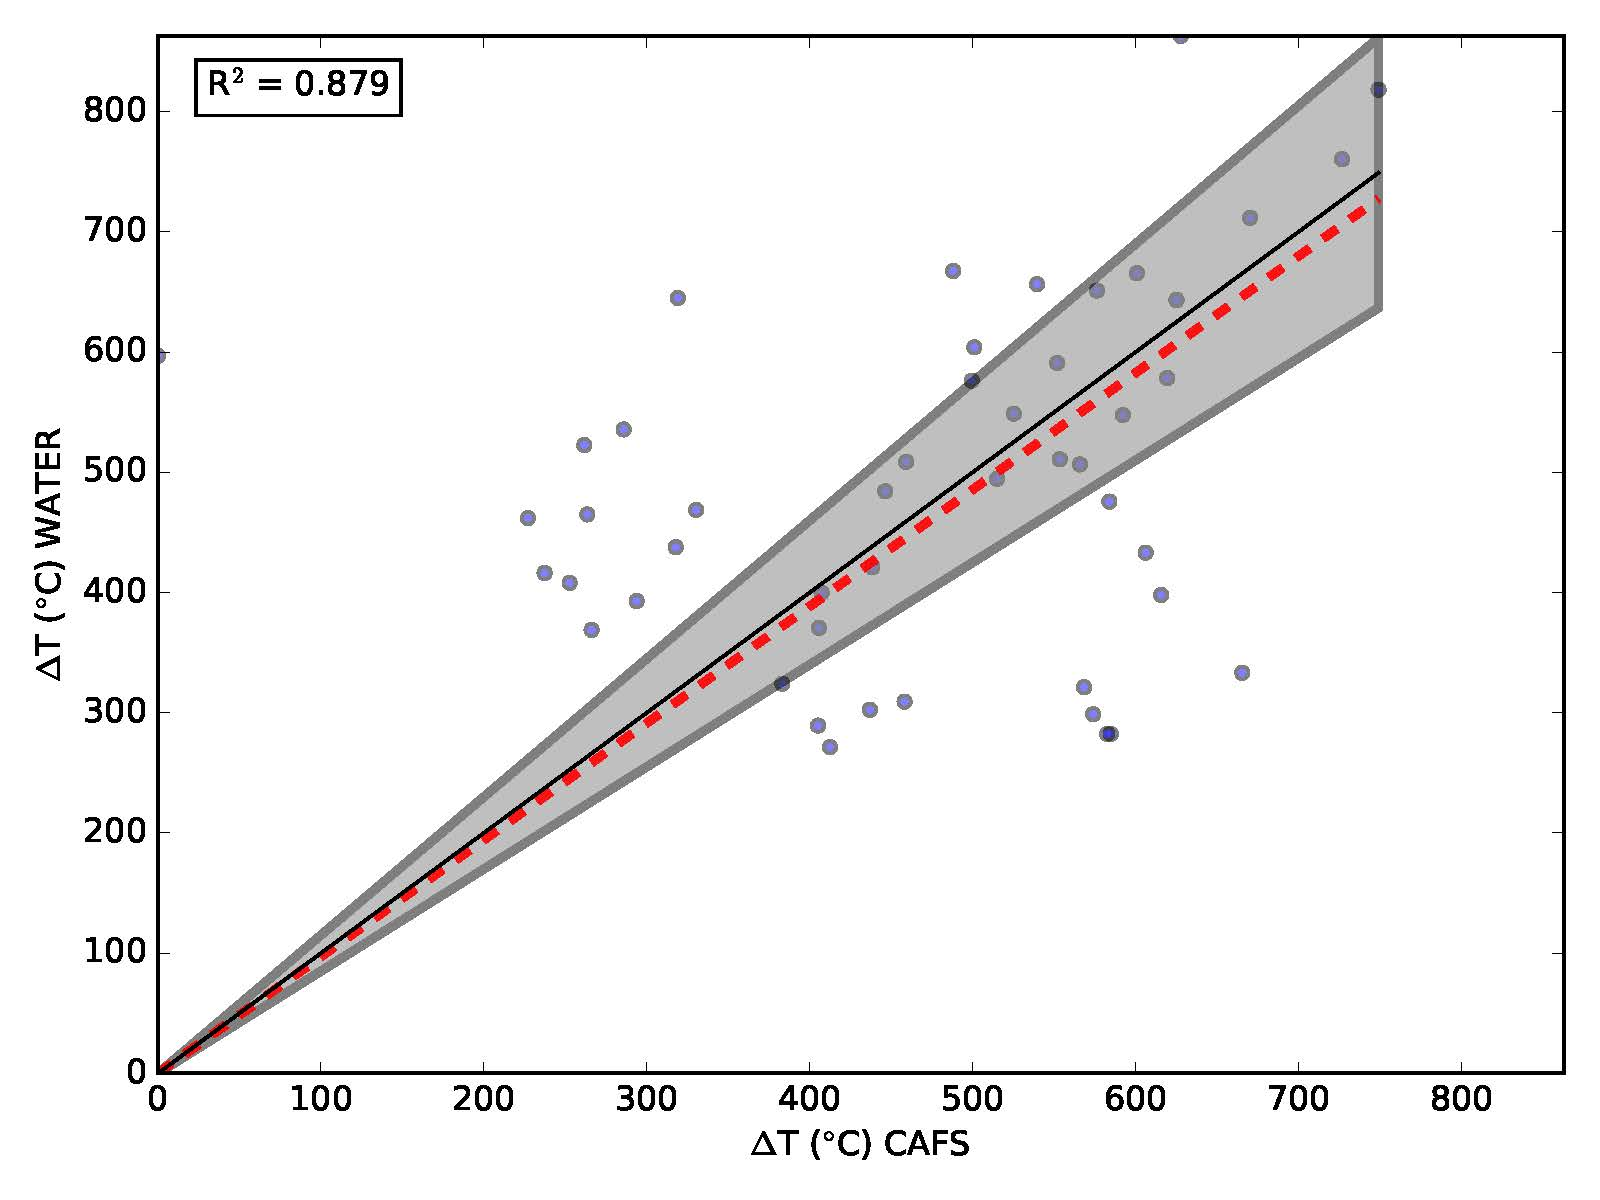
\includegraphics[width=.7\columnwidth]{../Figures/Script_Figures/TCA1_hallnozzle_scatter}
	\caption{CAF vs Water Temperature Difference Comparison for Single-Story Fire Suppression Tests at Thermocouple Array A1 after Hallway Nozzle}
	\label{fig:fs_hall_a1}
\end{figure}

\begin{figure}[!ht]
	\includegraphics[width=.7\columnwidth]{../Figures/Script_Figures/TCA1_doornozzle_scatter}
	\caption{CAF vs Water Temperature Difference Comparison for Single-Story Fire Suppression Tests at Thermocouple Array A1 after Door Nozzle}
	\label{fig:fs_door_a1}
\end{figure}

In Figure~\ref{fig:fs_hall_a1}, the red dashed line (linear fit to the data, see Section~\ref{sec:Gas_Cooling}) closely follows the black line, which indicates near equal cooling between CAF and water. The R$^2$ value of 0.879 shows a strong fit to the data. When the second nozzle (door nozzle) was activated, the temperature differences are noticeably lower compared to the hallway nozzle (indirect attack). While the fit is not as strong (R$^2$~=~0.643), the red line still falls within the experimental uncertainty, meaning that differences in the impact of CAF and water are indistinguishable. Despite being closer to the nozzles, thermocouple tree A2 shows similar temperature difference results from the hallway nozzle activation to the A1 array (see Figure~\ref{fig:fs_door_a2}). At array A2 for the door nozzle (see Figure~\ref{fig:fs_door_a2}), the red dashed falls outside of the experimental uncertainty, indicating a slight advantage of cooling for CAF.

\begin{figure}[!ht]
	\includegraphics[width=.7\columnwidth]{../Figures/Script_Figures/TCA2_hallnozzle_scatter}
	\caption{CAF vs Water Temperature Difference Comparison for Single-Story Fire Suppression Tests at Thermocouple Array A2 after Hallway Nozzle}
	\label{fig:fs_hall_a2}
\end{figure}

\begin{figure}[!ht]
	\includegraphics[width=.7\columnwidth]{../Figures/Script_Figures/TCA2_doornozzle_scatter}
	\caption{CAF vs Water Temperature Difference Comparison for Single-Story Fire Suppression Tests at Thermocouple Array A2 after Door Nozzle}
	\label{fig:fs_door_a2}
\end{figure}

\subsubsection*{Two-Story Structure}
\label{sec:fire_supp_two}

There were seven suppression tests conducted in the two-story, purpose-built structure. All seven of the tests used a fuel load consisting of three sofas, polypropylene carpeting over polyurethane foam padding, and OSB paneling along three walls and the ceiling. Five of the seven tests also had two stacks of wooden pallets in addition to the initial fuel load (Section~\ref{sec:fire_suppression_furniture_fuel}). Ignition occurred in the southwest corner of the ground floor and available ventilation was through the ground floor double doors and the door on the south side of the second story of the structure. The fires were intended to replicate room and contents basement fires typically seen within residential structures. Suppression occurred at the basement double doors of the structure. Table~\ref{tab:Test_Descriptions_2} provides an overview of the suppression tests conducted. In all cases, ventilation was provided through open basement doors and a door on the first floor.

\begin{table}[!ht]
\centering
\small
\caption{Two-Story Fire Suppression Test Descriptions}\label{tab:Test_Descriptions_2}
\begin{tabular}{cllll}
\toprule[1.5pt]
Test $\#$  & Name	& Stream			& Flow Rate		& Fuel                    \\
\midrule
 13  & CAF~7     &  Straight Stream  	&  120~gpm/60~cfm   & Furniture           \\
 14  & Water~7   &  Straight Stream  	&  120~gpm    		& Furniture           \\
 15  & CAF~8a    &  Straight Stream  	&  120~gpm/60~cfm   & Furniture + Pallet  \\
 16  & CAF~8b    &  Straight Stream  	&  120~gpm/60~cfm   & Furniture + Pallet  \\
 17  & Water~8   &  Straight Stream     &  120~gpm          & Furniture + Pallet  \\
 18  & Class A~1 &  Straight Stream  	&  120~gpm		    & Furniture + Pallet  \\
 19  & CAF~9a    &  1 3/8'' Ball    	&  120~gpm/60~cfm   & Furniture + Pallet  \\
 20  & CAF~9b    &  Solid Stream        &  120~gpm/60~cfm   & Furniture + Pallet  \\
\bottomrule[1.25pt]
\end{tabular}\par
\end{table}
  
Table~\ref{tab:Test_Results_2} provides the impact of suppression for the water, class A foam, and CAF tests conducted in the two-story structure. The measurement location was on the floor above the fire, at the doorway to the stairwell which connects the floors. The thermocouples at this measurement location were isolated from any direct contact from the suppression stream. The table provides the change in temperature 0.3~m (1~ft) below the ceiling and 0.3~m (1~ft) above the floor as well as the change in heat flux 1~m (3~ft) above the floor on the second floor level in front of the stairway door. Figure~\ref{fig:fire_supp_second_2story} shows the position of the thermocouple array (TC A10) as well as the three pairs of heat flux gauges. Table~\ref{tab:Test_Results_2} shows the heat flux at position 1, that faces in the vertical direction (toward the ceiling). Note that these thermocouples are inconel shielded thermocouples and have slower response times (smaller $\Delta$T's over similar time intervals) compared to the bare-bead thermocouples used in the single-story tests. The values reported in the table are immediately before and after the application period to assess the application agent, stream, and location on interior conditions.

\begin{table}[!ht]
\centering
\caption{Two-Story Fire Suppression Results, Stairwell Doorway Temperatures}\label{tab:Test_Results_2}
\begin{tabular}{lcccc}
\toprule[1.5pt]
           &               & \multicolumn{2}{c}{Temperature Change}                                    & Heat Flux Change \\
Test 	   & Flow Time (s) & 0.3~m Below Ceiling                 & 0.3~m Above Floor	               & 1~m Above Floor \\
\midrule
CAF~7      & 24            & 530~$^{\circ}$C - 425~$^{\circ}$C   & 670~$^{\circ}$C - 425~$^{\circ}$C   & 24~kW/m$^2$ - 17~kW/m$^2$  \\[.25cm]
Water~7    & 29            & 560~$^{\circ}$C - 430~$^{\circ}$C   & 670~$^{\circ}$C - 400~$^{\circ}$C   & 17~kW/m$^2$ - 17~kW/m$^2$  \\[.25cm]
CAF~8a     & 16            & 475~$^{\circ}$C - 425~$^{\circ}$C   & 580~$^{\circ}$C - 460~$^{\circ}$C   & 21~kW/m$^2$ - 14~kW/m$^2$  \\
CAF~8b     & 21            & 475~$^{\circ}$C - 400~$^{\circ}$C   & 540~$^{\circ}$C - 400~$^{\circ}$C   & 13~kW/m$^2$ - 12~kW/m$^2$  \\[.25cm]
Water~8    & 18            & 520~$^{\circ}$C - 460~$^{\circ}$C   & 530~$^{\circ}$C - 440~$^{\circ}$C   & 19~kW/m$^2$ - 14~kW/m$^2$  \\[.25cm]
Class A~1  & 19            & 470~$^{\circ}$C - 430~$^{\circ}$C   & 590~$^{\circ}$C - 500~$^{\circ}$C   & 13~kW/m$^2$ - 11~kW/m$^2$  \\
CAF~9a     & 21            & 530~$^{\circ}$C - 440~$^{\circ}$C   & 620~$^{\circ}$C - 450~$^{\circ}$C   & 17~kW/m$^2$ - 16~kW/m$^2$  \\
CAF~9b     & 16            & 580~$^{\circ}$C - 510~$^{\circ}$C   & 660~$^{\circ}$C - 525~$^{\circ}$C   & 20~kW/m$^2$ - 17~kW/m$^2$  \\
\bottomrule[1.25pt]
\end{tabular}\par
\end{table}

The time history profile of the temperature response along with the total heat flux at three positions is shown in Figures~\ref{fig:water7_tca10}--\ref{fig:caf9a_hf}. Figures~\ref{fig:water7_tca10} and \ref{fig:water7_hf} show the results for test Water~7, while Figures~\ref{fig:caf9a_tca10} and \ref{fig:caf9a_hf} show the results for test CAF~9a. The remainder of the fire suppression test data and results are included in Appendix~\ref{app:fire_suppression2}.

\begin{figure}[!ht]
	\includegraphics[width=.85\columnwidth]{../Figures/Script_Figures/Test_39_West_061315_TC_A10}
	\caption{Time Series of Thermocouple Data from Array TC A10 at the Top of the Stairwell for Two-Story Water~7 Fire Suppression Test}
	\label{fig:water7_tca10}
\end{figure}

\begin{figure}[!ht]
	\includegraphics[width=.85\columnwidth]{../Figures/Script_Figures/Test_39_West_061315_Heat_Flux}
	\caption{Time Series of Heat Flux Data at Three Locations on the Second Floor for Two-Story Water~7 Fire Suppression Test}
	\label{fig:water7_hf}
\end{figure}

\begin{figure}[!ht]
	\includegraphics[width=.85\columnwidth]{../Figures/Script_Figures/Test_41_West_061415_TC_A10}
	\caption{Time Series of Thermocouple Data from Array TC A10 at the Top of the Stairwell for Two-Story CAF~9a Fire Suppression Test}
	\label{fig:caf9a_tca10}
\end{figure}

\begin{figure}[!ht]
	\includegraphics[width=.85\columnwidth]{../Figures/Script_Figures/Test_41_West_061415_Heat_Flux}
	\caption{Time Series of Heat Flux Data at Three Locations on the Second Floor for Two-Story CAF~9a Fire Suppression Test}
	\label{fig:caf9a_hf}
\end{figure}

The impact of water and CAF during fire suppression can  again be analyzed by comparing the temperature differences during the suppression interval at the two thermocouple arrays in the fire room. Figure~\ref{fig:fs_a10} shows the temperature difference comparison at thermocouple array A10 for CAF and water after basement suppression. In Figure~\ref{fig:fs_a10}, only tests Water~7 \& 8 are compared to CAF~7 \& 8a as those are tests with comparable configurations.

\begin{figure}[!ht]
	\includegraphics[width=.7\columnwidth]{../Figures/Script_Figures/TC_A10_scatter}
	\caption{CAF vs Water Temperature Difference Comparison for Two-Story Fire Suppression Test at Thermocouple Array A10}
	\label{fig:fs_a10}
\end{figure}

In Figure~\ref{fig:fs_a10}, the red dashed line (linear fit to the data, see Section~\ref{sec:Gas_Cooling}) falls within the experimental uncertainty based around the equal cooling line (solid black line). This indicates an inability to distinguish whether CAF or water had a more significant impact in temperature reduction following suppression of the fire. The R$^2$ value of 0.975 shows a strong fit to the data between water and CAF. Similar to the single-story fire suppression tests, there are some differences in the changes in temperature and heat flux when comparing CAF to water, but the differences are not substantial. Both suppression agents had similar significant impact in reducing the high-temperature, high-heat flux environment that existed before suppression. 

\chapter{Discussion}
\label{chap:Discussion}

This study focused on two key types of fire experiments: gas cooling and fire suppression. In each type of experiment, a comparison was conducted between plain water and compressed air foam being discharged from nozzles of similar type with similar mass flow rates. In both types of experiments, there were no significant measurable differences between the use of plain water or compressed air foam. To expand upon the 2012 and 2013 tests described by Mitchell~\cite{Mitchell:1}, additional fire suppression experiments were conducted. One set of experiments used only wood-based fuels to examine the value of the reduced surface tension of the water in the CAF and its interaction with the surface of the wood fuel. A final experimental series was conducted in a larger fire room with more ventilation. In this final series, another change was made: the nozzle was hand held and could be moved as needed to effectively extinguish the fire. This section discusses the overall results of the study and provides potential explanations to support them.

\section{Gas Cooling}
\label{sec:Gas_Cooling_discuss}
 
Water is the most widely used fire extinguishing agent because it is effective, environmentally friendly, nontoxic, inexpensive, and in many cases, readily available. In addition, water has a very high heat of vaporization per unit mass, at least four times as high as that of any other nonflammable liquid~\cite{NFPA}. The latent heat of vaporization of water is 2255~kJ/kg (970~Btu/lb.)~\cite{NFPA}. This means that 2255~kJ (2139~Btu) of energy is required to change 1~kg (2.2~lb.) of water into steam. When water is vaporized, its volume increases approximately 1,700 times. Because the energy absorbing capabilities of water are well quantified, they can be used as a basis to calculate the theoretical minimum delivery rate of water needed to extinguish a burning material with a known heat (energy) release rate. Unfortunately, based on experience it has been estimated that water must be applied at 10 to 100 times the theoretical rate in order to control and extinguish the fire~\cite{Friedman:2}. As a result of this apparent inefficiency and the need to address fires containing a wide variety of materials, water-based fire fighting additives have been utilized for many years to enhance the fire fighting capabilities of ordinary water.

While CAF has been readily accepted for use in the wildland and wildland urban interface, the effectiveness or advantages of CAF for interior structural fire fighting was undocumented by experimental data. Questions remain regarding whether CAF provides improved gas cooling when compared to plain water. During the planning of the experiments for this project, there were a range of hypotheses regarding potential outcomes. Some technical panel members thought that the excellent heat absorbing capacity of plain water would exceed the heat absorbing capabilities of CAF. Their position was based on the fact that CAF has injected air. Because air is a great insulator, it slows heat transfer and results in less cooling. It was their belief that the reduced gas cooling capabilities of CAF may have led to firefighter injuries during interior fire attacks. Other members of the technical panel thought that the bubble structure would provide the same mass flow rate of water but with more surface area. The increased surface area would enable faster heat transfer rate and therefore improve the cooling of the hot gas layer. There were also thoughts that the CAFS would coat the ceiling and eliminate energy feedback from the ceiling to the hot gas layer, thereby providing enhanced cooling. However, CAF has not been widely used for structure fires.

The gas cooling experiments were designed to measure the ability of water streams and CAF streams to cool a hot gas layer without any application of agent to the source of the heat. The 3.35~m (11~ft) tall ceiling in the burn building allowed a hot gas layer of at least 1.83~m (6 ft) to form. During the testing, a minimum temperature of 250~$^{\circ}$C (482~$^{\circ}$F) at 1.83~m (6~ft) below the ceiling was attained prior to the beginning of gas cooling. In each gas cooling experiment, the same mass flow rate of water was used for both the plain water stream and the CAF stream. Typically, the volumetric flow rate of water was 7.57~L/s (120~gpm). The density of water is 1000~kg/m$^3$ (8.3~lb/gal), therefore the mass flow rate was 7.57~kg/s (16.7~lb/s). The average time of flow was approximately 15~s. A total of 114~kg (251~lb) of water was introduced into each gas cooling experiment.

When a CAF stream was used, it contained 0.3~\% foam concentration by volume. The density of the foam concentrate is 1055~kg/m$^3$ (8.8~lb/gal). For a 15~s flow time, 0.34~kg (0.75~lb) of concentrate was used. In addition to the foam concentrate and water, the CAF stream contained compressed air injected into the foam solution at a rate of 0.03~m$^3$/s (60~cfm). The density of the compressed air is in the range of 100 to 150~psig, which translates to a range between 8.9~kg/m$^3$ (0.6~lb/ft$^3$) and 12.8~kg/m$^3$ (0.8~lb/ft$^3$). Therefore, a 15~s CAF flow would contain approximately 4.0~kg (8.8~lb) to 9.5~kg (21.0~lb) of air. Comparing the mass flows and using the air mass based on the higher pressure, water still makes up more than 90~\% of the mass of the CAF stream.

The estimated total expanded uncertainty of the temperature measurements in these experiments is $\pm$~15~\% (see Section~\ref{subsec:Uncertainty}). For the difference between two temperature measurements to be considered significantly different, the difference would have to be greater by more than $\pm$~15~\%. If the difference between two measurements was $\pm$~15~\% or less, the results are considered similar. The estimated uncertainty is based on previous studies where suppression with a water based agent was included.

As mentioned in the results section, the conditions at TC Array 3 represented the ``best'' gas cooling results. It was impacted the least by agents hitting and cooling the thermocouples themselves. Under the given conditions of a residential scale room and the amount of water introduced into the hot gas layer, it should be no surprise that the water is absorbing the energy from the upper layer. Air filled bubbles in the CAF stream had no discernible impact, either positive or negative, in the gas cooling experiments. At the same time, there was no measurable negative effect of the air bubbles with regard to gas cooling.

The data from the thermocouples in TC Array 2 provide a sense of the impact of a combination of surface cooling and gas cooling. For example, when the nozzle was in the ``middle'' position, the straight or solid hose streams impacted the room's ceiling near the middle and created a fan pattern across the ceiling that caused the majority of the water to impact the location of TC Array 2 and the adjacent walls. In this location, the data tended to favor water. However, this did not represent gas cooling. Rather, this represented some of the water or CAF hitting the thermocouples and cooling the surrounding gases. As a result, temperature reductions of the thermocouples in TC Array 2 are higher than those of the thermocouples in TC Array 3, as shown in Figures~\ref{fig:CAFS_Water_A2_mid} and \ref{fig:CAFS_Water_A3_mid}, respectively.

TC Array 1 had the widest spread of temperature change. Depending on the nozzle configuration, there were tests where the thermocouples in TC Array 1 were directly impacted by water or CAF and other tests where there was no impact. Examination of the spray density figures in Appendix~\ref{app:spray_bb}, provides the range of agent collected in the bucket where TC Array 1 was located. In many cases, such as the test CAF Straight Stream Mid, the amount of foam solution collected was near zero. In other cases, such as the test CAF Fog Mid, the amount of foam solution collected was more than 3~kg (6.6~lb). Similar variations occurred with water. As a result, TC Array 1 did not provide consistent results for gas cooling.  

The data and results from this test series are not consistent with a hypothesis that firefighters were being injured during an interior fire fighting operation with CAF because CAF provided cooling similar to that of the equivalent flow rate of plain water.

\section{Fire Suppression}
\label{sec:Fire_Suppression_discussion}

Currently, the fire service uses ``fire flow'' formulas to estimate the flow rate of water needed to control a structure fire. The formulas are presented below and the results from the experiments described in this report will be compared with the calculated fire flows.

\subsection{Iowa State University Fire Flow Formula}
The Iowa Formula for determining the required fire flow rate for a given structure was developed by Keith Royer and Bill Nelson and is based on theoretical heat absorption capabilities of water \cite{Royer:ISU}. The required fire flow rate ($\dot{V}$) in gpm is equal to the volume ($V$) of the fire compartment in cubic feet divided by 100:

\begin{equation}\label{eq:isu_form}
\dot{V} = V / 100
\end{equation}

Due to inefficiencies in the application of water, some feel that the fire flow value from the Iowa State University formula should be multiplied by a factor of two to four~\cite{NFPA}. Applying the formula based on floor area yields an application density of 3.3~l/min/m$^2$ (0.08~gpm/ft$^2$) for ceiling heights of 2.44~m (8~ft) or 4.1~l/min/m$^2$ (0.10~gpm/ft$^2$) for ceiling heights of 3.05~m (10~ft). The fire room compartment volumes in these experiments ranged from approximately 66~m$^3$ (2330~ft$^3$) to 125~m$^3$ (4410~ft$^3$). The required flow rate for the fire room in the single-story structure based on the Iowa State University formula was approximately 87~l/min (23~gpm), and the required flow rate for the fire room in the lower level of the two-story structure was approximately 168~l/min (44~gpm). During the experiments, the flow rate was approximately 454~l/min (120~gpm), which exceeds the required flow rate of the Iowa State Formula. The fact that all of the fires were quickly controlled during the experiments is consistent with this methodology. 

\subsection{National Fire Academy}
The National Fire Academy (NFA) developed a formula based on a study of fire flows that have been successful in controlling a large number of working fires~\cite{Klaene:1}. This formula sets the required fire flow ($\dot{V}$) in gpm equal to the floor area ($A$) in square feet divided by 3.

\begin{equation}\label{eq:nfa_form}
\dot{V} = A / 3
\end{equation}

The fire rooms in these experiments ranged in floor area from approximately 27~m$^2$ (291~ft$^2$) to 51.4~m$^2$ (553~ft$^2$). Applying the NFA formula based on floor area yields a required flow rate for the single-story fire room of 369~l/min (97~gpm). The required flow rate for the fire room in the lower level of the two-story would be approximately 700~l/min (184~gpm). Comparing the hose stream flow rates to the NFA formula requirements indicates that 454~l/min (120~gpm) was sufficient for the smaller room fire in the single-story but was below the required flow rate of approximately 700~l/min (184~gpm) for the large fire compartment in the two-story structure. This is not consistent with the observations of a rapid fire knockdown with both water and CAF hose streams flowing 454~l/min (120~gpm). 

Due to recent research conducted by NIST and the UL Firefighter Safety Research Institute (FSRI), the fire service has a renewed interest in controlling the air available to a ventilation limited compartment fire. Limiting the air (oxygen) available for combustion is one means of limiting the heat release rate. If the heat release rate of a fire is reduced due to a lack of oxygen needed for combustion, then in theory, the amount of water needed to cool and suppress the fire should also be reduced.    

Both of the formulas listed above do not explicitly account for the ventilation of the fire structure, only the size of the fire structure. The most recent of the two formulas was developed in 1981, based on the fire ground experience of fire chiefs. This experience was likely from fires that occurred in the 1960's and the 1970's. It has been demonstrated that the synthetic fuels which fill the homes of the 2000's burn faster and with higher heat release rates than the natural fuels that filled the homes in the 1940's and 1950's. The change of materials in homes began in the 1960's and has continued to present day~\cite{Kerber:2}. It was unlikely, however, that this change was factored into the NFA formula.   

Shortly after the NFA equation was issued, another federal agency, the National Bureau of Standards (now NIST) released a finding about the relationship of oxygen to the heat release rate of a fire~\cite{Babrauskas:3}. NIST found that for many fuels, approximately 13.1~MJ of heat are generated for every kilogram of oxygen consumed during the combustion. This relationship led to simple algorithms that addressed the amount of oxygen that can flow through an opening with a theoretical heat release rate that assumes stoichiometric conditions (100~\% efficient burning where all of the fuel and the oxygen is consumed).

All of the fire conditions generated during these experiments were ventilation limited or ventilation controlled fires. Essentially, the conditions in the compartment were fuel rich. If the ventilation was increased to allow additional oxygen to be supplied to the fuel gases in the fire compartment, the heat release rate of the fire would have increased. There are simple formulas which may provide some insight here, although this simple algorithm has not been validated with the geometries that were used in the experiments described in this report. The purpose here is to estimate the amount of heat energy that the hose streams needed to overcome. This algorithm, like the NFA formula, has never been validated for this application. The heat release rate is: 

\begin{equation} \label{eq:HRRSto_item}
\dot{Q}_{stoichiometric} = 1500 A_0 \sqrt{H_0} \\
\end{equation}

In Equation~\ref{eq:HRRSto_item}, the maximum heat release rate ($\dot{Q}_{stoichiometric}$) in kW is based on airflow through the area of the opening ($A_0$) in square meters and the square root of the height of the opening ($H_0$) in meters.  

Following Equation~\ref{eq:HRRSto_item}, a single open doorway to a residential scale room that is approximately 0.9~m (3~ft) wide and 2.1~m (6.9~ft) high could support a heat release rate of approximately 4~MW, assuming complete combustion of the oxygen that would flow through the doorway opening via natural convection. For twice the width of the open doorway (the doorway on the lower level of the two-story structure), the theoretical heat release rate that could be supported inside the compartment would be approximately 8~MW. This does not account for flames burning outside of the compartment, which were frequently observed during testing.  

In the single-story structure, there was an additional window opening in some of the experiments which added ventilation to the room. In the two-story structure, there was an additional open doorway that allowed exhaust gases from the fire compartment to flow up the stairs, through the second-story floor, and out of the structure. Even with the additional ventilation in both cases, the conditions in the fire compartment remained fuel rich as the flames extended out of the structure's openings. Based on Equation~\ref{eq:HRRSto_item}, that would indicate that the heat release rate inside the compartment did not exceed 4~MW for the single-story structure or 8~MW for the two-story structure. 

Earlier, it was noted that the latent heat of vaporization of water is 2255~kJ/kg, or approximately 2.3~MJ/kg. Assuming ideal heat transfer, the mass flow rate of water needed to absorb the heat being generated inside the fire compartment would be approximately 1.8~kg/s for the single-story and 3.5~kg/s for the two-story. In these experiments, the mass flow rate of water was 7.57~kg/s (16.7~lb/s), which is theoretically twice what was needed to absorb the heat in the fire compartment of the larger fire in the lower level of the two-story structure. Again, this is a simplified analysis, much like the current tools provided in fire department literature for the required fire flow rate. However, it demonstrates that for a residential scale room (in this study up to to 51.4~m$^2$ (553~ft$^2$)) with the equivalent of two open doorways supplying fresh air, a flow of 2~gallons per second or 120~gpm of water was adequate to quickly suppress the fire in the compartment.                

In all the suppression experiments, the fire was controlled with a total flow of 227~L (60~gal) or less of agent. During the course of the suppression experiments, the fuel packages were modified to incorporate more wood-based fuels. During the planning of the experiments, some of the technical panel members felt that synthetic fuels, such as polyurethane foam, burned mostly at the surface and were therefore easily cooled and suppressed. Wood-based fuels, however, develop a char layer. The burning of wood-based fuels would be ``deep seated'', which might provide a more significant suppression challenge. The reduced surface tension of Class A foam solution could allow the solution to better penetrate and cool the burning wood-based fuels. It was thought that with more exposed burning wood surfaces in the fuel load, CAF would have a better the opportunity to demonstrate a difference in suppression. As shown in Section~\ref{sec:fuel_load}, the wood fuel load consisted of stacks of wood pallets, plywood lined walls, and an exposed wood ``ceiling'' that was constructed of wood ``i-beams'' and OSB. The experiments conducted with the wood fuel load did not demonstrate a significant difference between water and CAF.  

The final set of suppression experiments used a larger space than the previous two sets of suppression experiments in the single-story structure. As discussed previously, with the larger area and double the ventilation of the previous experiments, the fire should have been more challenging to the hose streams. There was also another variable that was be introduced: a firefighter controlling the nozzle. Recall that in the single-story experiments, a monitor nozzle was used in a fixed position. As a result, after the initial fire knockdown, it was typical that the agent was not able to hit all surface of the burning fuel sufficiently and a rekindle would occur. This can be seen for both the water and CAF experiments in the data provided in Appendix~\ref{app:fire_suppression}. In some single-story experiments, the fire was given time to redevelop and additional nozzle flows from the fixed positions were conducted to collect more data and to see if the fires could be extinguished. During the additional flows, no significant differences were seen. In all of the single-story experiments firefighters with a hoseline were needed to extinguish any remaining fire and hot spots. For the last set of experiments, the choice was made to use a firefighter so that the nozzle would be moved in an informed manner in order to make the best use of the hose stream to suppress the fire in the lower level of the two-story structure.  

The fire fighting crew was from the MCFRS and every member in the crew had been trained in the use of and had experience with using CAF. The firefighter on the nozzle was the same for all the experiments conducted in the two-story structure. The firefighter used the reach of the hose stream to cool the fire gases just inside the doorway as a means to knockdown the flames that were extending through the open double doors of the basement. Then, the hoseline was advanced and the nozzle was moved rapidly to hit the fuels inside the compartment. The nozzle was shut down when there were no flames visible from the doorway. The flow times were all less than 30 seconds. Even though the fire size had increased, a total flow of 227~L (60~gal) or less of agent was used to cool the hot gas layer and suppress each of the fires. This is consistent with the ventilation analysis above. The nozzle movement clearly had a positive impact on suppressing the fire in the 11~m (36~ft) deep fire compartment.    

During the workshop conducted for this project~\cite{Grant:2011}, it was suggested that CAF could suppress, or knockdown, a fire three to five times faster than water. The data collected during this study does not demonstrate significant differences between CAF and water for use in interior structural fire fighting on a residential scale. There is nothing in these fire suppression results to suggest that CAF would present a thermal hazard, provided that an adequate amount of water is being flowed for the given fire condition.

\section{Future Research}

One of the challenges with suppression research or determining the required flow rate of water needed on a building fire is the lack of data on realistic baseline requirements of the total amount of water needed for gas cooling and suppression. In this study, the data demonstrates that there was a sufficient amount of water for gas cooling and suppression. One question that arises is, how much could the flow rate of water have been reduced before a significant difference in performance was observed? 

Information from actual incidents in the field shaped this study. From the gas cooling and suppression perspective, the results did not demonstrate significant differences between plain water and CAF. However, there are other issues like nozzle reaction force and flow separation which have been covered in the Cal Poly fire ground studies that can be addressed in training~\cite{Carracino:2013,Dicus:2013,LaPolla:2012}.  It is important to provide adequate training when adopting a new method or new technology. These types of issues should be examined further to better understand how suppression activities take place in the field.

Additional research is needed to examine the impact of nozzle type and nozzle movement on the fire environment. It is possible that some of the discomfort or injuries that firefighters experience during interior fire fighting could be the result of a poor choice of nozzle or nozzle movement that results in displacing hotter gases into the area where the firefighter is located. Currently, the fire service relies on experience to develop a feel for the correct combination of nozzle type and movement. A study may be able to demonstrate a clear cause and effect relationship between the amount of water flowing, the type of nozzle, and the movement of the nozzle and how such choices can impact the flow of gases within the structure. Based on the results of this study, it appears that training and understanding the impact of nozzle movement may be potential paths to more effective use of water. 

\chapter{Summary}
\label{chap:Summary}

This study conducted by NIST was part of a larger research project led by California Polytechnic State University (Cal Poly), San Luis Obispo in collaboration with the Montgomery County (MD) Fire and Rescue Service. This study was supported in part by a DHS/FEMA Assistance to Firefighters Research and Development Grant.  

Experiments were conducted to investigate the capabilities and limitations of compressed air foam (CAF) relative to water when used for interior structural fire fighting in residential structures. The experimental designs were developed based on a project planning workshop led by the Fire Protection Research Foundation~\cite{Grant:2011}. The key outcomes were to measure the gas cooling and fire suppression capabilities of CAF compared to water. Incidents where firefighters had experienced burn injuries or other challenges while using CAF during interior attack operations in residential occupancies served as the catalyst for this study.

Full-scale fire experiments designed to address those questions were conducted over a period of years from 2012 through 2015. The experimental configurations were designed to be representative of residential fire scenarios. %The water and CAF flows were based on those used by a fire department with 35 CAFS front line engines. This same department also experienced injuries to firefighters while using CAF during interior fire fighting operations in residential structures. 
This study was composed of three types of experiments: spray density, gas cooling, and fire suppression. In each type of experiment, a comparison was conducted between plain water and CAF being discharged from nozzles of similar types with similar mass flow rates of water. The flow rate for each water experiment was 120~gpm. For the CAF experiments, 60~cfm of air and a 0.3~\% flow of Class A foam concentrate were added to the water flow.

Thirty-two spray density tests were conducted to determine where the suppression agent would land within a compartment based on various nozzle patterns and locations. The gas cooling and fire suppression tests simulated an interior fire attack through the deployment of hose lines inside the structures with fixed nozzles. The purpose of these spray density tests was to determine the appropriate nozzle locations for the gas cooling and fire suppression tests by gaining an understanding of the water distribution throughout the structures. This report provides a complete set of the spray density results in graphic form.

Eighty-eight gas cooling experiments were conducted to study the effectiveness of cooling the upper gas layer in a space adjacent to the area of fire involvement. These tests examined five different hose stream patterns, two nozzle types, and both compressed air foam and water as the suppression agent. The focus of this experimental series was to study the impact of the test variables on the hot gas layer temperatures when a fixed hose stream was applied to a room adjacent to the fire room. Suppression agents were not applied to the fire in the burn room. In this report, an aggregate analysis was made to examine differences due to the location of the instrumentation relative to the impact area of the agent and compare the differences in the amount of gas cooling between plain water and CAF hose streams. The results showed that water was generally more effective than CAF, though both agents were successful with respect to gas cooling and fire suppression. A more detailed analysis of the individual experiments was conducted by Mitchell of Cal Poly~\cite{Mitchell:1}. The conclusion of both analyses is in agreement. The full gas cooling data set can be found in the Mitchell report.    

There were two different geometries used for the fire suppression experiments. Twelve of the suppression experiments were conducted in a single-story structure with an entry hallway that led to a fire compartment with a floor area of 27~m$^2$ (291~ft$^2$). Within this structure, two different types of fuel loads were used. In one case, most of the fuel consisted of synthetic materials in the upholstered furniture, carpet, and padding. The other fuel load used only wood-based fuels to examine the value of the reduced surface tension of the water in the CAF and its interaction with the surface of the wood fuel. In the experiments conducted in the single-story building, a fixed nozzle was flowed from the hallway for approximately 15~s, and then another fixed nozzle located in the fire compartment was flowed for an additional 15~s.   

Seven of the suppression experiments were conducted in a two-story structure.  The fire compartment was the full lower level of the structure, and it had an open floor plan with an area of 51.4~m$^2$ (553~ft$^2$). At one end of the room was an open doorway that was 1.8~m (6~ft) wide and 2~m (6.7~ft) high and led to a stairwell. A manual hose stream application was made from outside the doorway on the lower level. In these experiments, there was a combination of wood-based and synthetic fuels. The fires were allowed to transition through flashover and then the initial fire suppression attack was made. In each case, the initial knockdown of the fire required 60~gal of agent or less.   

The results from both the gas cooling and the suppression of residential scale room fires showed the effectiveness of water and CAF hose streams to be similar. Under these test conditions both agents were effective. This study did not address the previously documented attributes of CAF for improved exposure protection and improved prevention of a fire re-kindle relative to plain water. 


\chapter{Acknowledgments}
\label{chap:acknowledgments}

The authors would like to thank Roy McLane (currently with Thermal Fabrication), Kristopher Overholt (currently with Continuum Analytics), Adam Barowy (currently with UL), Kelly Opert (currently with UL) and Jay McElroy (retired) from NIST for their contributions in preparing and conducting these experiments. These experiments could not have been conducted without them. 

Thank you to Chief Scott Goldstein and former Chief Steve Lohr of the Montgomery County (MD) Fire and Rescue Service for their support of this study. The authors would also like to thank the Montgomery County (MD) firefighters that supported the experiments: Alan Butsch, Daniel Hudson, Michael Johns, Steven Neubauer, Curtis Poole, Sean Regan, Chris Reilly, Bryan Rojtas, Ralph Thomas, and Douglas Wallace. 

The NIST team would like to thank Casey Grant from the Fire Protection Research Foundation and the members of the project technical panel, especially John Culbertson, Director, Montana State University Fire Services Training School and Homer Robertson, Deputy Chief, Fort Worth Fire Department.  

The Delaware County Emergency Services Training Center provided the location and logistical support for these experiments. The Delaware County team was under the direction of Kerby Kerber.  The construction and test support team included: Joe Bingham, Dave Wright, Dave Nercesian (small engine repair), Mike Gura, Scott Wiercinski, Bill Fields (Fields Fire Protection), John Hale and Todd John.

Thanks are given to the dedicated team of fire instructors and firefighters that supported these experiments; Brian Righter (Rudy), John McGowan, Matthew Poissant, John Frey, Brian Embert, Raymond Keller III, Mike Bramble, Edward McBride, Mark Morrissey, Bill Norris, and Matt LeTourneau.

Thanks to all involved for assisting in generating data that will aid the fire service in making evidence based tactical choices.

\bibliography{../../../Bibliography/FDS_refs,../../../Bibliography/FDS_general}

\appendix

\chapter{Dimensioned Floor Plans}
\label{app:floor_plans}

\begin{figure}[!ht]
	\includegraphics[width=\columnwidth]{../Figures/Floor_Plans/PDFs/West_Structure/DelCo_2012_West_Structure_Detailed}
	\caption{Fully Dimensioned Floor Plan of the Burn Building Layout}
	\label{fig:Delaware_County,_PA_Burn_Building_Layout_Detailed}
\end{figure}

\begin{figure}[!ht]
	\includegraphics[width=\columnwidth]{../Figures/Floor_Plans/PDFs/East_Structure/DelCo_2012_East_Structure_Detailed}
	\caption{Fully Dimensioned Floor Plan of the Single-Story Test Structure}
	\label{fig:Test_Structure_Floor_Plan_Detailed}
\end{figure}

\clearpage

\begin{figure}[!ht]
	\includegraphics[width=\columnwidth]{../../DelCo_2014_2015/Drawings/PDFs/CAFS/West_Structure_1st_Floor_Plain}
	\caption{Fully Dimensioned Floor Plan of the First Floor of the Two-Story Structure}
	\label{fig:dimensioned_first_2story_detailed}
\end{figure}

\begin{figure}[!ht]
	\includegraphics[width=\columnwidth]{../../DelCo_2014_2015/Drawings/PDFs/CAFS/West_Structure_2nd_Floor_Plain}
	\caption{Fully Dimensioned Floor Plan of the Second Floor of the Two-Story Structure}
	\label{fig:dimensioned_second_2story_detailed}
\end{figure}


\chapter{Spray Density Figures}
\label{app:spray_density}

\section{Spray density figures for burn building tests}
\label{app:spray_bb}

\begin{figure}[ht]
\begin{tabular*}{\textwidth}{lr}
\includegraphics[width=3.2in]{../Figures/Bars/BB1} &
\includegraphics[width=3.2in]{../Figures/Bars/BB2} \\
\includegraphics[width=3.2in]{../Figures/Bars/BB3} &
\includegraphics[width=3.2in]{../Figures/Bars/BB4}
\end{tabular*}
\caption{Spray density figures for burn building tests 1) Water Straight Stream Back (upper left), 2) Water Straight Stream Back (upper right), 3) Water Straight Stream Mid (lower left), and 4) Water Straight Stream Mid (lower right)}
\label{fig:bb_1_4}
\end{figure}

\clearpage

\begin{figure}[ht]
\begin{tabular*}{\textwidth}{lr}
\includegraphics[width=3.2in]{../Figures/Bars/BB5} &
\includegraphics[width=3.2in]{../Figures/Bars/BB6} \\
\includegraphics[width=3.2in]{../Figures/Bars/BB7} &
\includegraphics[width=3.2in]{../Figures/Bars/BB8}
\end{tabular*}
\caption{Spray density figures for burn building tests 5) Water Straight Stream Mid (upper left), 6) Water Fog Mid (upper right), 7) Water Fog Mid (lower left), and 8) Water Fog Back (lower right)}
\label{fig:bb_5_8}
\end{figure}

\clearpage

\begin{figure}[ht]
\begin{tabular*}{\textwidth}{lr}
\includegraphics[width=3.2in]{../Figures/Bars/BB9} &
\includegraphics[width=3.2in]{../Figures/Bars/BB10} \\
\includegraphics[width=3.2in]{../Figures/Bars/BB11} &
\includegraphics[width=3.2in]{../Figures/Bars/BB12}
\end{tabular*}
\caption{Spray density figures for burn building tests 9) Water Fog Back (upper left), 10) Water Solid Stream Back (upper right), 11) Water Solid Stream Back (lower left), and 12) CAF Solid Stream Back (lower right)}
\label{fig:bb_9_12}
\end{figure}

\clearpage

\begin{figure}[ht]
\begin{tabular*}{\textwidth}{lr}
\includegraphics[width=3.2in]{../Figures/Bars/BB13} &
\includegraphics[width=3.2in]{../Figures/Bars/BB14} \\
\includegraphics[width=3.2in]{../Figures/Bars/BB15} &
\includegraphics[width=3.2in]{../Figures/Bars/BB16}
\end{tabular*}
\caption{Spray density figures for burn building tests 13) CAF Solid Stream Mid (upper left), 14) CAF Solid Stream Back (upper right), 15) CAF Solid Stream Mid (lower left), and 16) CAF Fog Mid (lower right)}
\label{fig:bb_13_16}
\end{figure}

\clearpage

\begin{figure}[ht]
\begin{tabular*}{\textwidth}{lr}
\includegraphics[width=3.2in]{../Figures/Bars/BB17} &
\includegraphics[width=3.2in]{../Figures/Bars/BB18} \\
\includegraphics[width=3.2in]{../Figures/Bars/BB19} &
\includegraphics[width=3.2in]{../Figures/Bars/BB20}
\end{tabular*}
\caption{Spray density figures for burn building tests 17) CAF Straight Stream Mid (upper left), 18) CAF Straight Stream Mid (upper right), 19) CAF Fog Back (lower left), and 20) CAF Fog Back (lower right)}
\label{fig:bb_19_21}
\end{figure}

\clearpage

\begin{figure}[ht]
\centering
\includegraphics[width=3.2in]{../Figures/Bars/BB21}
\caption{Spray density figures for burn building test 21) CAF Straight Stream Back}
\label{fig:bb_21}
\end{figure}

\clearpage

\section{Spray density figures for experimental structure tests}
\label{app:spray_es}

\begin{figure}[ht]
\begin{tabular*}{\textwidth}{lr}
\includegraphics[width=3.2in]{../Figures/Bars/ES_1} &
\includegraphics[width=3.2in]{../Figures/Bars/ES_2} \\
\includegraphics[width=3.2in]{../Figures/Bars/ES_3} &
\includegraphics[width=3.2in]{../Figures/Bars/ES_4}
\end{tabular*}
\caption{Spray density figures for experimental structure tests 1) Water Straight Stream FR (upper left), 2) Water Straight Stream FR (upper right), 3) Water Straight Stream FR (lower left), and 4) Water Straight Stream FR (lower right)}
\label{fig:es_1_4}
\end{figure}

\clearpage

\begin{figure}[ht]
\begin{tabular*}{\textwidth}{lr}
\includegraphics[width=3.2in]{../Figures/Bars/ES_5} &
\includegraphics[width=3.2in]{../Figures/Bars/ES_6} \\
\includegraphics[width=3.2in]{../Figures/Bars/ES_7} &
\includegraphics[width=3.2in]{../Figures/Bars/ES_72}
\end{tabular*}
\caption{Spray density figures for experimental structure tests 5) Water Fog FR (upper left), 6) Water Fog FR (upper right), 7) Water Solid Stream FR (lower left), and 8) Water Solid Stream H (lower right)}
\label{fig:es_5_72}
\end{figure}

\clearpage

\begin{figure}[ht]
\begin{tabular*}{\textwidth}{lr}
\includegraphics[width=3.2in]{../Figures/Bars/ES_8} &
\includegraphics[width=3.2in]{../Figures/Bars/ES_9} \\
\includegraphics[width=3.2in]{../Figures/Bars/ES_10} &
\includegraphics[width=3.2in]{../Figures/Bars/ES_11}
\end{tabular*}
\caption{Spray density figures for experimental structure tests 9) Water Fog H (upper left), 10) Water Fog H (upper right), 11) Water Straight Stream H (lower left), and 12) Water Straight Stream H (lower right)}
\label{fig:es_8_11}
\end{figure}

\chapter{Single-Story Fire Suppression Data}
\label{app:fire_suppression}
\newpage

\begin{figure}[ht]
\includegraphics[width=.725\columnwidth]{../Figures/Script_Figures/FSE_Test_1_092812_TC_A1}
\includegraphics[width=.725\columnwidth]{../Figures/Script_Figures/FSE_Test_1_092812_TC_A2}
\includegraphics[width=.725\columnwidth]{../Figures/Script_Figures/FSE_Test_1_092812_TC_A3}
\caption{Thermocouple Data for Arrays in the Fire Room (top - A1, middle - A2) and in the Hallway (bottom - A3) for Single-Story Fire Suppression Test CAF~1}
\end{figure}


\begin{figure}[ht]
\includegraphics[width=.725\columnwidth]{../Figures/Script_Figures/FSE_Test_1_092812_Heat_Flux_1}
\includegraphics[width=.725\columnwidth]{../Figures/Script_Figures/FSE_Test_1_092812_Heat_Flux_3}
\caption{Heat Flux and Radiometer Data in the Fire Room (top - 1/2) and in the Hallway (bottom - 3/4) for Single-Story Fire Suppression Test CAF~1}
\end{figure}

\begin{figure}[ht]
\includegraphics[width=.725\columnwidth]{../Figures/Script_Figures/FSE_Test_1_092812_BDP_A3}
\caption{Hallway Velocity Data from Bi-Directional Probes for Single-Story Fire Suppression Test CAF~1}
\end{figure}

\begin{figure}[ht]
\includegraphics[width=.725\columnwidth]{../Figures/Script_Figures/FSW_Test_2_092812_TC_A1}
\includegraphics[width=.725\columnwidth]{../Figures/Script_Figures/FSW_Test_2_092812_TC_A2}
\includegraphics[width=.725\columnwidth]{../Figures/Script_Figures/FSW_Test_2_092812_TC_A3}
\caption{Thermocouple Data for Arrays in the Fire Room (top - A1, middle - A2) and in the Hallway (bottom - A3) for Single-Story Fire Suppression Test Water~1}
\end{figure}

\begin{figure}[ht]
\includegraphics[width=.725\columnwidth]{../Figures/Script_Figures/FSW_Test_2_092812_Heat_Flux_1}
\includegraphics[width=.725\columnwidth]{../Figures/Script_Figures/FSW_Test_2_092812_Heat_Flux_3}
\caption{Heat Flux and Radiometer Data in the Fire Room (top - 1/2) and in the Hallway (bottom - 3/4) for Single-Story Fire Suppression Test Water~1}
\end{figure}

\begin{figure}[ht]
\includegraphics[width=.725\columnwidth]{../Figures/Script_Figures/FSW_Test_2_092812_BDP_A3}
\caption{Hallway Velocity Data from Bi-Directional Probes for Single-Story Fire Suppression Test Water~1}
\end{figure}

\begin{figure}[ht]
\includegraphics[width=.725\columnwidth]{../Figures/Script_Figures/FSW_Test_3_092812_TC_A1}
\includegraphics[width=.725\columnwidth]{../Figures/Script_Figures/FSW_Test_3_092812_TC_A2}
\includegraphics[width=.725\columnwidth]{../Figures/Script_Figures/FSW_Test_3_092812_TC_A3}
\caption{Thermocouple Data for Arrays in the Fire Room (top - A1, middle - A2) and in the Hallway (bottom - A3) for Single-Story Fire Suppression Test CAF~2}
\end{figure}

\begin{figure}[ht]
\includegraphics[width=.725\columnwidth]{../Figures/Script_Figures/FSW_Test_3_092812_Heat_Flux_1}
\includegraphics[width=.725\columnwidth]{../Figures/Script_Figures/FSW_Test_3_092812_Heat_Flux_3}
\caption{Heat Flux and Radiometer Data in the Fire Room (top - 1/2) and in the Hallway (bottom - 3/4) for Single-Story Fire Suppression Test CAF~2}
\end{figure}

\begin{figure}[ht]
\includegraphics[width=.725\columnwidth]{../Figures/Script_Figures/FSW_Test_3_092812_BDP_A3}
\caption{Hallway Velocity Data from Bi-Directional Probes for Single-Story Fire Suppression Test CAF~2}
\end{figure}

\begin{figure}[ht]
\includegraphics[width=.725\columnwidth]{../Figures/Script_Figures/FSE_Test_4_092912_TC_A1}
\includegraphics[width=.725\columnwidth]{../Figures/Script_Figures/FSE_Test_4_092912_TC_A2}
\includegraphics[width=.725\columnwidth]{../Figures/Script_Figures/FSE_Test_4_092912_TC_A3}
\caption{Thermocouple Data for Arrays in the Fire Room (top - A1, middle - A2) and in the Hallway (bottom - A3) for Single-Story Fire Suppression Test Water~2}
\end{figure}

\begin{figure}[ht]
\includegraphics[width=.725\columnwidth]{../Figures/Script_Figures/FSE_Test_4_092912_Heat_Flux_1}
\includegraphics[width=.725\columnwidth]{../Figures/Script_Figures/FSE_Test_4_092912_Heat_Flux_3}
\caption{Heat Flux and Radiometer Data in the Fire Room (top - 1/2) and in the Hallway (bottom - 3/4) for Single-Story Fire Suppression Test Water~2}
\end{figure}

\begin{figure}[ht]
\includegraphics[width=.725\columnwidth]{../Figures/Script_Figures/FSE_Test_4_092912_BDP_A3}
\caption{Hallway Velocity Data from Bi-Directional Probes for Single-Story Fire Suppression Test Water~2}
\end{figure}

\begin{figure}[ht]
\includegraphics[width=.725\columnwidth]{../Figures/Script_Figures/FSW_Test_6_093012_TC_A1}
\includegraphics[width=.725\columnwidth]{../Figures/Script_Figures/FSW_Test_6_093012_TC_A2}
\includegraphics[width=.725\columnwidth]{../Figures/Script_Figures/FSW_Test_6_093012_TC_A3}
\caption{Thermocouple Data for Arrays in the Fire Room (top - A1, middle - A2) and in the Hallway (bottom - A3) for Single-Story Fire Suppression Test CAF~3}
\end{figure}

\begin{figure}[ht]
\includegraphics[width=.725\columnwidth]{../Figures/Script_Figures/FSW_Test_6_093012_Heat_Flux_1}
\includegraphics[width=.725\columnwidth]{../Figures/Script_Figures/FSW_Test_6_093012_Heat_Flux_3}
\caption{Heat Flux and Radiometer Data in the Fire Room (top - 1/2) and in the Hallway (bottom - 3/4) for Single-Story Fire Suppression Test CAF~3}
\end{figure}

\begin{figure}[ht]
\includegraphics[width=.725\columnwidth]{../Figures/Script_Figures/FSW_Test_6_093012_BDP_A3}
\caption{Hallway Velocity Data from Bi-Directional Probes for Single-Story Fire Suppression Test CAF~3}
\end{figure}

\begin{figure}[ht]
\includegraphics[width=.725\columnwidth]{../Figures/Script_Figures/FSE_Test_5_093912_TC_A1}
\includegraphics[width=.725\columnwidth]{../Figures/Script_Figures/FSE_Test_5_093912_TC_A2}
\includegraphics[width=.725\columnwidth]{../Figures/Script_Figures/FSE_Test_5_093912_TC_A3}
\caption{Thermocouple Data for Arrays in the Fire Room (top - A1, middle - A2) and in the Hallway (bottom - A3) for Single-Story Fire Suppression Test Water~3}
\end{figure}

\begin{figure}[ht]
\includegraphics[width=.725\columnwidth]{../Figures/Script_Figures/FSE_Test_5_093912_Heat_Flux_1}
\includegraphics[width=.725\columnwidth]{../Figures/Script_Figures/FSE_Test_5_093912_Heat_Flux_3}
\caption{Heat Flux and Radiometer Data in the Fire Room (top - 1/2) and in the Hallway (bottom - 3/4) for Single-Story Fire Suppression Test Water~3}
\end{figure}

\clearpage

\begin{figure}[ht]
\includegraphics[width=.725\columnwidth]{../Figures/Script_Figures/FSE_Test_5_093912_BDP_A3}
\caption{Hallway Velocity Data from Bi-Directional Probes for Single-Story Fire Suppression Test Water~3}
\end{figure}

\begin{figure}[ht]
\includegraphics[width=.725\columnwidth]{../Figures/Script_Figures/FSE_Test_8_093912_TC_A1}
\includegraphics[width=.725\columnwidth]{../Figures/Script_Figures/FSE_Test_8_093912_TC_A2}
\includegraphics[width=.725\columnwidth]{../Figures/Script_Figures/FSE_Test_8_093912_TC_A3}
\caption{Thermocouple Data for Arrays in the Fire Room (top - A1, middle - A2) and in the Hallway (bottom - A3) for Single-Story Fire Suppression Test CAF~4}
\end{figure}

\begin{figure}[ht]
\includegraphics[width=.725\columnwidth]{../Figures/Script_Figures/FSE_Test_8_093912_Heat_Flux_1}
\includegraphics[width=.725\columnwidth]{../Figures/Script_Figures/FSE_Test_8_093912_Heat_Flux_3}
\caption{Heat Flux and Radiometer Data in the Fire Room (top - 1/2) and in the Hallway (bottom - 3/4) for Single-Story Fire Suppression Test CAF~4}
\end{figure}

\begin{figure}[ht]
\includegraphics[width=.725\columnwidth]{../Figures/Script_Figures/FSE_Test_8_093912_BDP_A3}
\caption{Hallway Velocity Data from Bi-Directional Probes for Single-Story Fire Suppression Test CAF~4}
\end{figure}

\begin{figure}[ht]
\includegraphics[width=.725\columnwidth]{../Figures/Script_Figures/FSW_Test_7_093012_TC_A1}
\includegraphics[width=.725\columnwidth]{../Figures/Script_Figures/FSW_Test_7_093012_TC_A2}
\includegraphics[width=.725\columnwidth]{../Figures/Script_Figures/FSW_Test_7_093012_TC_A3}
\caption{Thermocouple Data for Arrays in the Fire Room (top - A1, middle - A2) and in the Hallway (bottom - A3) for Single-Story Fire Suppression Test Water~4}
\end{figure}

\begin{figure}[ht]
\includegraphics[width=.725\columnwidth]{../Figures/Script_Figures/FSW_Test_7_093012_Heat_Flux_1}
\includegraphics[width=.725\columnwidth]{../Figures/Script_Figures/FSW_Test_7_093012_Heat_Flux_3}
\caption{Heat Flux and Radiometer Data in the Fire Room (top - 1/2) and in the Hallway (bottom - 3/4) for Single-Story Fire Suppression Test Water~4}
\end{figure}

\begin{figure}[ht]
\includegraphics[width=.725\columnwidth]{../Figures/Script_Figures/FSW_Test_7_093012_BDP_A3}
\caption{Hallway Velocity Data from Bi-Directional Probes for Single-Story Fire Suppression Test Water~4}
\end{figure}

\begin{figure}[ht]
\includegraphics[width=.725\columnwidth]{../Figures/Script_Figures/FSW_Test_12_051613_TC_A1}
\includegraphics[width=.725\columnwidth]{../Figures/Script_Figures/FSW_Test_12_051613_TC_A2}
\includegraphics[width=.725\columnwidth]{../Figures/Script_Figures/FSW_Test_12_051613_TC_A3}
\caption{Thermocouple Data for Arrays in the Fire Room (top - A1, middle - A2) and in the Hallway (bottom - A3) for Single-Story Fire Suppression Test CAF~5}
\end{figure}

\begin{figure}[ht]
\includegraphics[width=.725\columnwidth]{../Figures/Script_Figures/FSW_Test_12_051613_Heat_Flux_1}
\includegraphics[width=.725\columnwidth]{../Figures/Script_Figures/FSW_Test_12_051613_Heat_Flux_3}
\caption{Heat Flux and Radiometer Data in the Fire Room (top - 1/2) and in the Hallway (bottom - 3/4) for Single-Story Fire Suppression Test CAF~5}
\end{figure}

\begin{figure}[ht]
\includegraphics[width=.725\columnwidth]{../Figures/Script_Figures/FSW_Test_12_051613_BDP_A3}
\caption{Hallway Velocity Data from Bi-Directional Probes for Single-Story Fire Suppression Test CAF~5}
\end{figure}

\begin{figure}[ht]
\includegraphics[width=.725\columnwidth]{../Figures/Script_Figures/FSE_Test_11_051613_TC_A1}
\includegraphics[width=.725\columnwidth]{../Figures/Script_Figures/FSE_Test_11_051613_TC_A2}
\includegraphics[width=.725\columnwidth]{../Figures/Script_Figures/FSE_Test_11_051613_TC_A3}
\caption{Thermocouple Data for Arrays in the Fire Room (top - A1, middle - A2) and in the Hallway (bottom - A3) for Single-Story Fire Suppression Test Water~5}
\end{figure}

\begin{figure}[ht]
\includegraphics[width=.725\columnwidth]{../Figures/Script_Figures/FSE_Test_11_051613_Heat_Flux_1}
\includegraphics[width=.725\columnwidth]{../Figures/Script_Figures/FSE_Test_11_051613_Heat_Flux_3}
\caption{Heat Flux and Radiometer Data in the Fire Room (top - 1/2) and in the Hallway (bottom - 3/4) for Single-Story Fire Suppression Test Water~5}
\end{figure}

\begin{figure}[ht]
\includegraphics[width=.725\columnwidth]{../Figures/Script_Figures/FSE_Test_11_051613_BDP_A3}
\caption{Hallway Velocity Data from Bi-Directional Probes for Single-Story Fire Suppression Test Water~5}
\end{figure}

\begin{figure}[ht]
\includegraphics[width=.725\columnwidth]{../Figures/Script_Figures/FSW_Test_14_052013_TC_A1}
\includegraphics[width=.725\columnwidth]{../Figures/Script_Figures/FSW_Test_14_052013_TC_A2}
\includegraphics[width=.725\columnwidth]{../Figures/Script_Figures/FSW_Test_14_052013_TC_A3}
\caption{Thermocouple Data for Arrays in the Fire Room (top - A1, middle - A2) and in the Hallway (bottom - A3) for Single-Story Fire Suppression Test CAF~6}
\end{figure}

\begin{figure}[ht]
\includegraphics[width=.725\columnwidth]{../Figures/Script_Figures/FSW_Test_14_052013_Heat_Flux_1}
\includegraphics[width=.725\columnwidth]{../Figures/Script_Figures/FSW_Test_14_052013_Heat_Flux_3}
\caption{Heat Flux and Radiometer Data in the Fire Room (top - 1/2) and in the Hallway (bottom - 3/4) for Single-Story Fire Suppression Test CAF~6}
\end{figure}

\begin{figure}[ht]
\includegraphics[width=.725\columnwidth]{../Figures/Script_Figures/FSW_Test_14_052013_BDP_A3}
\caption{Hallway Velocity Data from Bi-Directional Probes for Single-Story Fire Suppression Test CAF~6}
\end{figure}

\begin{figure}[ht]
\includegraphics[width=.725\columnwidth]{../Figures/Script_Figures/FSE_Test_13_052013_TC_A1}
\includegraphics[width=.725\columnwidth]{../Figures/Script_Figures/FSE_Test_13_052013_TC_A2}
\includegraphics[width=.725\columnwidth]{../Figures/Script_Figures/FSE_Test_13_052013_TC_A3}
\caption{Thermocouple Data for Arrays in the Fire Room (top - A1, middle - A2) and in the Hallway (bottom - A3) for Single-Story Fire Suppression Test Water~6}
\end{figure}

\begin{figure}[ht]
\includegraphics[width=.725\columnwidth]{../Figures/Script_Figures/FSE_Test_13_052013_Heat_Flux_1}
\includegraphics[width=.725\columnwidth]{../Figures/Script_Figures/FSE_Test_13_052013_Heat_Flux_3}
\caption{Heat Flux and Radiometer Data in the Fire Room (top - 1/2) and in the Hallway (bottom - 3/4) for Single-Story Fire Suppression Test Water~6}
\end{figure}

\clearpage

\begin{figure}[ht]
\includegraphics[width=.725\columnwidth]{../Figures/Script_Figures/FSE_Test_13_052013_BDP_A3}
\caption{Hallway Velocity Data from Bi-Directional Probes for Single-Story Fire Suppression Test Water~6}
\end{figure}
\newpage

\chapter{Two-Story Fire Suppression Data}
\label{app:fire_suppression2}

\begin{figure}[!ht]
	\includegraphics[width=.85\columnwidth]{../Figures/Script_Figures/Test_38_West_061315_TC_A10}
	\caption{Time Series of Thermocouple Data from Array TC A10 at the Top of the Stairwell for Two-Story CAF~7 Fire Suppression Test}
	\label{fig:app_caf7_tca10}
\end{figure}
\clearpage

\begin{figure}[!ht]
	\includegraphics[width=.85\columnwidth]{../Figures/Script_Figures/Test_38_West_061315_Heat_Flux}
	\caption{Time Series of Heat Flux Data at Three Locations on the Second Floor for Two-Story CAF~7 Fire Suppression Test}
	\label{fig:app_caf7_hf}
\end{figure}

\begin{figure}[!ht]
	\includegraphics[width=.85\columnwidth]{../Figures/Script_Figures/Test_39_West_061315_TC_A10}
	\caption{Time Series of Thermocouple Data from Array TC A10 at the Top of the Stairwell for Two-Story Water~7 Fire Suppression Test}
	\label{fig:app_water7_tca10}
\end{figure}

\begin{figure}[!ht]
	\includegraphics[width=.85\columnwidth]{../Figures/Script_Figures/Test_39_West_061315_Heat_Flux}
	\caption{Time Series of Heat Flux Data at Three Locations on the Second Floor for Two-Story Water~7 Fire Suppression Test}
	\label{fig:app_water7_hf}
\end{figure}

\begin{figure}[!ht]
	\includegraphics[width=.85\columnwidth]{../Figures/Script_Figures/Test_40a_West_061415_TC_A10}
	\caption{Time Series of Thermocouple Data from Array TC A10 at the Top of the Stairwell for Two-Story CAF~8a Fire Suppression Test}
	\label{fig:app_caf8a_tca10}
\end{figure}

\begin{figure}[!ht]
	\includegraphics[width=.85\columnwidth]{../Figures/Script_Figures/Test_40a_West_061415_Heat_Flux}
	\caption{Time Series of Heat Flux Data at Three Locations on the Second Floor for Two-Story CAF~8a Fire Suppression Test}
	\label{fig:app_caf8a_hf}
\end{figure}

\begin{figure}[!ht]
	\includegraphics[width=.85\columnwidth]{../Figures/Script_Figures/Test_40b_West_061415_TC_A10}
	\caption{Time Series of Thermocouple Data from Array TC A10 at the Top of the Stairwell for Two-Story CAF~8b Fire Suppression Test}
	\label{fig:app_caf8b_tca10}
\end{figure}

\begin{figure}[!ht]
	\includegraphics[width=.85\columnwidth]{../Figures/Script_Figures/Test_40b_West_061415_Heat_Flux}
	\caption{Time Series of Heat Flux Data at Three Locations on the Second Floor for Two-Story CAF~8b Fire Suppression Test}
	\label{fig:app_caf8b_hf}
\end{figure}

\begin{figure}[!ht]
	\includegraphics[width=.85\columnwidth]{../Figures/Script_Figures/Test_40c_West_061415_TC_A10}
	\caption{Time Series of Thermocouple Data from Array TC A10 at the Top of the Stairwell for Two-Story CAF~8 Fire Suppression Test}
	\label{fig:app_caf8_tca10}
\end{figure}

\begin{figure}[!ht]
	\includegraphics[width=.85\columnwidth]{../Figures/Script_Figures/Test_40c_West_061415_Heat_Flux}
	\caption{Time Series of Heat Flux Data at Three Locations on the Second Floor for Two-Story CAF~8 Fire Suppression Test}
	\label{fig:app_caf8_hf}
\end{figure}

\begin{figure}[!ht]
	\includegraphics[width=.85\columnwidth]{../Figures/Script_Figures/Test_41a_West_061415_TC_A10}
	\caption{Time Series of Thermocouple Data from Array TC A10 at the Top of the Stairwell for Two-Story Class~A~1 Fire Suppression Test}
	\label{fig:app_classa1_tca10}
\end{figure}

\begin{figure}[!ht]
	\includegraphics[width=.85\columnwidth]{../Figures/Script_Figures/Test_41a_West_061415_Heat_Flux}
	\caption{Time Series of Heat Flux Data at Three Locations on the Second Floor for Two-Story Class~A~1 Fire Suppression Test}
	\label{fig:app_classa1_hf}
\end{figure}

\begin{figure}[!ht]
	\includegraphics[width=.85\columnwidth]{../Figures/Script_Figures/Test_41_West_061415_TC_A10}
	\caption{Time Series of Thermocouple Data from Array TC A10 at the Top of the Stairwell for Two-Story CAF~9a Fire Suppression Test}
	\label{fig:app_caf9a_tca10}
\end{figure}

\begin{figure}[!ht]
	\includegraphics[width=.85\columnwidth]{../Figures/Script_Figures/Test_41_West_061415_Heat_Flux}
	\caption{Time Series of Heat Flux Data at Three Locations on the Second Floor for Two-Story CAF~9a Fire Suppression Test}
	\label{fig:app_caf9a_hf}
\end{figure}

\begin{figure}[!ht]
	\includegraphics[width=.85\columnwidth]{../Figures/Script_Figures/Test_41c_West_061415_TC_A10}
	\caption{Time Series of Thermocouple Data from Array TC A10 at the Top of the Stairwell for Two-Story CAF~9b Fire Suppression Test}
	\label{fig:app_caf9b_tca10}
\end{figure}

\begin{figure}[!ht]
	\includegraphics[width=.85\columnwidth]{../Figures/Script_Figures/Test_41c_West_061415_Heat_Flux}
	\caption{Time Series of Heat Flux Data at Three Locations on the Second Floor for Two-Story CAF~9b Fire Suppression Test}
	\label{fig:app_caf9b_hf}
\end{figure}

\end{document}

